\documentclass[onsided]{book}
\usepackage[backend=biber,natbib=true,style=authoryear]{biblatex}
\addbibresource{/home/nguyen/1_NQBH/math/bib.bib}
\usepackage[utf8]{inputenc}
\usepackage{float}
\usepackage{graphicx}
\usepackage[colorlinks=true,linkcolor=blue,urlcolor=red,citecolor=magenta]{hyperref}
\usepackage{amsmath,amssymb,amsthm}
\allowdisplaybreaks
\numberwithin{equation}{section}
\newtheorem{assumption}{Assumption}[section]
\newtheorem{lemma}{Lemma}[section]
\newtheorem{corollary}{Corollary}[section]
\newtheorem{definition}{Definition}[section]
\newtheorem{proposition}{Proposition}[section]
\newtheorem{theorem}{Theorem}[section]
\newtheorem{notation}{Notation}[section]
\newtheorem{remark}{Remark}[section]
\newtheorem{example}{Example}[section]
\newtheorem{ques}{Question}[section]
\newtheorem{problem}{Problem}[section]
\newtheorem{conjecture}{Conjecture}[section]
\usepackage[left=0.5in,right=0.5in,top=1.5cm,bottom=1.5cm]{geometry}
\usepackage{fancyhdr}
\pagestyle{fancy}
\fancyhf{}
\addtolength{\headheight}{0pt}% obsolete
\lhead{\itshape \scriptsize \chaptername~\thechapter}
\rhead{\itshape \scriptsize \nouppercase{\leftmark}} %\nouppercase !
\renewcommand{\chaptermark}[1]{\markboth{#1}{}}
\cfoot{\thepage}

\title{Software Report}
\author{Nguyen Quan Ba Hong}
\date{\today}

\begin{document}
\maketitle
\setcounter{secnumdepth}{6}
\setcounter{tocdepth}{6}
\tableofcontents

%------------------------------------------------------------------------------%

\chapter{Done}

\section{STAR-CCM+}
\begin{enumerate}
    \item \textbf{Website.} \url{https://www.plm.automation.siemens.com/global/en/products/simcenter/STAR-CCM.html}
    \item \textbf{Documentation.}
    \begin{itemize}
        \item Siemens Digital Industries Software. \textit{Simcenter STAR-CCM+ Release Notes}. Version 2020.2 (70 pages).
        
        $\to$ I have read some important features of STAR-CCM+ compared to its competitors.
        \item Siemens Digital Industries Software. \textit{Simcenter STAR-CCM+ Installation Guide}. Version 2020.2 (105 pages).
        
        $\to$ I have not read it yet, and unintended to, since Mr. Henrik Pletat has handled the installation step for me.
        \item Simcenter STAR-CCM+ Documentation Version 2020.2 (i.e., User Guide 15.04) (12512 pages).
        
        $\to$ I have read the following parts: \textbf{Product Overview}, \textbf{User Guide}, some parts of \textbf{Theory}, and successfully run all simulations in \textbf{Tutorials} for \textit{incompressible flow}.
    \end{itemize}
    \item \textbf{Installed versions.}
    \begin{itemize}
        \item Notebook \texttt{nguyen@fg8nb1}: Installed versions and their installation directories:
        \begin{itemize}
            \item \texttt{13.04.010-R8}: \verb|/opt/CD-adapco/13.04.010-R8/STAR-CCM+13.04.010-R8/star/bin/starccm+|
            \item \texttt{15.04.008-R8}: \verb|/opt/Siemens/15.04.008-R8/STAR-CCM+15.04.008-R8/star/bin/starccm+|
        \end{itemize}
    
        \begin{remark}
            Before running on the notebook \texttt{nguyen@fg8nb1}, especially after rebooting, I need to run
            \begin{verbatim}
nguyen@fg8nb1:~$ flexlm
            \end{verbatim}
            1st to activate the license manager in order to provide a license(s) to run \textsc{Star-CCM+}.
        \end{remark}
        \item Compute server \texttt{escher-01}\footnote{I have also the access to the compute servers \texttt{escher-03, escher-04, leonhard-01}, but none of them has \textsc{Star-CCM+} installed.}: Installed versions and their installation directories:
        \begin{itemize}
            \item \texttt{11.06.011-R8}:  \verb|/opt/CD-adapco/11.06.011-R8/STAR-CCM+11.06.011-R8/star/bin/starccm+|
            \item \texttt{13.04.010-R8}: \verb|/opt/CD-adapco/13.04.010-R8/STAR-CCM+13.04.010-R8/star/bin/starccm+|
        \end{itemize}
    \end{itemize}
    \item \textbf{Release running/floating STAR-CCM+ Licenses on e.g., \texttt{escher-01}.} 3 ways:
    \begin{itemize}
        \item Check if the process(es) is/(are) active with 1 of the following commands\footnote{ The 2nd one is identical with the 1st one. The 3rd one is  }:
        \begin{itemize}
            \item \texttt{ps -A | grep ccm} or \texttt{ps -e | grep ccm}, used by Caroline L\"obhard, usage: to see every process on the system involving \texttt{ccm} using standard syntax.
            \item \texttt{ps aux | grep ccm}, used by Henrik Pletat, usage: to see every process involving \texttt{ccm} on the system using BSD syntax.
        \end{itemize}
        After obtaining the process number(s) of \textsc{Star-CCM+}, kill the running/floating process(es) by the command:
        \begin{verbatim}
kill <STAR-CCM+ process number(s)>
        \end{verbatim}
        \item \texttt{killall starccm+} $\to$ easiest way, especially after multi-thread running \textsc{Star-CCM+}.
        \item Use the licence server \texttt{FLEXlm}
        \begin{itemize}
            \item List all the floating licence(s) by
            \begin{verbatim}
nguyen@escher-01:/opt/CD-adapco/11.06.011-R8/FLEXlm/11_13_0_0/bin> ./lmutil lmstat -a                
            \end{verbatim}
            In the terminal output, look for e.g.,
            \begin{verbatim}
nguyen escher-01 /dev/tty (v2016.10) (agnesi.wias-berlin.de/11744 503), start Mon 8/27 17:24               
nguyen escher-01 /dev/tty (v2016.10) (agnesi.wias-berlin.de/11744 402), start Mon 8/27 17:24
nguyen escher-01 /dev/tty (v2016.10) (agnesi.wias-berlin.de/11744 302), start Mon 8/27 17:24
nguyen escher-01 /dev/tty (v2016.10) (agnesi.wias-berlin.de/11744 202), start Mon 8/27 17:24
nguyen escher-01 /dev/tty (v2016.10) (agnesi.wias-berlin.de/11744 104), start Mon 8/27 17:25                
            \end{verbatim}
            to obtain the number(s) of floating license, here, e.g., \texttt{503, 402, 302, 202, 104}\footnote{They will change each time you execute \textsc{Star-CCM+}, but they are usually be 3-digits numbers of the form $\overline{10*}, \overline{20*}, \overline{30*}, \overline{40*}, \overline{50*}$ where the last digit $*\in\{1,2,3,4,5,6\}$ for the case of 5 floating, but 6 in total (1 license for notebook \texttt{nguyen@fg8nb1}), licenses here.}.
            \item Then use \texttt{FLEXlm} again to kill these by executing in the directory
            \begin{verbatim}
nguyen@escher-01:/opt/CD-adapco/11.06.011-R8/FLEXlm/11_13_0_0/bin>                
            \end{verbatim}
            the following corresponding commands:
            \begin{verbatim}
nguyen@escher-01:/opt/.../bin> ./lmutil lmremove -h ccmpsuite agnesi.wias-berlin.de 11744 503
nguyen@escher-01:/opt/.../bin> ./lmutil lmremove -h ccmpsuite agnesi.wias-berlin.de 11744 402
nguyen@escher-01:/opt/.../bin> ./lmutil lmremove -h ccmpsuite agnesi.wias-berlin.de 11744 302
nguyen@escher-01:/opt/.../bin> ./lmutil lmremove -h ccmpsuite agnesi.wias-berlin.de 11744 202
nguyen@escher-01:/opt/.../bin> ./lmutil lmremove -h ccmpsuite agnesi.wias-berlin.de 11744 104
            \end{verbatim}
        \end{itemize}
    \end{itemize}
    \item \textbf{Java macros.} ``Simcenter STAR-CCM+ uses the tutorial macros to construct the same model that the tutorial instructions
    describe.''
    
    $\to$ I am familiar to playing the Java macros\footnote{In the group \texttt{SOFTube} of OpenFOAM-based applications which will be addressed later, Martin Kanitsar used 12 Java macros:
    \begin{enumerate}
        \item For Topology Optimization \texttt{topoOpt}: \texttt{shapeGradientCCM}: the Java macros \texttt{ccmReplace.java, mbmw3host.java, mbmw3.java, mbmw3ds.java, mbmw3re.java, mbmw3rs.java, porous.java, porous0.java, porous1.java, wrapGeom.java} are used to interact with \textsc{Star-CCM+}.
        \item For Shape Optimization \texttt{shapeGradientCCM}: the Java macros \texttt{ccmReplace.java, mbmw3host.java, mbmw3.java, mbmw3ds.java, mbmw3re.java, mbmw3rs.java, solvePrimal.java, solveAdjoint.java} are used to interact with \textsc{Star-CCM+}.
    \end{enumerate}} in \textsc{Star-CCM+} (same for all versions).
    \item \textbf{\texttt{TheStevePortal/Documentation}/Tutorials.}  I have run successfully in Sect. \textbf{Incompressible Flow}:
    \begin{enumerate}
        \item Steady Flow: Lid-Driven Cavity Flow
        \item Steady Flow: Channel Flow with Multiple Meshes
        \item Steady Flow: Laminar and Turbulent Flow in an S-Bend
        \item Steady Flow: Backward Facing Step
        \item Adjoint Flow Solver: External Flow over a Dual Element Wing
        \item Adjoint Flow Solver: Wing Shape Optimization
        \item Simulation Operations: S-Bend Shape Optimization
        
        \textbf{Numerical results.} Optimized S-bend shape with the deformation field illustrated:
        
        \begin{figure}[H]
            \centering
            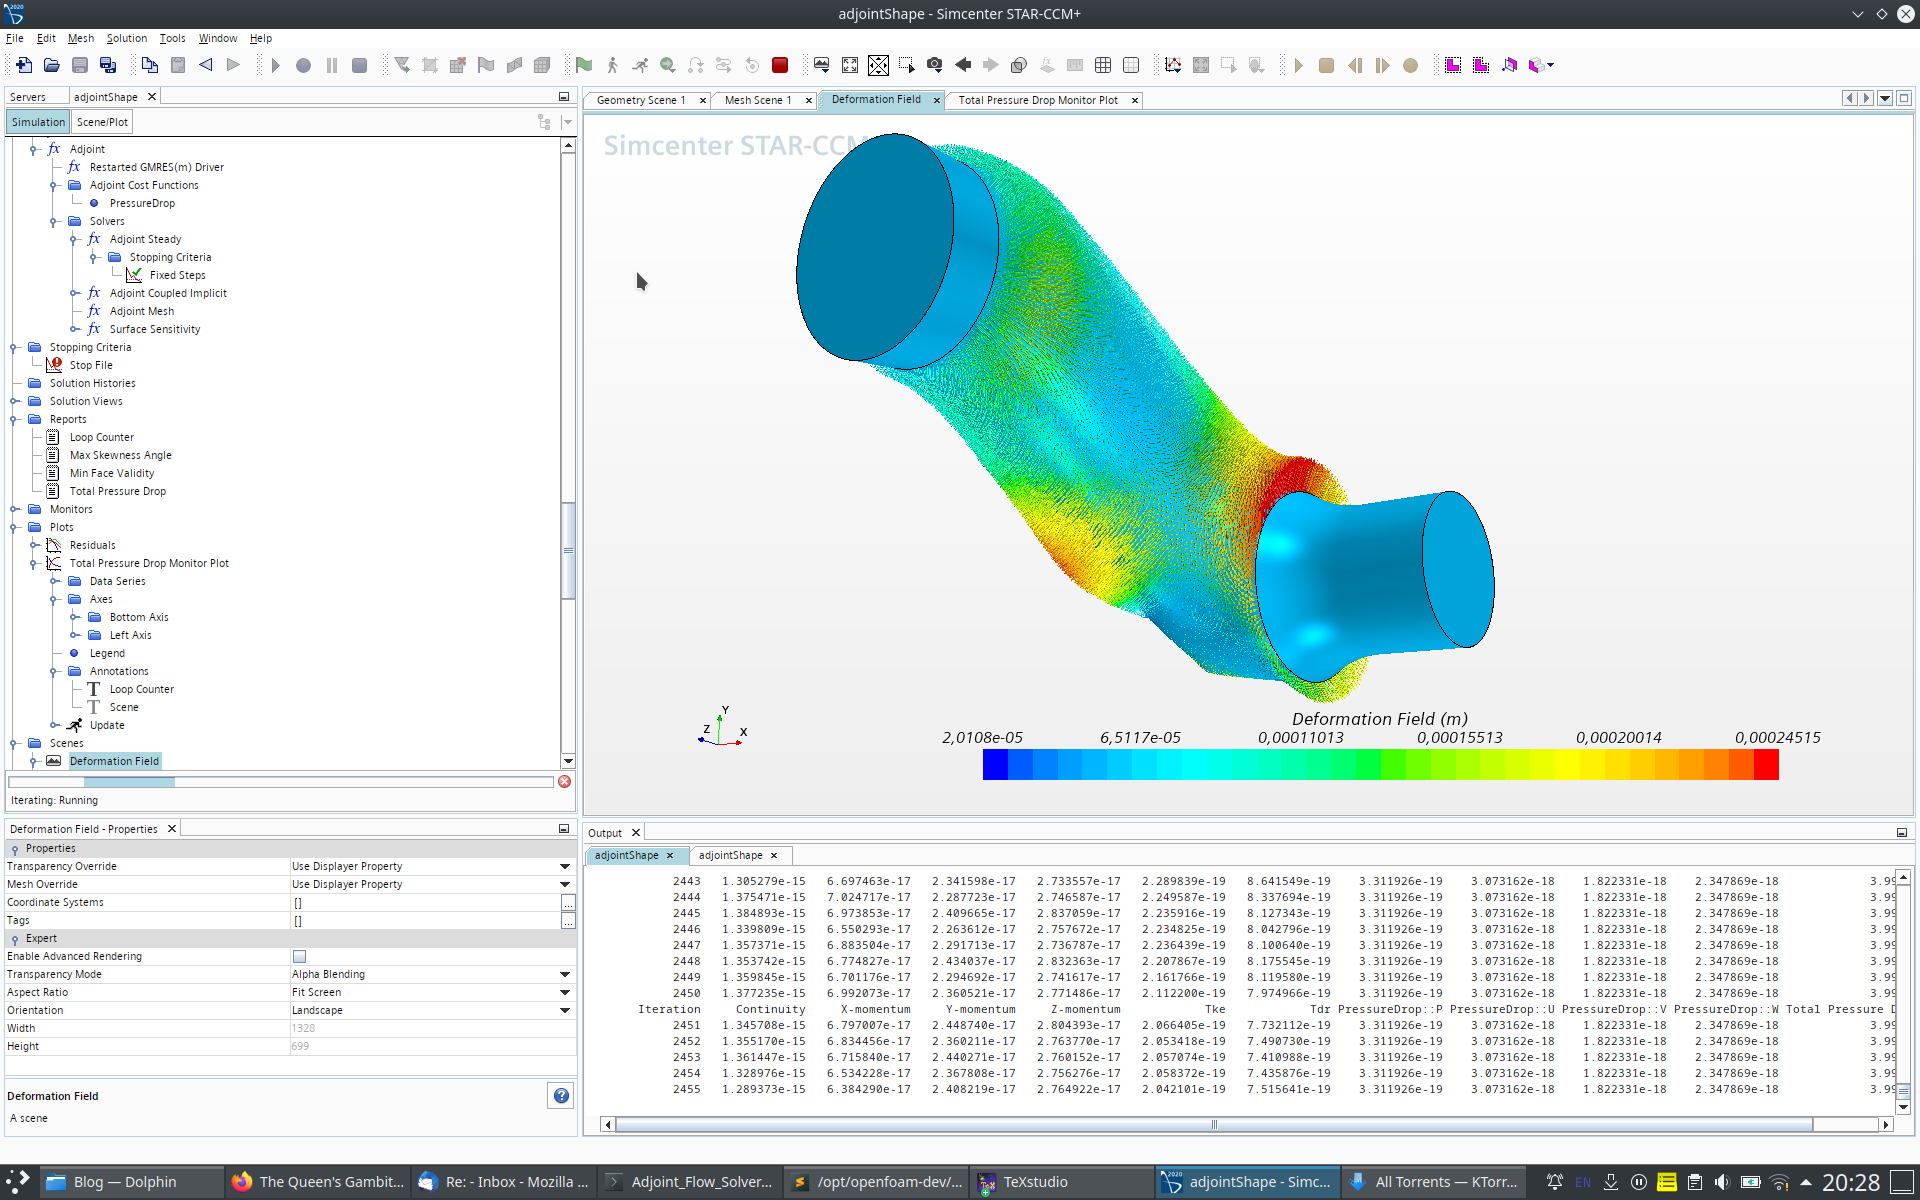
\includegraphics[height=0.44\textheight]{adjointShape_1}
            \caption{Optimized S-bend shape with the deformation field illustrated.}
        \end{figure}
        
        \begin{figure}[H]
            \centering
            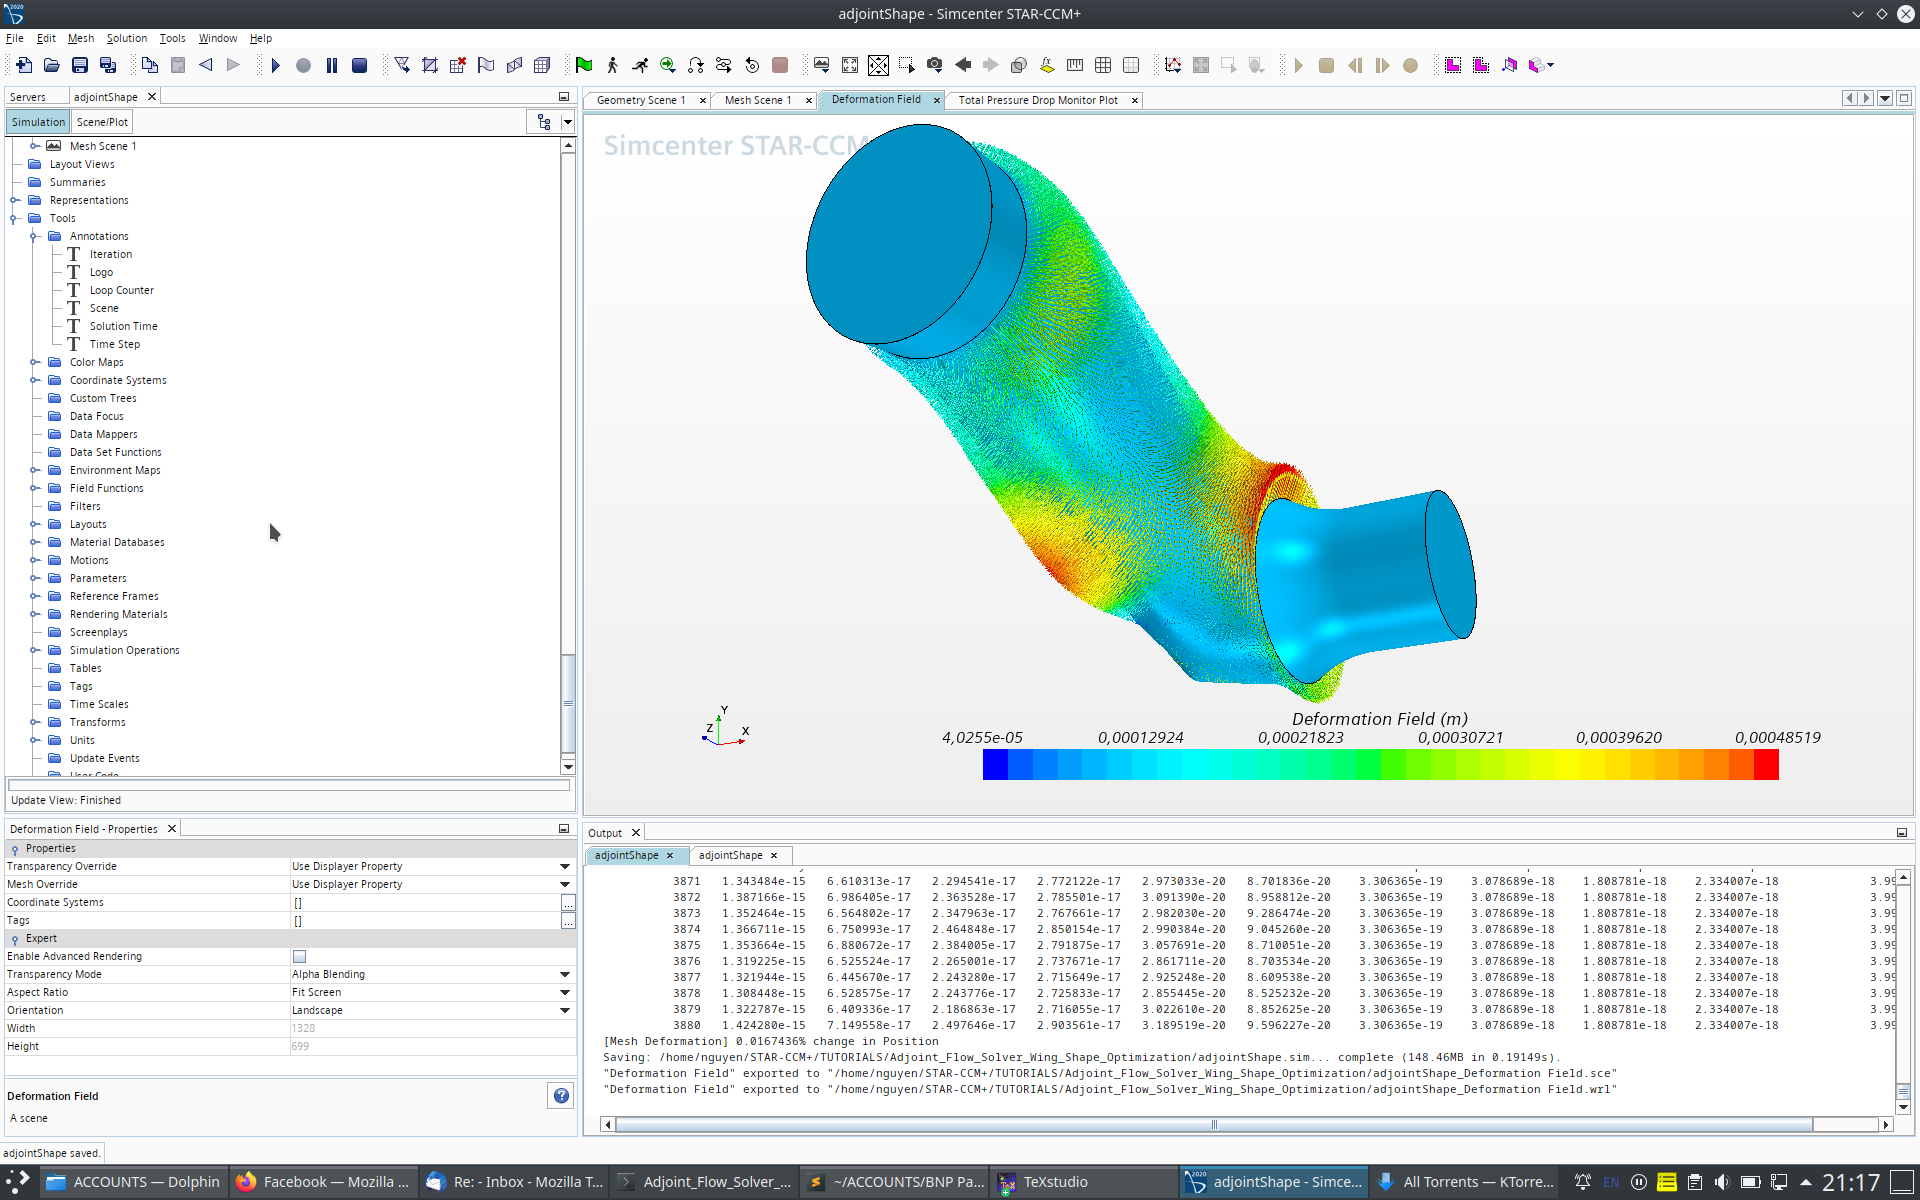
\includegraphics[height=0.44\textheight]{adjointShape_2}
            \caption{Optimized S-bend shape with the deformation field illustrated.}
        \end{figure}
    \end{enumerate}
    \item \textbf{Materials.} I have downloaded some heavy materials from the website \texttt{TheStevePortal/Support}. Besides \texttt{STAR-CCM+ Tutorial Files 15.04} and \texttt{STAR-CCM+ Verification Suite 15.04} for \textbf{Tutorials} mentioned above, these materials contains the Java macros \texttt{*.java} and predefined simulation files \texttt{*.sim} for simulation in: DIESEL, GASOLINE, NATURALGAS, NORA.
    
    $\to$ It seems to me these materials are unnecessary because of their irrelevant themes and we will eliminate \textsc{Star-CCM+} at the end anyway. Thus, I ignored all these materials.
\end{enumerate}

\section{OpenFOAM}
\begin{enumerate}
    \item \textbf{Variants.} In \href{https://en.wikipedia.org/wiki/OpenFOAM}{Wikipedia/OpenFOAM}: ``There are 3 main variants of OpenFOAM software that are released as free and open-source software under the GNU General Public License Version 3.''
    \begin{enumerate}
        \item ``OpenFOAM variant by OpenCFD Ltd. (with the name trademarked since 2007) first released as open-source in 2004. (Note that since 2012, OpenCFD Ltd is an affiliate of ESI Group.)'' $\to$ or, in short, \href{https://www.openfoam.com/}{openfoam.com}
        \item ``OpenFOAM Foundation Inc. variant, released by The OpenFOAM Foundation Inc. (since 2012), and transferred in 2015 to the English company The OpenFOAM Foundation Ltd.'' $\to$ or, in short, \href{https://openfoam.org/}{openfoam.org}
        \item ``FOAM-Extend variant by Wikki Ltd. (since 2009)'' $\to$ or, in short, \texttt{foam-extended}.
        
        \begin{remark}
            In my opinion, there is no need to pay much attention to this variant at the moment, due to the ``unofficial'' label of this variant and also the target of our project.
        \end{remark}        
    \end{enumerate}

    \begin{remark}
        I have installed and currently used the following versions of OpenFOAM:
        \begin{itemize}
            \item Notebook \texttt{nguyen@fg8nb1}:
            \begin{itemize}
                \item For \href{https://www.openfoam.com/}{openfoam.com} variant: \texttt{OpenFOAM-v2006} (release date: Jun 2020). This is not the latest version of this variant, since \href{https://www.openfoam.com/releases/openfoam-v2012/}{\texttt{OpenFOAM-v2012}} (release date: Dec 23, 2020) released recently.
                \item For \href{https://openfoam.org/}{openfoam.org} variant: \texttt{openfoam8} (latest stable version), and \texttt{openfoam-dev} (cutting-edge development, updated weekly by \texttt{sudo apt-get update} in (K)Ubuntu).
            \end{itemize}
            \item Compute server \texttt{escher-01}:
            \begin{itemize}
                \item \texttt{OpenFOAM-2.1.1} $\to$ Martin Kanitsar's \texttt{SOFTube} is only compatible with this version.
                \item \texttt{OpenFOAM-v2006}.
                
                \begin{remark}
                    Due to old version of \texttt{gcc, make}, and \texttt{cmake} on \texttt{escher-01},
                    \begin{verbatim}
nguyen@escher-01:~> gcc -v
Using built-in specs.
COLLECT_GCC=gcc
COLLECT_LTO_WRAPPER=/usr/lib64/gcc/x86_64-suse-linux/4.8/lto-wrapper
Target: x86_64-suse-linux
...
Thread model: posix
gcc version 4.8.5 (SUSE Linux)

nguyen@escher-01:~> make -v
GNU Make 4.0
Built for x86_64-unknown-linux-gnu
Copyright (C) 1988-2013 Free Software Foundation, Inc.
License GPLv3+: GNU GPL version 3 or later <http://gnu.org/licenses/gpl.html>
This is free software: you are free to change and redistribute it.
There is NO WARRANTY, to the extent permitted by law.

nguyen@escher-01:~> cmake --version
     cmake version 3.5.2
     
CMake suite maintained and supported by Kitware (kitware.com/cmake).                 
                    \end{verbatim}
                    I cannot install \texttt{openfoam-dev} on \texttt{escher-01}: it requires the newer version of \texttt{gcc, make}, and \texttt{cmake}.
                \end{remark}
            \end{itemize}
            \item Compute server \texttt{escher-03}:
            \begin{itemize}
                \item \texttt{OpenFOAM-v2006}.
                \item \texttt{openfoam-dev}.
            \end{itemize}
            \item Compute server \texttt{leonhard-01}:
            \begin{itemize}
                \item \texttt{OpenFOAM-v2006}.
                \item \texttt{openfoam-dev}.
            \end{itemize}
            Meanwhile \texttt{openfoam-dev} can be installed on other more powerful compute server, only \texttt{escher-01} has \textsc{Star-CCM+} (versions 11 and 13) installed. Thus, if I eliminate \textsc{Star-CCM+} successfully, I can run the simulation on \texttt{escher-03} or \texttt{leonhard-01} to faster runtime.
        \end{itemize}
    \end{remark}

    \begin{remark}
        Provided these versions are already compiled properly, I can switch easily between these versions of OpenFOAM by activating/uncommenting the correct line and commenting lines for other versions in the \verb|~/.bashrc| file, e.g.,
        \begin{verbatim}
. /opt/openfoam-dev/etc/bashrc
# . /opt/openfoam8/etc/bashrc
# source $HOME/OpenFOAM/OpenFOAM-2.1.1/etc/bashrc
# source $HOME/OpenFOAM/OpenFOAM-v2006/etc/bashrc
# source $HOME/OpenFOAM/OpenFOAM-dev/etc/bashrc            
        \end{verbatim}
        and source them in the current terminal
        \begin{verbatim}
source ~/.bashrc
        \end{verbatim}
        or you just need to open a new terminal and the \verb|~/.bashrc| will be sourced automatically by the nature of Unix/Linux Operating Systems.
    \end{remark}
    \item \textbf{References.}
    \begin{enumerate}
        \item For \href{https://www.openfoam.com/}{openfoam.com}:
        \begin{itemize}
            \item User Guide version v2012 (release date: Dec 22, 2020): [\href{https://sourceforge.net/projects/openfoam/files/v2012/UserGuide.pdf}{pdf}][\href{https://www.openfoam.com/documentation/user-guide}{online}].
            \item Tutorial Guide version v2012 (release date: Dec 22, 2020): [\href{https://sourceforge.net/projects/openfoam/files/v2012/TutorialGuide.pdf}{pdf}][\href{https://www.openfoam.com/documentation/tutorial-guide}{online}].
            \item Extended Code Guide v2006: [\href{https://www.openfoam.com/documentation/guides/latest/doc/}{online}].
            \item Programmer's Guide v2012: [\href{https://sourceforge.net/projects/openfoam/files/v2012/ProgrammersGuide.pdf}{pdf}].
            \item Tutorial Wiki: A community-driven collection of tutorials hosted at \url{https://wiki.openfoam.com/Main_Page}.
        \end{itemize}
        \item For \href{https://openfoam.org/}{openfoam.org}:
        \begin{itemize}
            \item User Guide version 8 (release: Jul 22, 2020) [\href{http://foam.sourceforge.net/docs/Guides-a4/OpenFOAMUserGuide-A4.pdf}{pdf}][\href{http://cfd.direct/openfoam/user-guide/}{online}]
            \item \href{https://cpp.openfoam.org/dev/}{C++ Source Code Guide for OpenFOAM-dev}: mainly used as a search tool/code-reference.
            \item \href{https://cfd.direct/openfoam/documentation/}{CFD Direct/OpenFOAM Documentation}
            \begin{itemize}
                \item \href{https://cfd.direct/openfoam/linux-guide/}{CFD Direct/OpenFOAM Linux Guide}
                \item \href{https://cfd.direct/openfoam/tensor-mathematics/}{CFD Direct/Tensor Mathematics}
                \item \href{https://cfd.direct/openfoam/energy-equation/}{CFD Direct/Energy Equation in OpenFOAM}
                
                $\to$ added to my reading list, but I have not read yet. It's quite short though.
                \item \href{https://cfd.direct/openfoam/computational-fluid-dynamics/}{CFD Direct/Computational Fluid Dynamics} 
                
                $\to$ added to my reading list, but I have not read yet. It's quite short though.
                \item \href{https://cfd.direct/openfoam/productive-cfd/}{CFD Direct/Productive CFD with OpenFOAM}
            \end{itemize}
        \end{itemize}
        \item For \texttt{foam-extended}:
        \begin{itemize}
            \item \href{https://openfoamwiki.net/index.php/Main_Page}{Unofficial OpenFOAM Wiki}.
            \item \href{http://wikki.gridcore.se/foam-extend}{\texttt{foam-extended} - the community edition}.
            \item \textbf{GitHub repository}: \href{https://github.com/Unofficial-Extend-Project-Mirrors}{Unofficial-Extend-Project-Mirror}.
        \end{itemize}
    \end{enumerate}
    
    \begin{remark}
        I have read almost all of these references, except C++ Source Code Guides, to see the big picture of OpenFOAM and which features are available. But I need time to consider these available features on theoretical side and dive deeper in C++ source codes to know how to practically make them fit to our software.
    \end{remark}
    \item \textbf{Solvers.} Based on the list of \href{https://www.openfoam.com/documentation/user-guide/standard-solvers.php}{OpenFOAM standard solvers},
    \begin{itemize}
        \item \textbf{Incompressible flow.}
        \begin{itemize}
            \item \texttt{adjointOptimisationFoam, adjointShapeOptimizationFoam}: These optimization applications are based on the series of papers of Carsten Othmer and the Greek Shape/Topology Optimization community (engineering-oriented).
            \item \texttt{icoFoam}: ``Transient solver for incompressible, laminar flow of Newtonian fluids''.
            \item \texttt{pimpleFoam}: ``Transient solver for incompressible, turbulent flow of Newtonian fluids on a moving mesh''.
            \item \texttt{pisoFoam}: ``Transient solver for incompressible, turbulent flow, using the PISO algorithm''.
            \item \texttt{simpleFoam}: ``Steady-state solver for incompressible, turbulent flows''.
        \end{itemize}
    
        \begin{remark}
            I am familiar with these incompressible solver (e.g., adjust parameters, set up initial and boundary conditions types, generate mesh by \texttt{blockMesh}) and run it separately on some simple cases. But I have not coupled, and unintended to at the moment, these solvers with Martin Kanitsar's \texttt{SOFTube/shapeGradientCCM} yet since his solver is more ``C++-oriented'' than properly ``OpenFOAM-oriented''. The folder structure is improper as forced in OpenFOAM rules. And the real trouble for me is OpenFOAM uses FVM, meanwhile a lot of components of Martin Kanitsar's \texttt{SOFTube/shapeGradientCCM} used FEM instead. There will be a big compatibility issue if I continue to develop Martin Kanitsar's \texttt{SOFTube}.
        \end{remark}
        \item \textbf{Compressible flow.} $\to$ I have not touched yet. But it seems unavoidable when I come to the part of solving adjoint equations numerically.
    \end{itemize}
    \item \textbf{Turbulence models.} A full list of available turbulence models in OpenFOAM:
    
     \url{https://cfd.direct/openfoam/user-guide/v8-turbulence/}.
     
     \begin{remark}
         At the moment, I only focus on $k$-$\epsilon$ and Smagorinsky turbulence models.
     \end{remark}
    \item \textbf{Boundary conditions.} A full list of available boundary conditions in OpenFOAM:
    
    \url{https://cfd.direct/openfoam/user-guide/v8-boundaries/}.
    
    \begin{remark}
        I need to work on theoretical side to derive their corresponding adjoint boundary conditions. And if the boundary layers and/or wall laws are involved, more investigations are needed.
    \end{remark}   
\end{enumerate}

\section{FEniCS}
\begin{enumerate}
    \item \textbf{Variants.} FEniCS, FEniCS-X (from 2021, renew almost all).
    \item \textbf{Website.} \url{https://fenicsproject.org/}.
    \item \textbf{GitHub repository.} \url{https://github.com/FEniCS}.
    \item \textbf{BitBucket repository.} \url{https://bitbucket.org/fenics-project/}.
    \item \textbf{Intro.}
    \begin{itemize}
        \item ``FEniCS is a popular open-source (\href{https://www.gnu.org/licenses/lgpl-3.0.en.html}{LGPLv3}) computing platform for solving PDEs.
        \item FEniCS enables users to quickly translate scientific models into efficient finite element code.
        \item With the high-level Python and C++ interfaces to FEniCS, it is easy to get started, but FEniCS offers also powerful capabilities for more experienced programmers.
        \item FEniCS runs on a multitude of platforms ranging from laptops to high-performance clusters.''
    \end{itemize}
    \item \textbf{Reference.} \cite{Dokken_Mitusch_Funke2020}, \cite{Langtangen_Logg2016}.
    \item \textbf{FEniCS tutorials GitHub repository.} \url{https://github.com/hplgit/fenics-tutorial}.
    \item \textbf{\href{https://fenicsproject.org/tutorial/}{Tutorials}.} I have run successfully, with some technical corrections in the Python script the following FEniCS tutorial:
    \begin{enumerate}
        \item \textbf{\href{https://github.com/hplgit/fenics-tutorial/blob/master/pub/python/vol1/ft01\_poisson.py}{Poisson's equation}.}
        
        \begin{figure}[H]
            \centering
            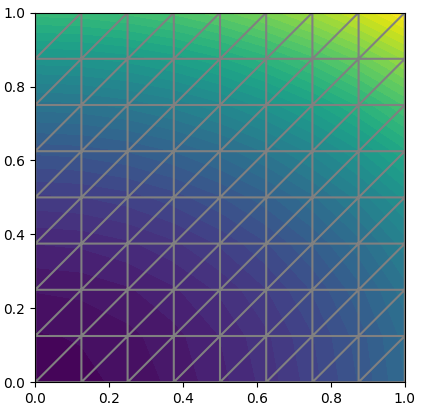
\includegraphics[width=0.5\textwidth]{ft01_poisson}
            \caption{Solution of Poisson's equation.}
        \end{figure}
        \item \textbf{\href{https://github.com/hplgit/fenics-tutorial/blob/master/pub/python/vol1/ft02\_poisson\_membrane.py}{Poisson's equation for membrane}.}
        
        \begin{figure}[H]
            \centering
            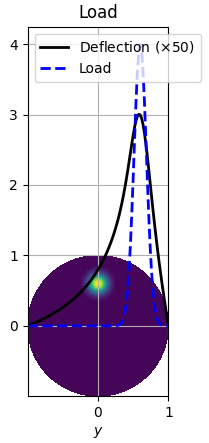
\includegraphics[width=0.3\textwidth]{ft02_poisson_membrane_curves}
            \caption{Curve for Poisson's equation for membrane.}
        \end{figure}
        \item \textbf{\href{https://github.com/hplgit/fenics-tutorial/blob/master/pub/python/vol1/ft03_heat.py}{Heat equation}.}
        
        \begin{figure}[H]
            \centering
            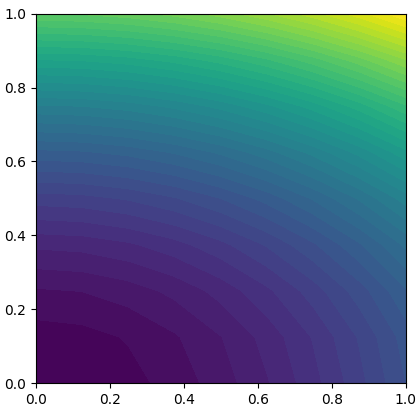
\includegraphics[width=0.5\textwidth]{ft03_heat}
            \caption{Solution of heat equation.}
        \end{figure}
        \item \textbf{\href{https://github.com/hplgit/fenics-tutorial/blob/master/pub/python/vol1/ft04_heat_gaussian.py}{Heat equation with Gaussian}.}
        
        \begin{figure}[H]
            \centering
            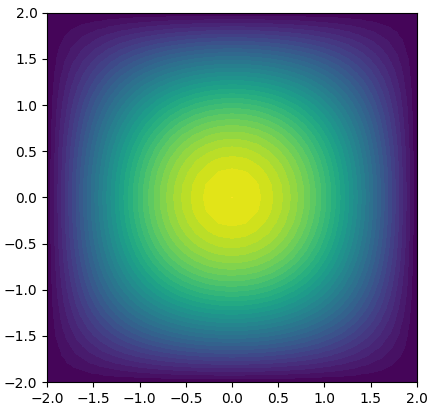
\includegraphics[width=0.5\textwidth]{ft04_heat_gaussian}
            \caption{Solution of heat equation with Gaussian.}
        \end{figure}
        \item \textbf{\href{https://github.com/hplgit/fenics-tutorial/blob/master/pub/python/vol1/ft05_poisson_nonlinear.py}{Nonlinear Poisson's equation}.}
        
        \begin{figure}[H]
            \centering
            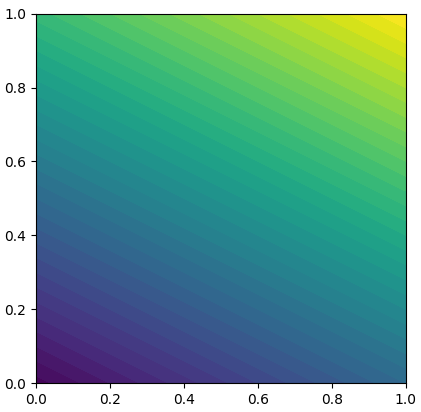
\includegraphics[width=0.5\textwidth]{ft05_poisson_nonlinear}
            \caption{Solution of nonlinear Poisson's equation.}
        \end{figure}
        \item \textbf{\href{https://github.com/hplgit/fenics-tutorial/blob/master/pub/python/vol1/ft06_elasticity.py}{Elasticity}.}
        
        \begin{figure}[H]
            \centering
            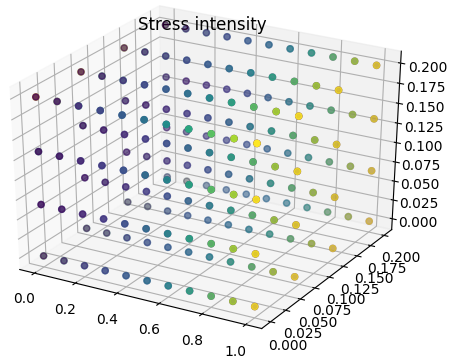
\includegraphics[width=0.5\textwidth]{ft06_elasticity}
            \caption{Elasticity.}
        \end{figure}
        \item \textbf{\href{https://github.com/hplgit/fenics-tutorial/blob/master/pub/python/vol1/ft07_navier_stokes_channel.py}{Navier-Stokes flow in a channel}.}
        
        \begin{figure}[H]
            \centering
            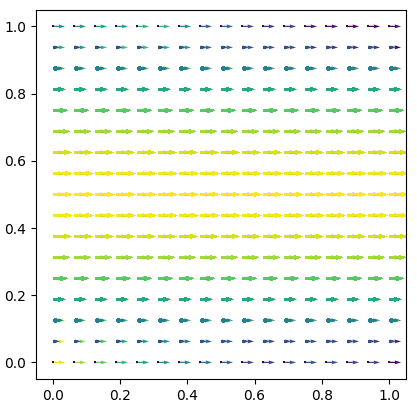
\includegraphics[width=0.5\textwidth]{ft07_navier_stokes_channel}
            \caption{Velocity of Navier-Stokes flows in a channel.}
        \end{figure}
        \item \textbf{\href{https://github.com/hplgit/fenics-tutorial/blob/master/pub/python/vol1/ft08_navier_stokes_cylinder.py}{Navier-Stokes flows in a cylinder}.}
        
        \begin{figure}[H]
            \centering
            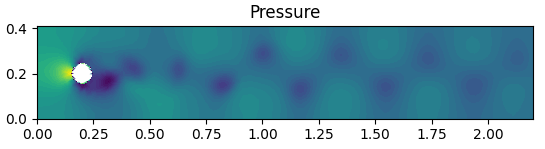
\includegraphics[width=0.7\textwidth]{ft08_navier_stokes_cylinder_pressure}
            \caption{Pressure $p$ of Navier-Stokes flows in a cylinder.}
        \end{figure}
    
        \begin{figure}[H]
            \centering
            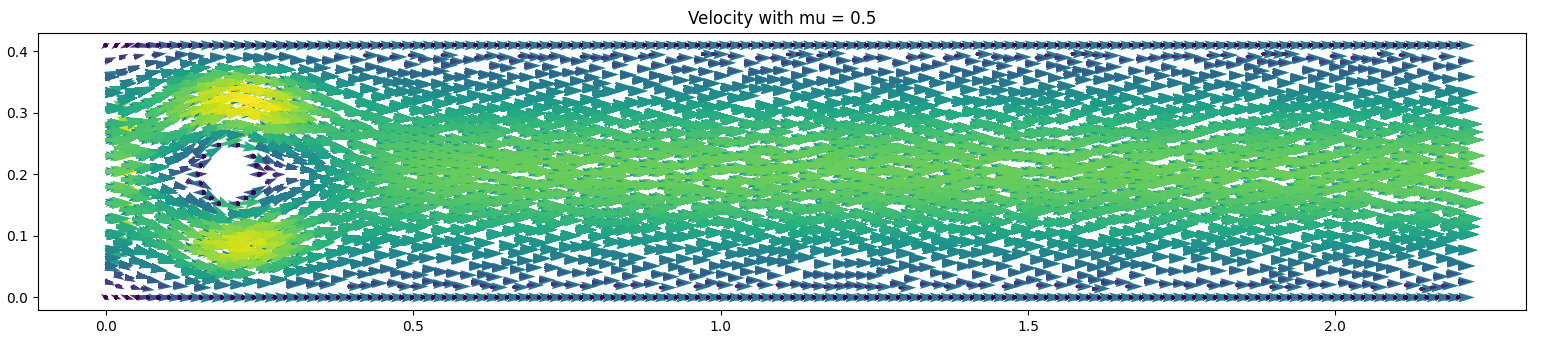
\includegraphics[width=0.7\textwidth]{ft08_navier_stokes_cylinder_velocity_viscosity_05}
            \caption{Velocity ${\bf u}$ of Navier-Stokes flows in a cylinder with viscosity $\mu = 0.5$.}
        \end{figure}
    
        \begin{figure}[H]
            \centering
            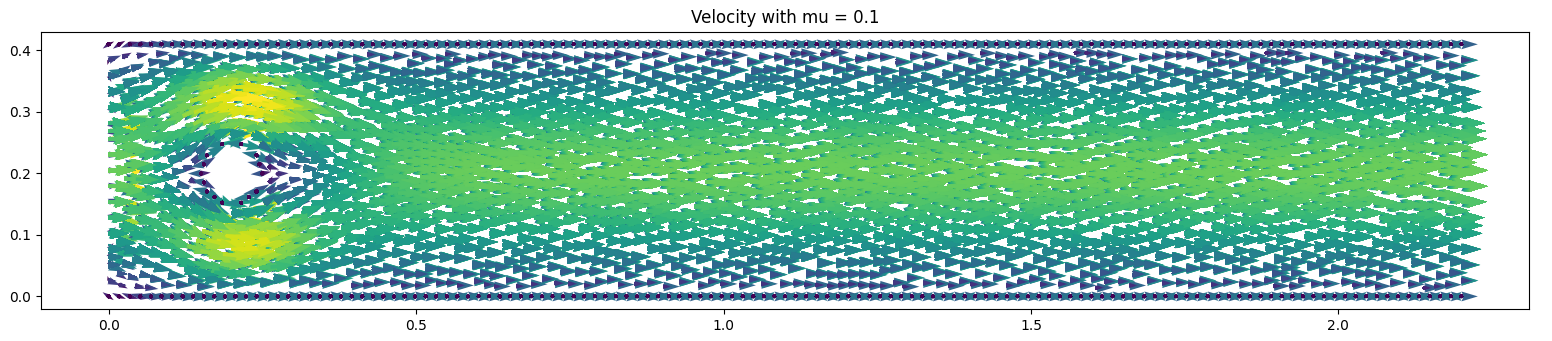
\includegraphics[width=0.7\textwidth]{ft08_navier_stokes_cylinder_velocity_viscosity_01}
            \caption{Velocity ${\bf u}$ of Navier-Stokes flows in a cylinder with viscosity $\mu = 0.1$.}
        \end{figure}
    
        \begin{figure}[H]
            \centering
            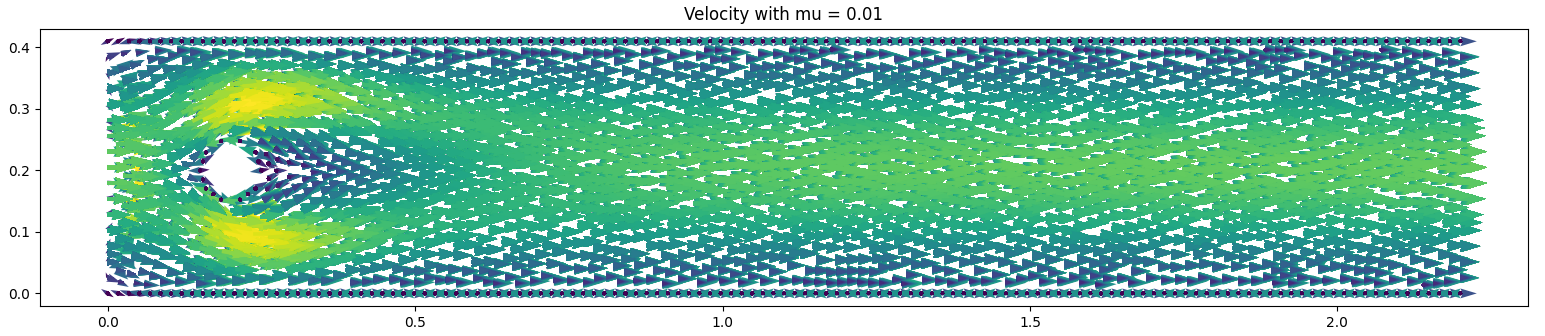
\includegraphics[width=0.7\textwidth]{ft08_navier_stokes_cylinder_velocity_viscosity_001}
            \caption{Velocity ${\bf u}$ of Navier-Stokes flows in a cylinder with viscosity $\mu = 0.01$.}
        \end{figure}
    
        \begin{figure}[H]
            \centering
            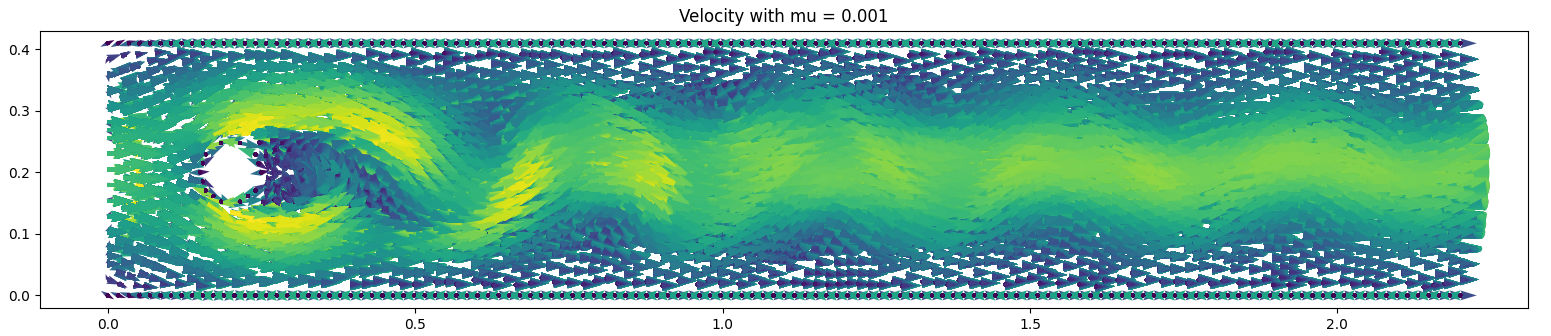
\includegraphics[width=0.7\textwidth]{ft08_navier_stokes_cylinder_velocity_viscosity_0001}
            \caption{Velocity ${\bf u}$ of Navier-Stokes flows in a cylinder with viscosity $\mu = 0.001$.}
        \end{figure}
    \end{enumerate}
    \item \textbf{Materials.} Stephan Schmidt's course + codes on \textit{Shape and Geometry}.
\end{enumerate}

\section{Firedrake}
\begin{enumerate}
    \item \textbf{Website.} \url{https://www.firedrakeproject.org/}
    \item \textbf{GitHub repository.} \url{https://github.com/firedrakeproject/firedrake}
    \item \textbf{Intro.} ``\textit{Firedrake is an automated system for the solution of PDEs using the FEM. Firedrake uses sophisticated code generation to provide mathematicians, scientists, and engineers with a very high productivity way to create sophisticated high performance simulations.}''
    \item \textbf{Features.}
    \begin{itemize}
        \item ``Expressive specification of any PDE using the Unified Form Language from \href{http://fenicsproject.org/}{the FEniCS Project}.
        \item Sophisticated, programmable solvers through seamless coupling with PETSc.
        \item Triangular, quadrilateral, and tetrahedral unstructured meshes.
        \item Layered meshes of triangular wedges or hexahedra.
        \item Vast range of finite element spaces.
        \item Sophisticated automatic optimization, including sum factorization for high order elements, and vectorization.
        \item Geometric multigrid.
        \item Customizable operator preconditioners.
        \item Support for static condensation, hybridization, and HDG methods.''
    \end{itemize}
    \item \textbf{Reference.} [inserted original article(s)]
    \item \textbf{Documentation.} \url{https://www.firedrakeproject.org/documentation.html}
    \item \textbf{Introductory tutorials.} I have run successfully:
    \begin{itemize}
        \item \href{https://www.firedrakeproject.org/demos/helmholtz.py.html}{\textbf{Simple Helmholtz equation}}:
        \begin{equation*}
            \left\{\begin{split}
                -\Delta u + u &= f &&\mbox{ in } \Omega = [0,1]^2,\\
                \partial_{\bf n}u &= 0 &&\mbox{ on } \Gamma.
            \end{split}\right.
        \end{equation*}
        \item \href{https://www.firedrakeproject.org/demos/burgers.py.html}{\textbf{Burgers equation}}: $\nu > 0$ is a constant viscosity,
        \begin{equation*}
            \left\{\begin{split}
                \partial_t{\bf u} + ({\bf u}\cdot\nabla){\bf u} - \nu\Delta{\bf u} &= {\bf 0} &&\mbox{ in } \Omega = [0,1]^2,\\
                ({\bf n}\cdot\nabla){\bf u} &= 0 &&\mbox{ on } \Gamma.
            \end{split}\right.
        \end{equation*}
        \item \href{https://www.firedrakeproject.org/demos/poisson_mixed.py.html}{\textbf{Mixed formulation for the Poisson equation}}: Introduce the negative flux $\boldsymbol{\sigma} = \nabla u$ as an auxiliary vector-valued variable,
        \begin{equation*}
            \left\{\begin{split}
                \boldsymbol{\sigma} - \nabla u &= 0 &&\mbox{ on } \Omega = [0,1]^2,\\
                \nabla\cdot\boldsymbol{\sigma} &= -f &&\mbox{ on } \Omega,\\
                u &= u_0 &&\mbox{ on } \Gamma_{\rm D},\\
                \boldsymbol{\sigma}\cdot{\bf n} &= g &&\mbox{ on } \Gamma_{\rm N}.
            \end{split}\right.
        \end{equation*}
        \item \href{https://www.firedrakeproject.org/demos/DG_advection.py.html}{\textbf{DG advection equation with upwinding}}: Advection equation
        \begin{equation*}
            \left\{\begin{split}
                \partial_tq + ({\bf u}\cdot\nabla)q &= 0 &&\mbox{ in } [0,T]\times\Omega,\\
                q(0,{\bf x}) &= q_0({\bf x}) &&\mbox{ in } \Omega,\\
                q(t,{\bf x}) &= q_{\rm in}(t,{\bf x}) &&\mbox{ on } \Gamma_{\rm inflow}.
            \end{split}\right.
        \end{equation*}
        \item \href{https://www.firedrakeproject.org/demos/extruded_continuity.py.html}{\textbf{Steady-state continuity equation on an extruded mesh}}: Use of extruded meshes, including the new regions of integration and the construction of sophisticated FE spaces.
        \begin{equation*}
            \left\{\begin{split}
                \nabla\cdot(q{\bf u}) &= 0 &&\mbox{ in } \Omega,\\
                q &= q_{\rm in} &&\mbox{ on } \Gamma_{\rm inflow}.
            \end{split}\right.
        \end{equation*}
        \item \href{https://www.firedrakeproject.org/demos/linear_wave_equation.py.html}{\textbf{Double slit experiment}}: Solve a linear wave equation using an explicit timestepping scheme. Demonstrate the use of an externally generated mesh, pointwise operations on Functions, and a time varying boundary condition:
        \begin{equation*}
            \left\{\begin{split}
                \partial_t^2\phi - \Delta\phi &= 0 &&\mbox{ in } [0,T]\times\Omega,\\
                \partial_{\bf n}\phi &= 0 &&\mbox{ on } \Gamma_{\rm N},\\
                \phi &= \frac{1}{10\pi}\cos\left(10\pi t\right) &&\mbox{ on } \Gamma_{\rm D}.
            \end{split}\right.
        \end{equation*}
        Make the substitution to facilitate the choice of time integrator:
        \begin{equation*}
            \left\{\begin{split}
                \partial_t\phi &= -p &&\mbox{ in } [0,T]\times\Omega,\\
                \partial_tp + \Delta\phi &= 0 &&\mbox{ in } [0,T]\times\Omega,\\
                \partial_{\bf n}\phi &= 0 &&\mbox{ on } \Gamma_{\rm N},\\
                p &= \sin\left(10\pi t\right) &&\mbox{ on } \Gamma_{\rm D},
            \end{split}\right.
        \end{equation*}
        \item \href{https://www.firedrakeproject.org/demos/immersed_fem.py.html}{\textbf{Creating Firedrake-compatible meshes in Gmsh}}: Key structure of a \texttt{gmsh.geo} file that creates a Firedrake-compatible mesh.
    \end{itemize}
\end{enumerate}

\section{Fireshape}
\begin{enumerate}
    \item \textbf{Website.} \url{https://fireshape.readthedocs.io/en/latest/}
    \item \textbf{GitHub repository.} \url{https://github.com/fireshape/fireshape}
    \item \textbf{Overview.} ``Fireshape is a shape optimization toolbox for the finite element library \href{https://www.firedrakeproject.org/}{Firedrake}.''
    
    \textbf{Inputs.} ``To set up a shape optimization problem, all you need to provide is the mesh on an initial guess, the shape functional, and the weak-form of its PDE-contraint.''
    
    ``Fireshape computes adjoints and assembles first and second derivatives for you using \href{http://www.dolfin-adjoint.org/en/release/}{pyadjoint}, and it solves the optimization problem using the rapid optimization library (\href{https://trilinos.org/packages/rol/}{ROL}).''
    \item \textbf{Features.}
    \begin{itemize}
        \item ``Fireshape neatly distinguishes between the discretization of control and state variables.
        \begin{itemize}
            \item To discretize the control, you can choose among finite elements, B-splines, and the free-form approach.
            \item To discretize the state, you have access to all finite element spaces offered by Firedrake.
        \end{itemize}
        \item Fireshape relies on the mesh-deformation approach to update the geometry of the domain.
        
        By specifying the metric of the control space, you can decide whether meshes should be updated using Laplace or elasticity equations.
        
        In 2D, you can also use the elasticity equation corrected with Cauchy-Riemann terms, which generally leads to very high-quality meshes.''
    \end{itemize}
    \item \textbf{Documentation.} \cite{Paganini_Wechsung_Fireshape2020}.
    \item \textbf{Reference.} \cite{Paganini_Wechsung2020}.
    \item \textbf{Installation.} I have installed Fireshape version 1.0 successfully in VirtualBox Ubuntu 18.04.4. I need to do this, because:
    \begin{itemize}
        \item The version of Python Fireshape requires matches exactly the default version of Python Ubuntu 18.04.4 have.
        \item After having installed Fireshape on Ubuntu, FEniCS does not work properly anymore. Because of this conflict, which seems to involve Python versions again, I use VirtualBox Ubuntu instead. But working with a virtual machine slows down considerably the whole simulation process because of, e.g.:
        \begin{itemize}
            \item switch to VirtualBox,
            \item running time of Fireshape with partially (less than half) distributed memory, then switch back to the host machine,
            \item shared folder trouble between host and virtual machines.
        \end{itemize}
    \end{itemize}
    
    \begin{remark}
        Because I will focus more on FEniCS than Fireshape, I have not tested the compatibility of Fireshape version 2.0 to Ubuntu 20.04 to protect FEniCS installed in my notebook.
    \end{remark}
    \item \textbf{Tutorials.} I have run successfully:
    \begin{enumerate}
        \item \href{https://fireshape.readthedocs.io/en/latest/example_levelset.html#example-levelset}{\textbf{Example 1: Level Set}}: Minimize the shape functional
        \begin{align*}
            J(\Omega) := \int_\Omega f({\bf x}){\rm d}{\bf x}, \mbox{ where } f(x,y) = \left(x - \frac{1}{2}\right)^2 + \left(y - \frac{1}{2}\right)^2 - \frac{1}{2}.
        \end{align*}
        Optimal solution:
        \begin{align*}
            \Omega_{\rm opt} := B_{1/\sqrt{2}}\left(\left(\frac{1}{2},\frac{1}{2}\right)\right).
        \end{align*}
        \textbf{Numerical results.}
        
        \begin{figure}[H]
            \centering
            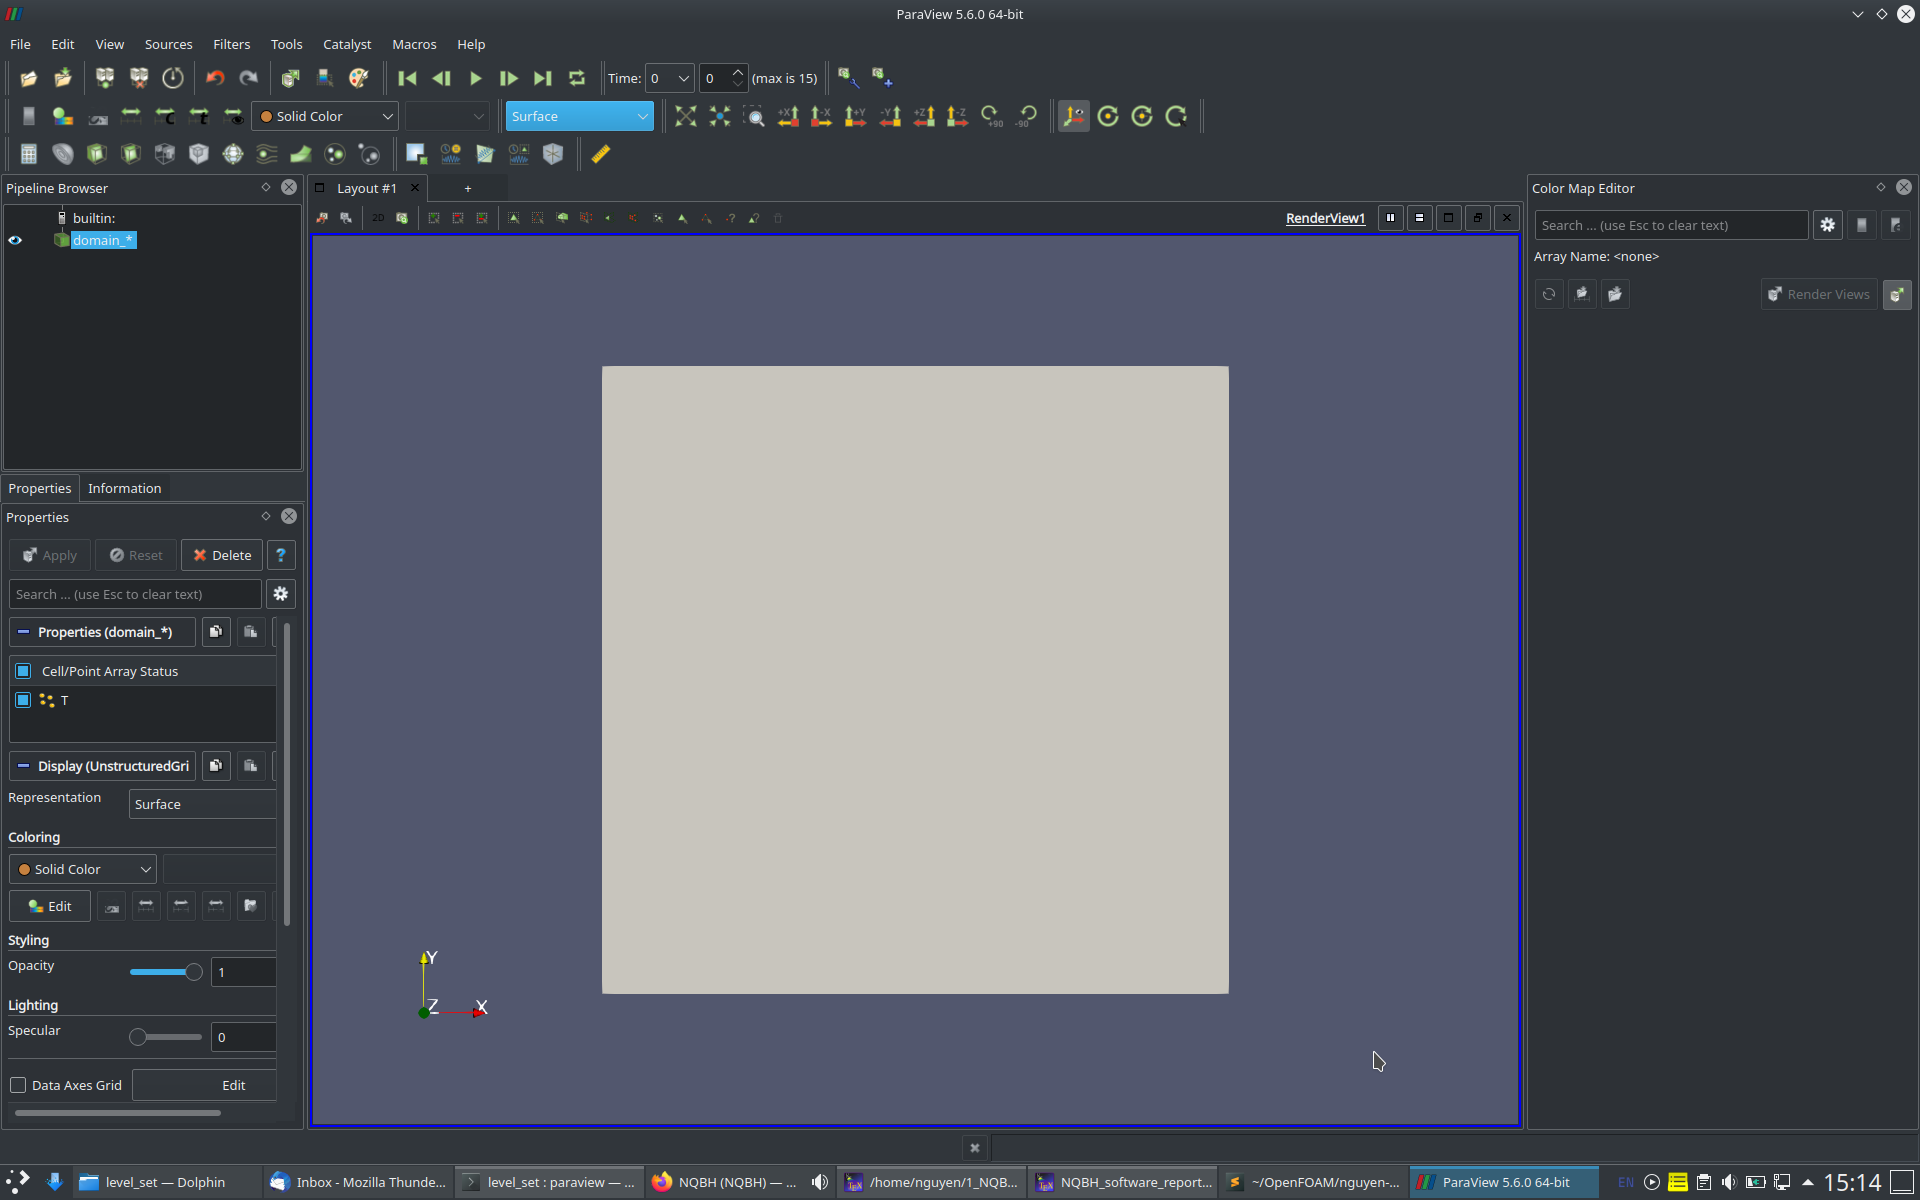
\includegraphics[height=0.44\textheight]{level_set_initial_domain_Solid_Color_Surface}
            \caption{View the initial domain by ParaView with modes: \texttt{Solid Color, Surface}.}
        \end{figure}
    
        \begin{figure}[H]
            \centering
            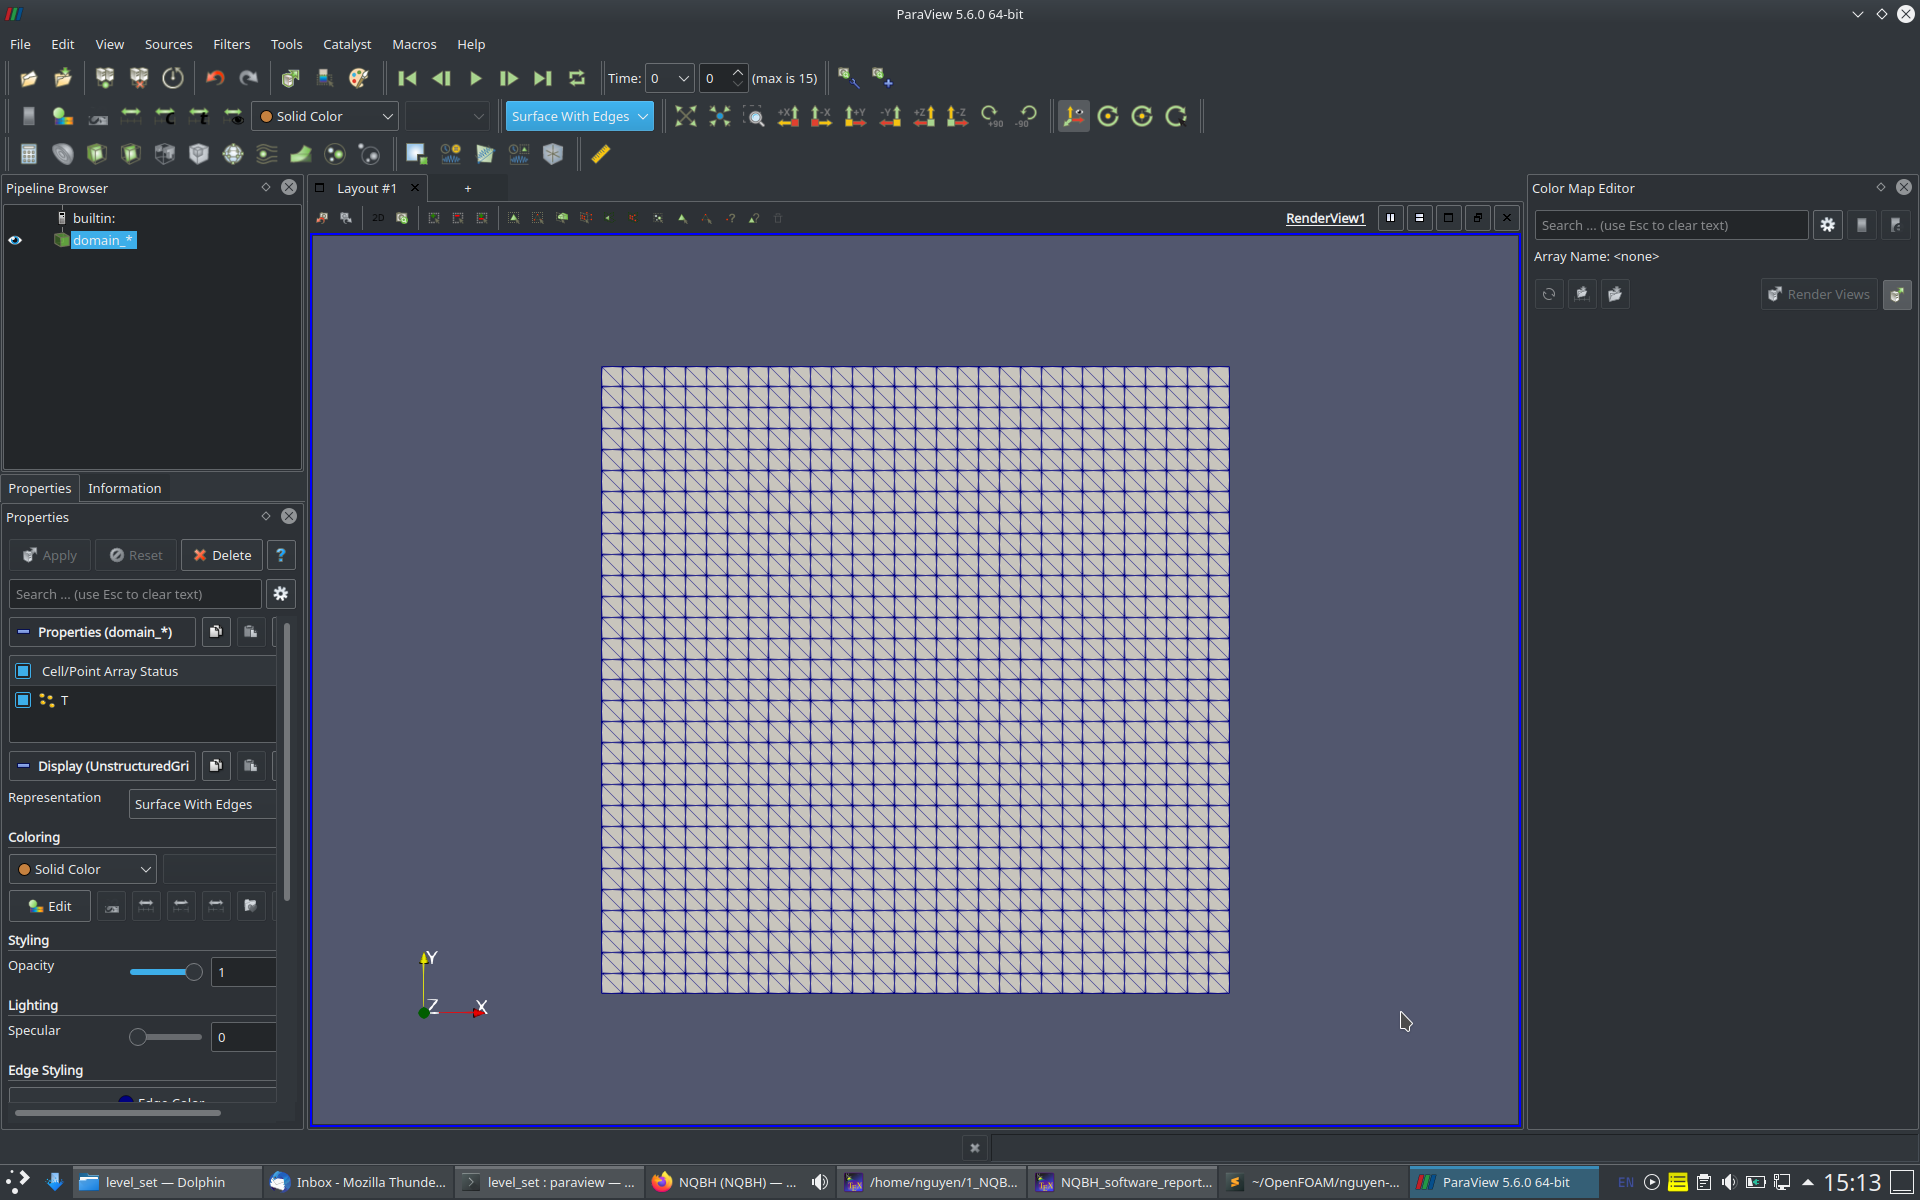
\includegraphics[height=0.44\textheight]{level_set_initial_domain_Solid_Color_Surface_with_Edges}
            \caption{View the initial domain by ParaView with modes: \texttt{Solid Color, Surface with Edges}.}
        \end{figure}
    
        %
        \begin{figure}[H]
            \centering
            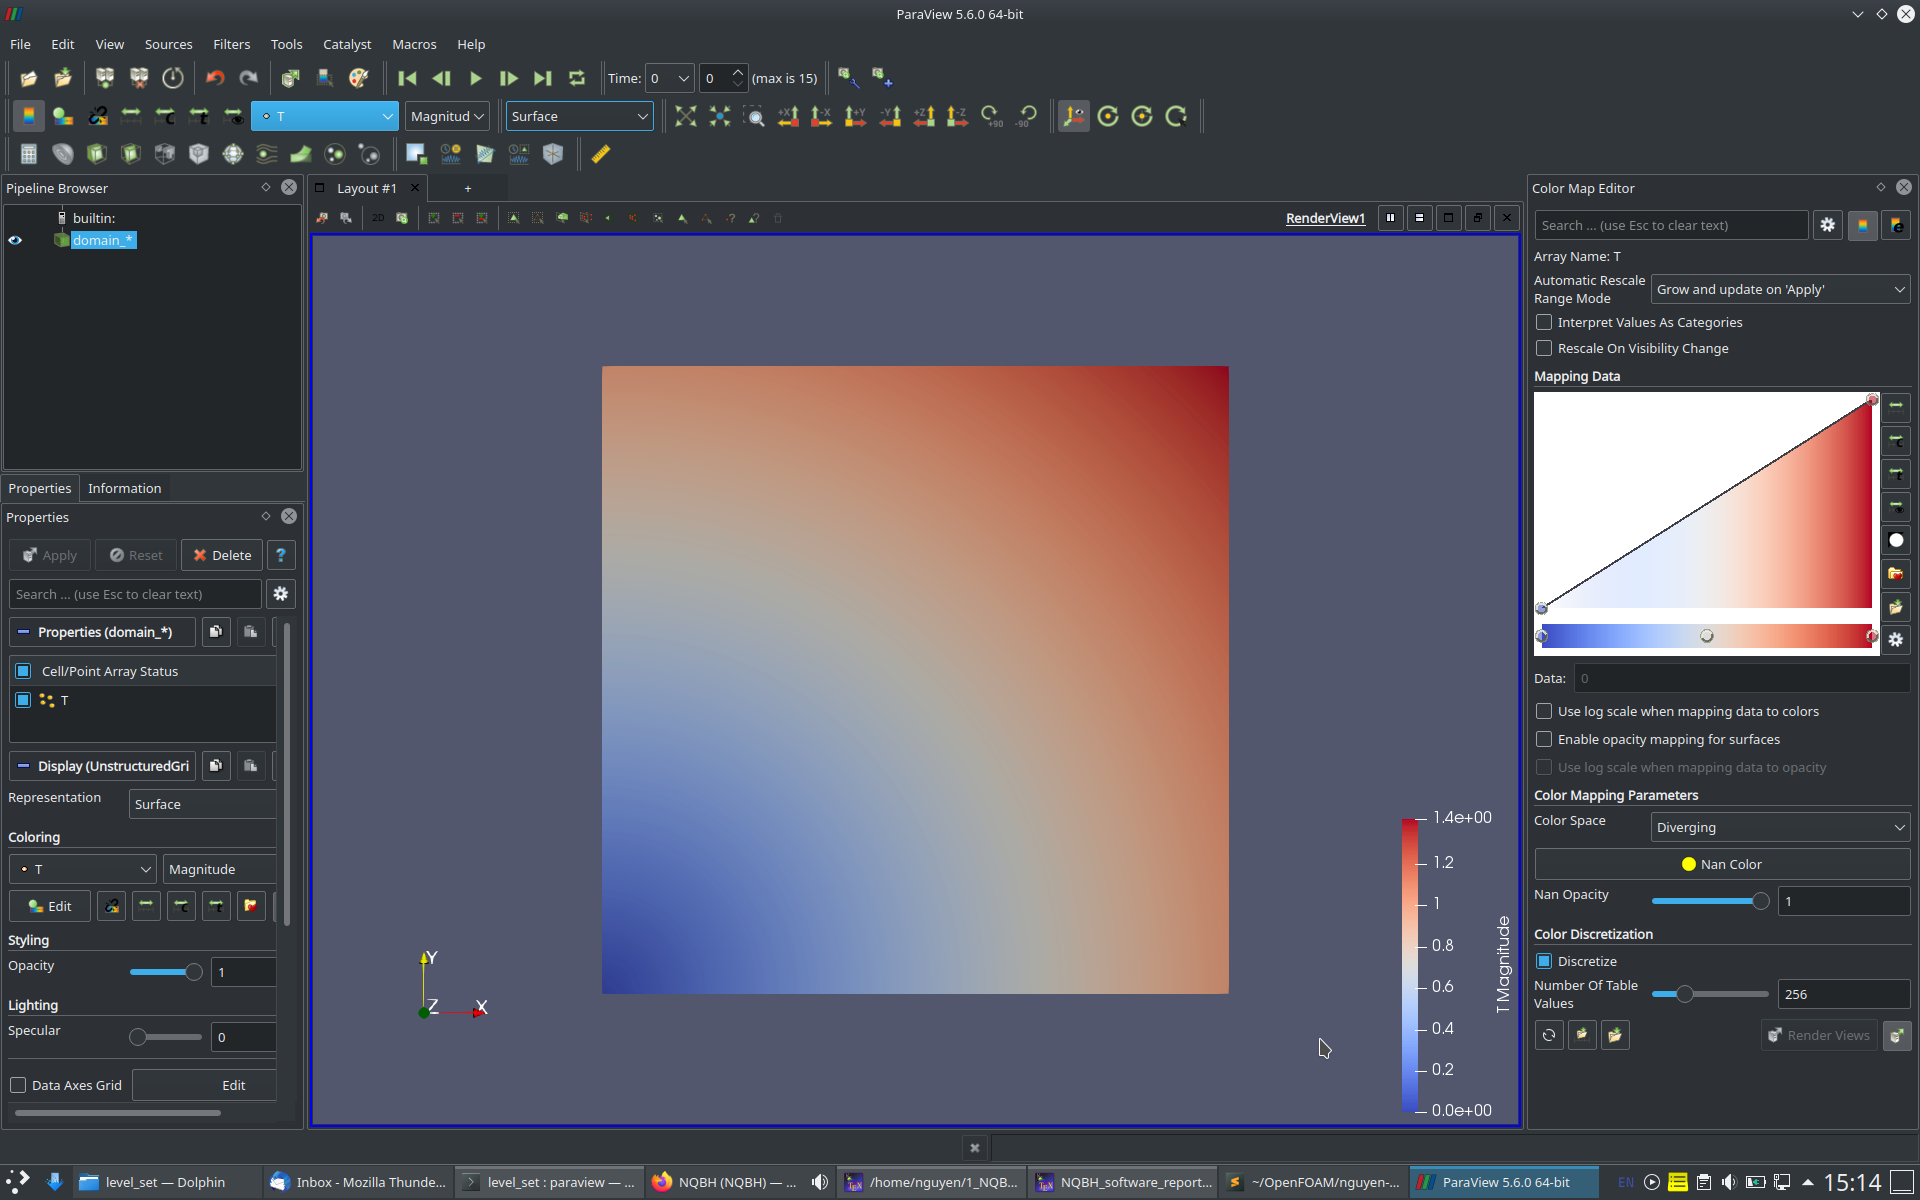
\includegraphics[height=0.44\textheight]{level_set_initial_domain_T_Surface}
            \caption{View the initial domain by ParaView with modes: \texttt{$T$, Surface}.}
        \end{figure}
        
        \begin{figure}[H]
            \centering
            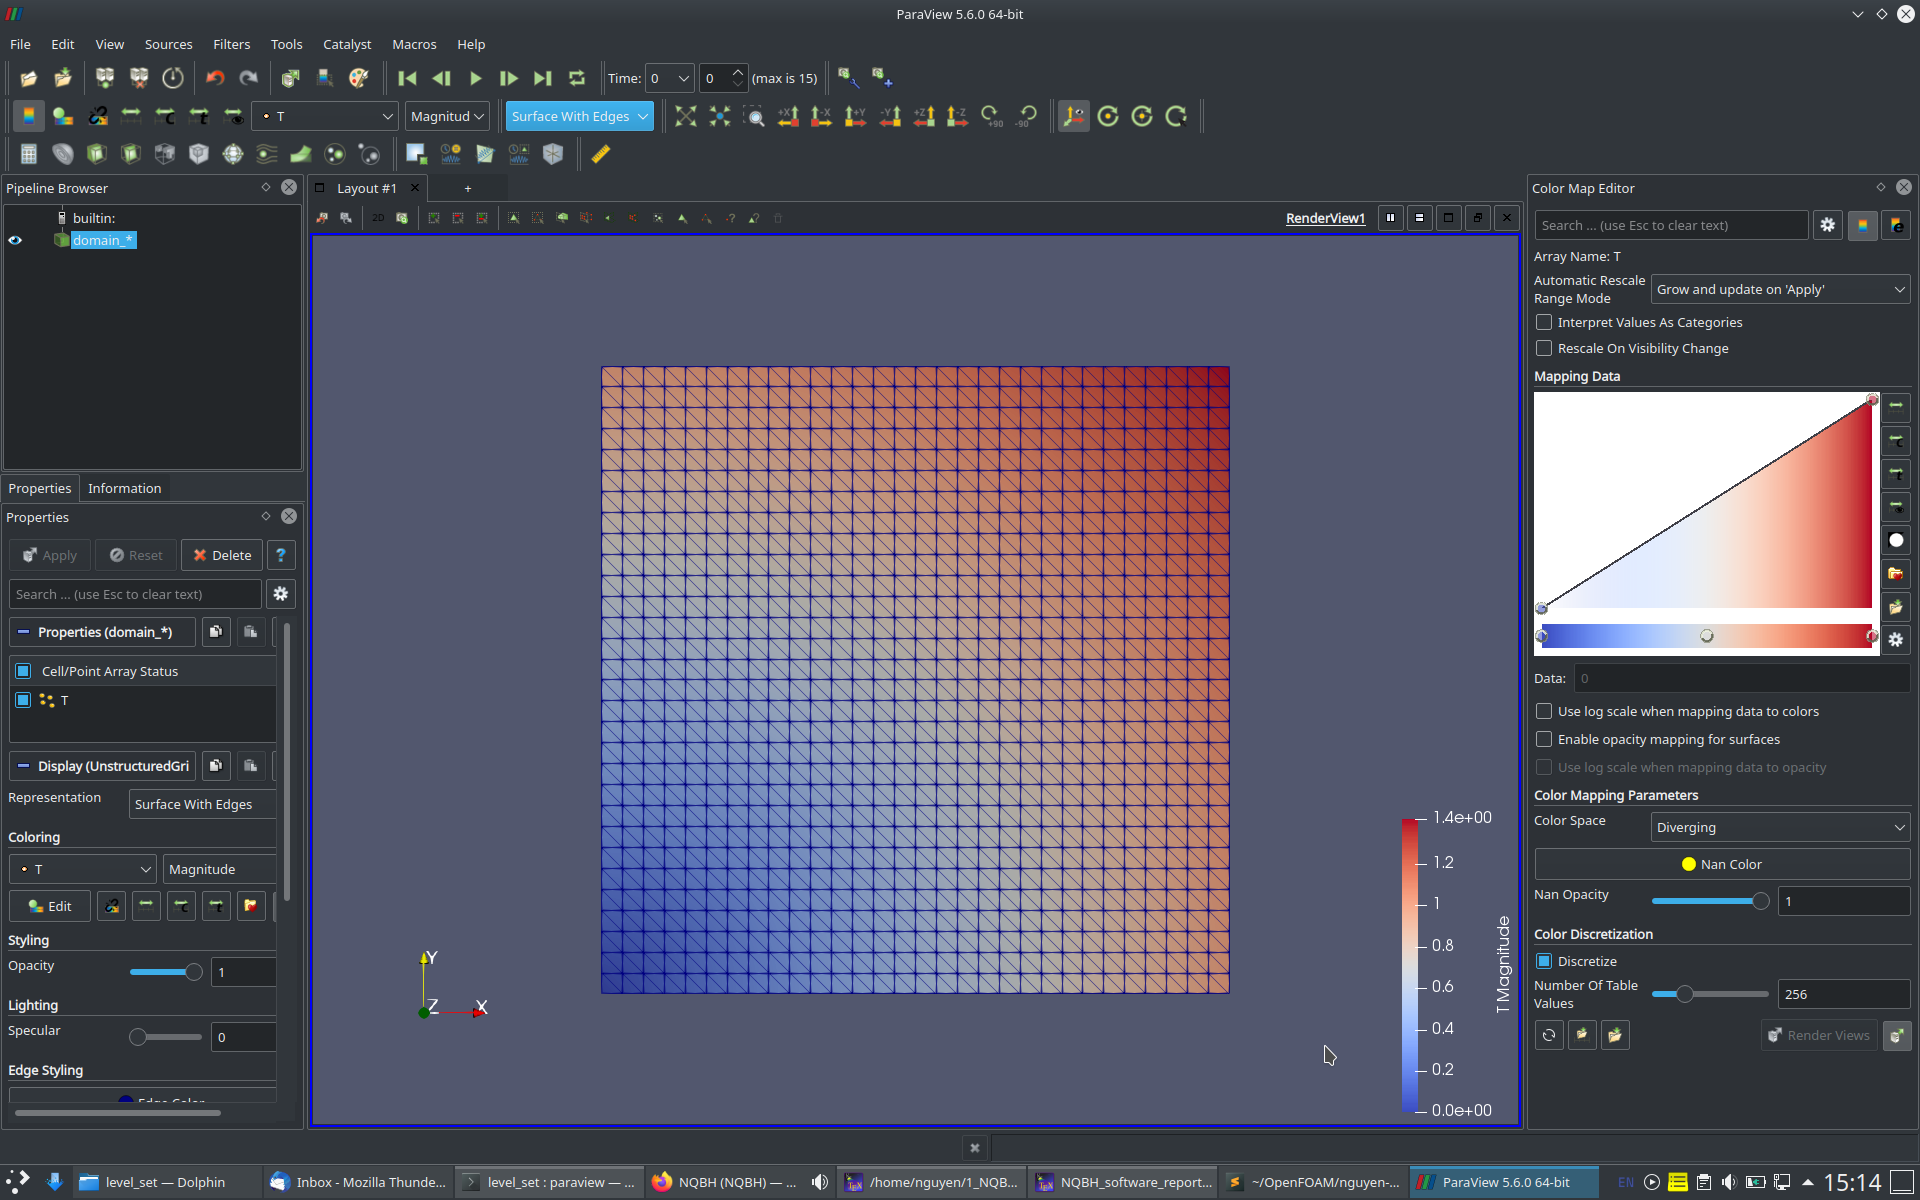
\includegraphics[height=0.44\textheight]{level_set_initial_domain_T_Surface_with_Edges}
            \caption{View the initial domain by ParaView with modes: \texttt{$T$, Surface with Edges}.}
        \end{figure}
        
        %
        \begin{figure}[H]
            \centering
            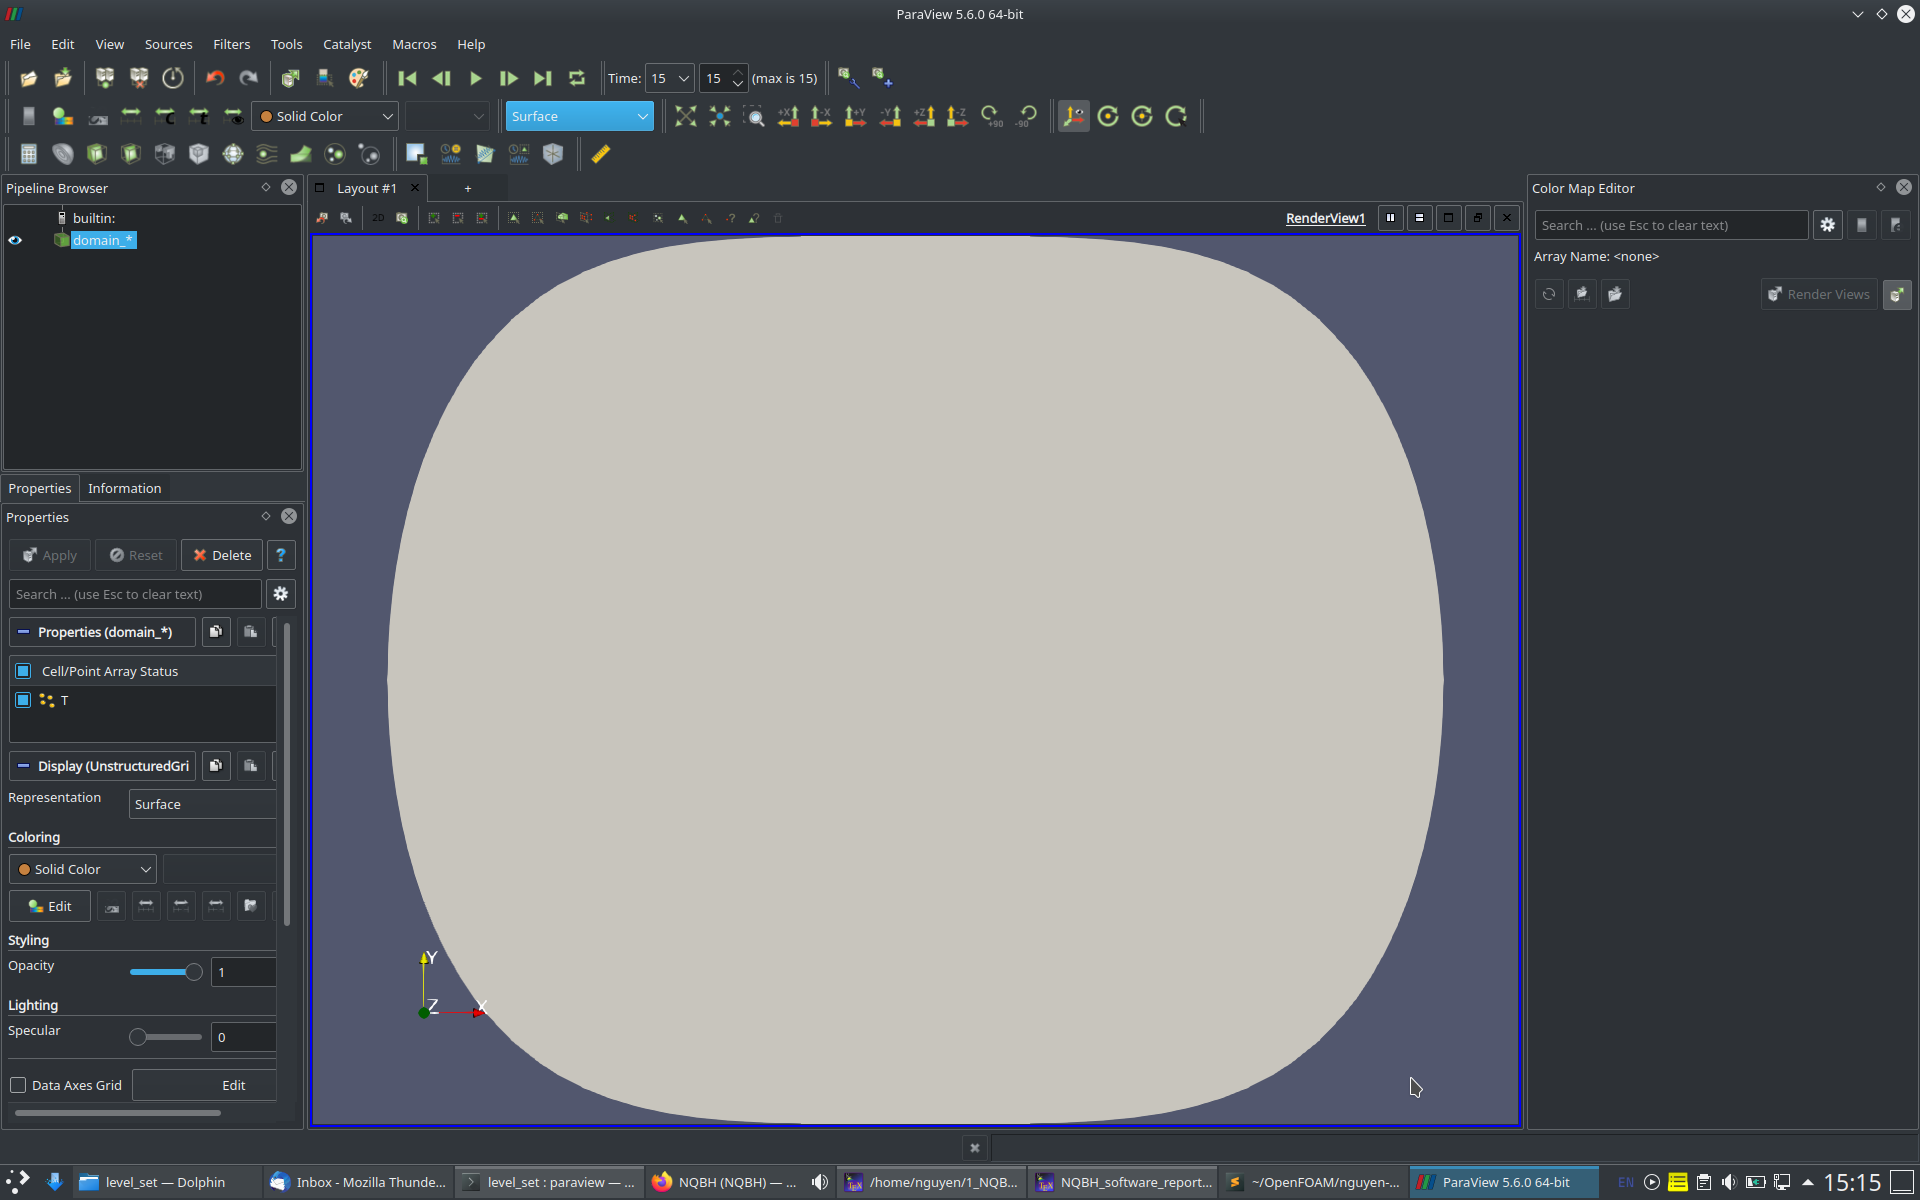
\includegraphics[height=0.44\textheight]{level_set_optimized_domain_after_15_steps_Solid_Color_Surface}
            \caption{View the optimized domain after 15 optimization steps by ParaView with modes: \texttt{Solid Color, Surface}.}
        \end{figure}
        
        \begin{figure}[H]
            \centering
            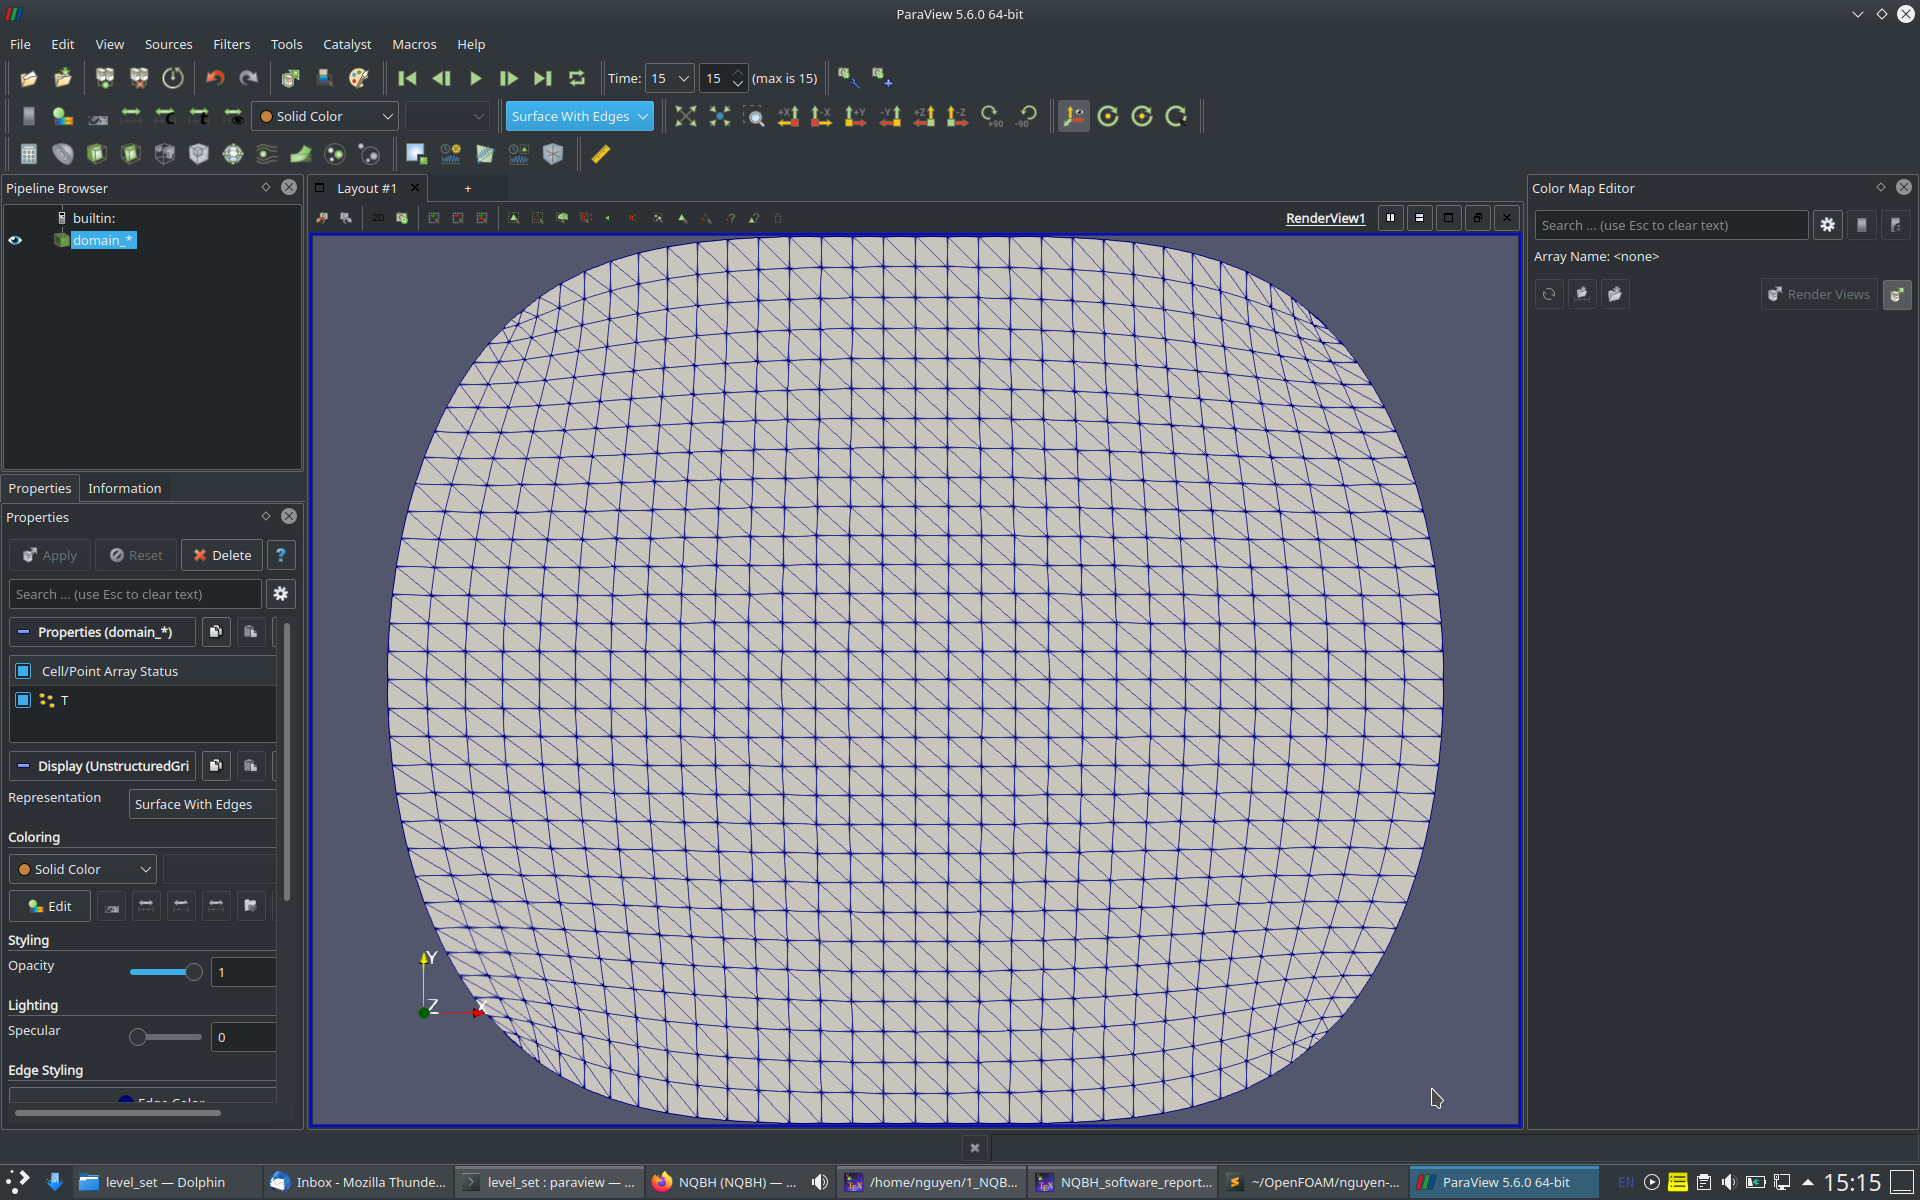
\includegraphics[height=0.44\textheight]{level_set_optimized_domain_after_15_steps_Solid_Color_Surface_with_Edges}
            \caption{View the optimized domain after 15 optimization steps by ParaView with modes: \texttt{Solid Color, Surface with Edges}.}
        \end{figure}
        
        %
        \begin{figure}[H]
            \centering
            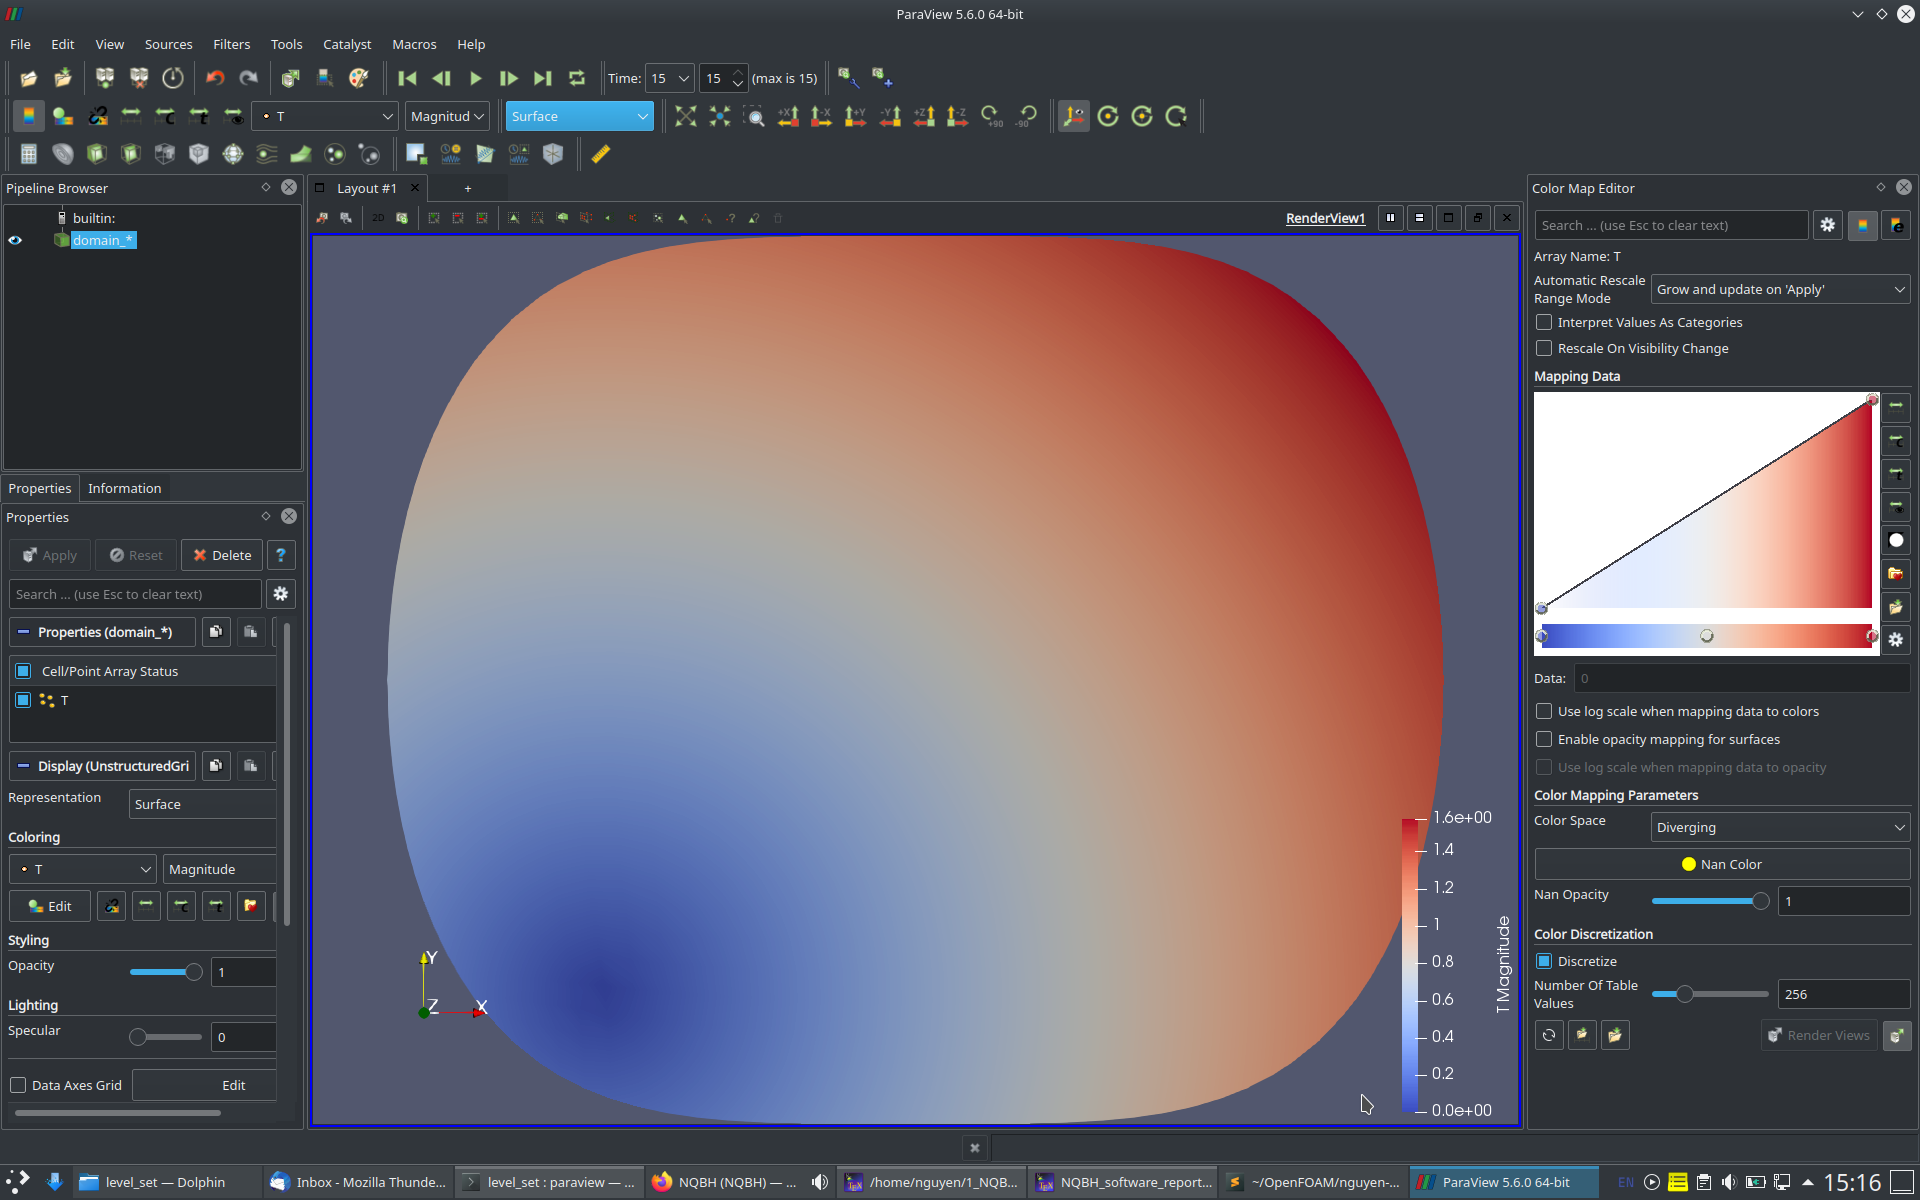
\includegraphics[height=0.44\textheight]{level_set_optimized_domain_after_15_steps_T_Surface}
            \caption{View the optimized domain after 15 optimization steps by ParaView with modes: \texttt{$T$, Surface}.}
        \end{figure}
        
        \begin{figure}[H]
            \centering
            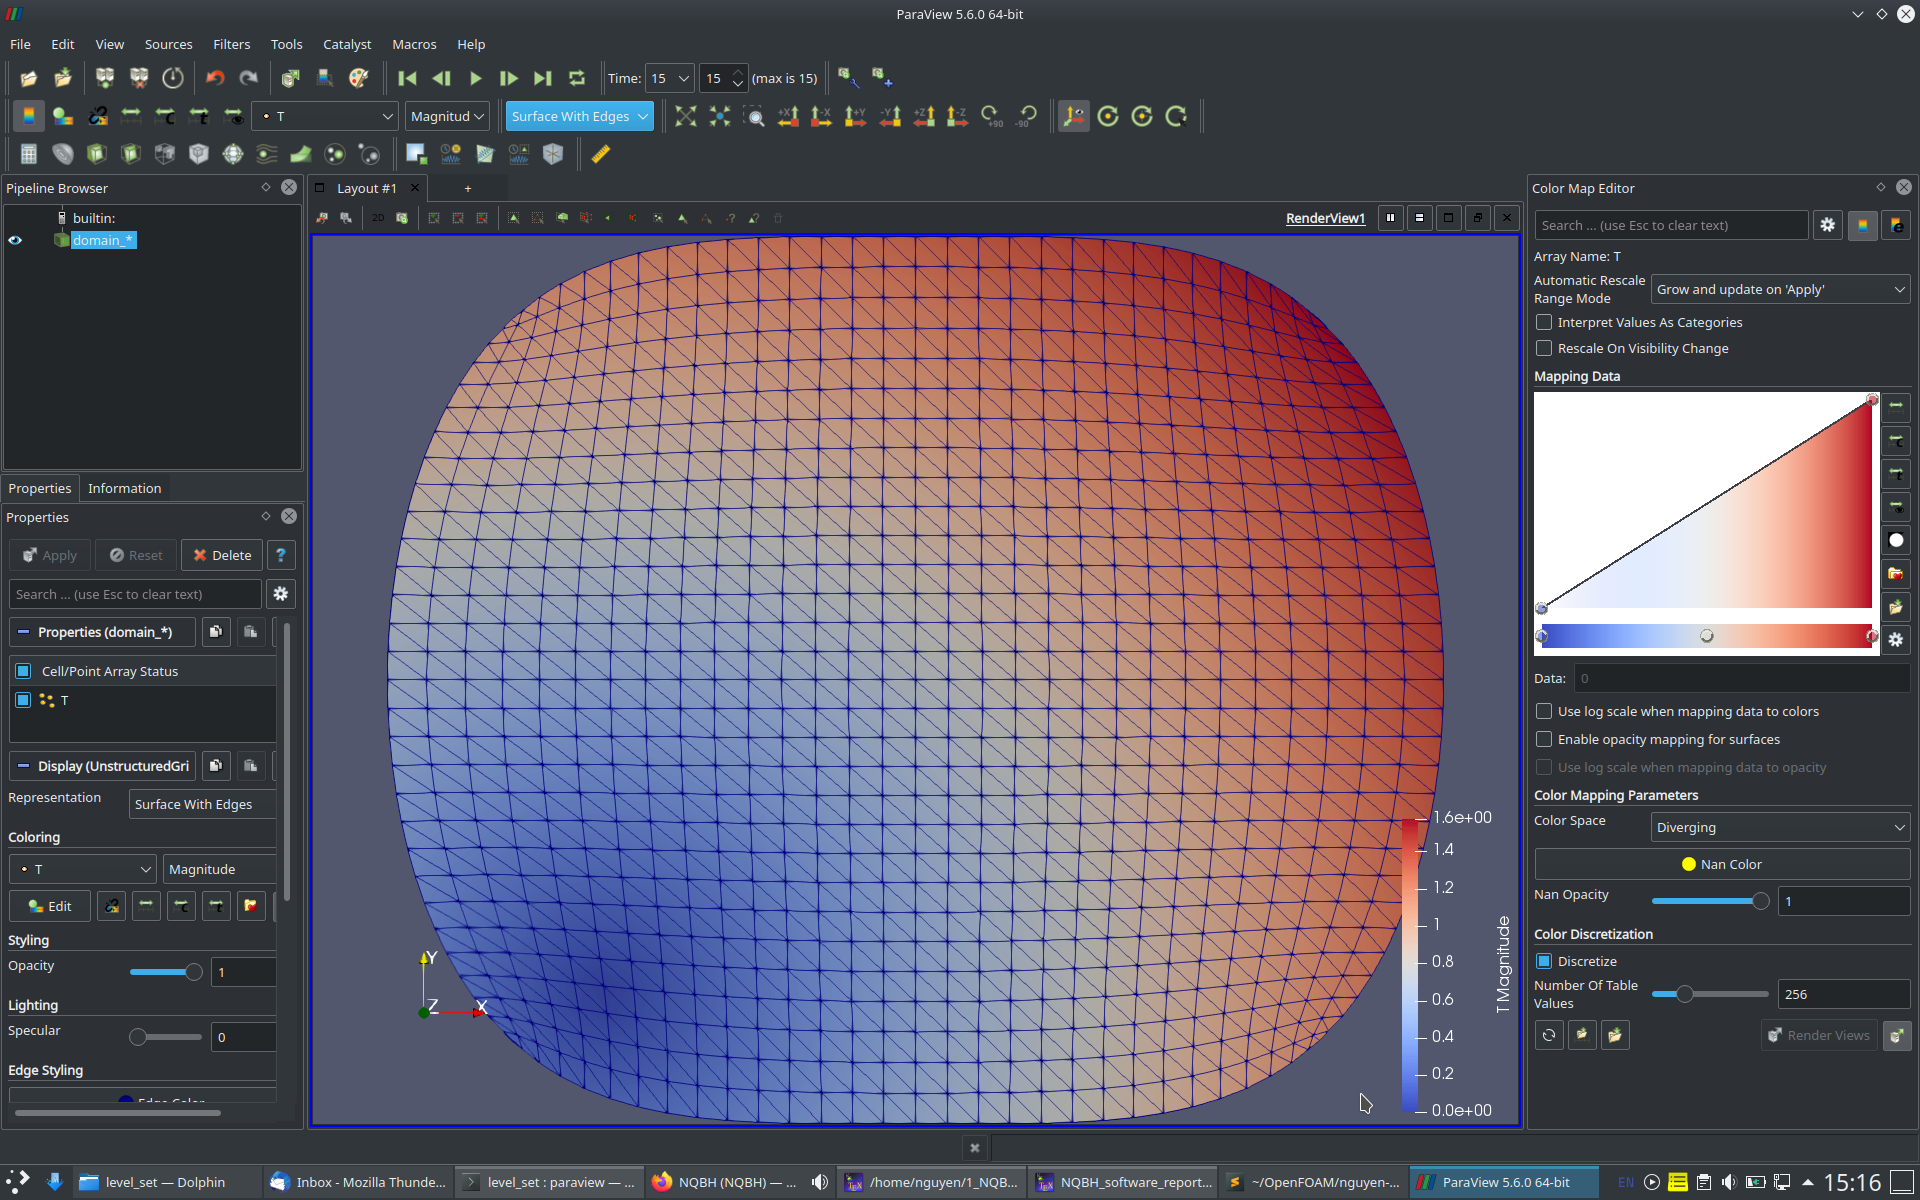
\includegraphics[height=0.44\textheight]{level_set_optimized_domain_after_15_steps_T_Surface_with_Edges}
            \caption{View the optimized domain after 15 optimization steps by ParaView with modes: \texttt{$T$, Surface with Edges}.}
        \end{figure}
        
        \item \href{https://fireshape.readthedocs.io/en/latest/example_L2tracking.html}{\textbf{Example 2: $L^2$-tracking}}: Minimize the shape functional
        \begin{equation*}
            J(\Omega) := \int_\Omega \left(u_({\bf x}) - u_t({\bf x})\right)^2{\rm d}{\bf x}, \mbox{ where } \left\{\begin{split}
                -\Delta u &= 4 &&\mbox{ in } \Omega,\\
                u &= 0 &&\mbox{ on } \partial\Omega,
            \end{split}\right.
        \end{equation*}
        and $u_t:\mathbb{R}^2\to\mathbb{R}$ is a target function:
        \begin{align*}
            u_t(x,y) = \frac{9}{25} - \left(x - \frac{1}{2}\right)^2 + \left(y - \frac{1}{2}\right)^2 - \frac{1}{2}.
        \end{align*}
        Optimal solution: $\emptyset$ and $\Omega_{\rm opt} := B_{3/5}((\frac{1}{2},\frac{1}{2}))$.
        
        \textbf{Numerical results.}
        
        \begin{figure}[H]
            \centering
            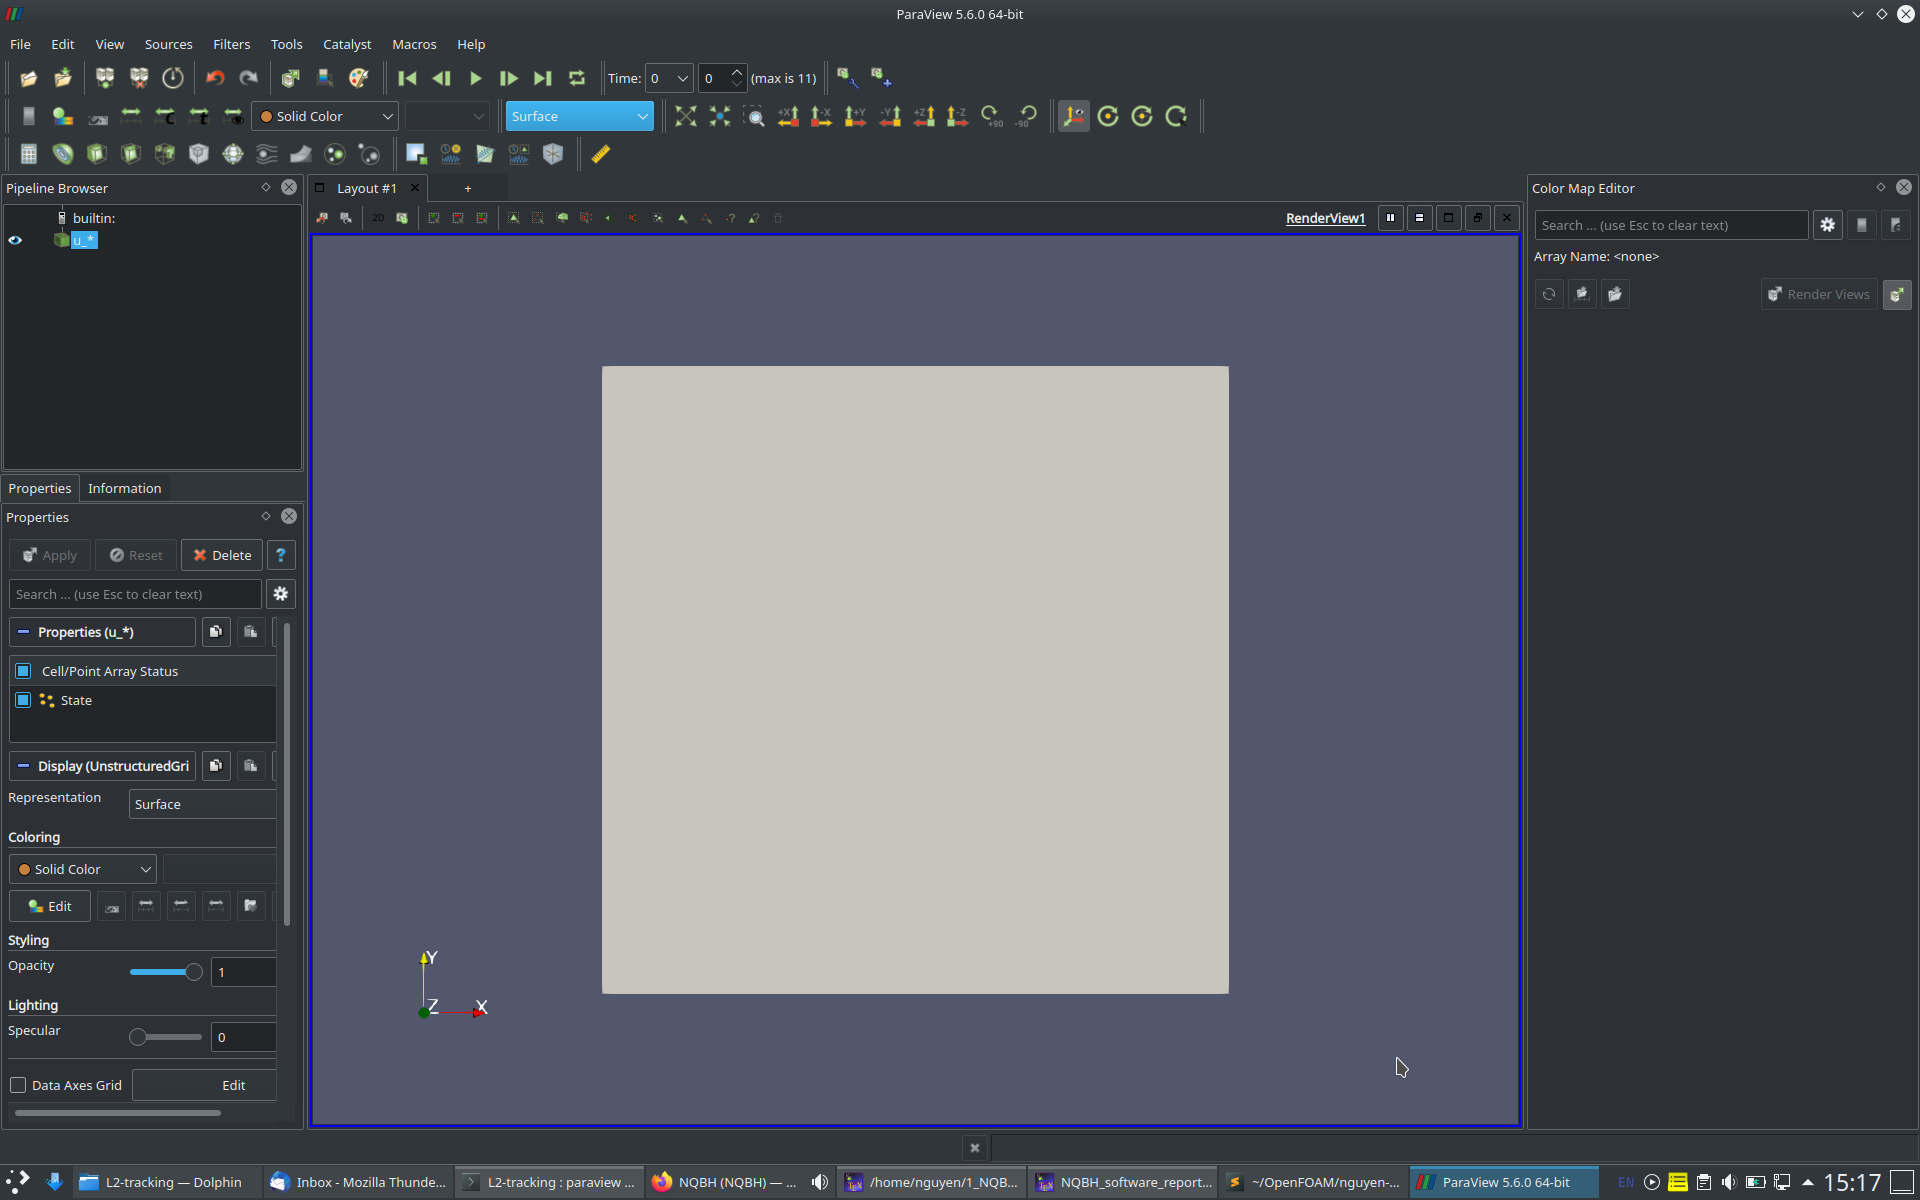
\includegraphics[height=0.44\textheight]{L2-tracking_initial_domain_Solid_Color_Surface}
            \caption{View the initial domain by ParaView with modes: \texttt{Solid Color, Surface}.}
        \end{figure}
        
        \begin{figure}[H]
            \centering
            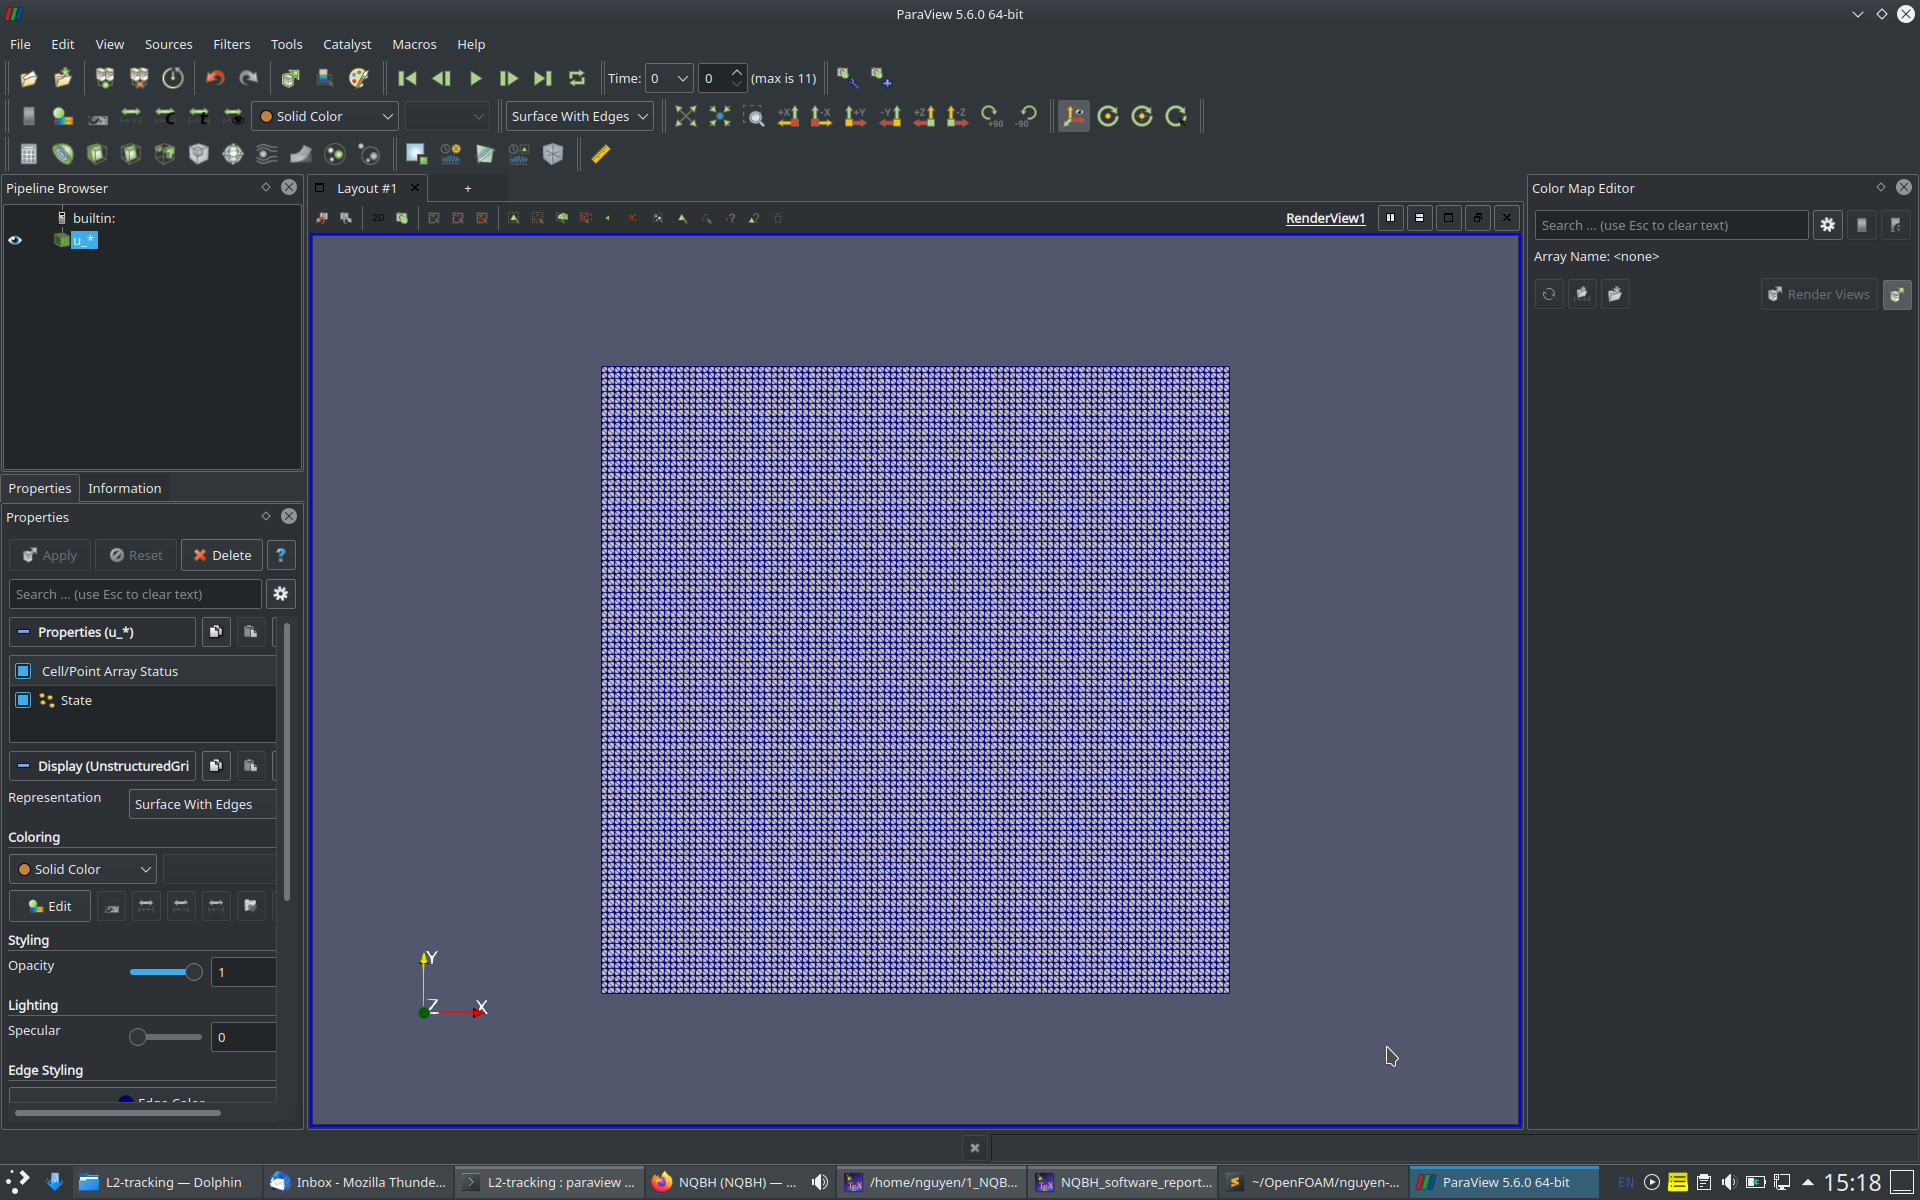
\includegraphics[height=0.44\textheight]{L2-tracking_initial_domain_Solid_Color_Surface_with_Edges}
            \caption{View the initial domain by ParaView with modes: \texttt{Solid Color, Surface with Edges}.}
        \end{figure}
    
        %
        \begin{figure}[H]
            \centering
            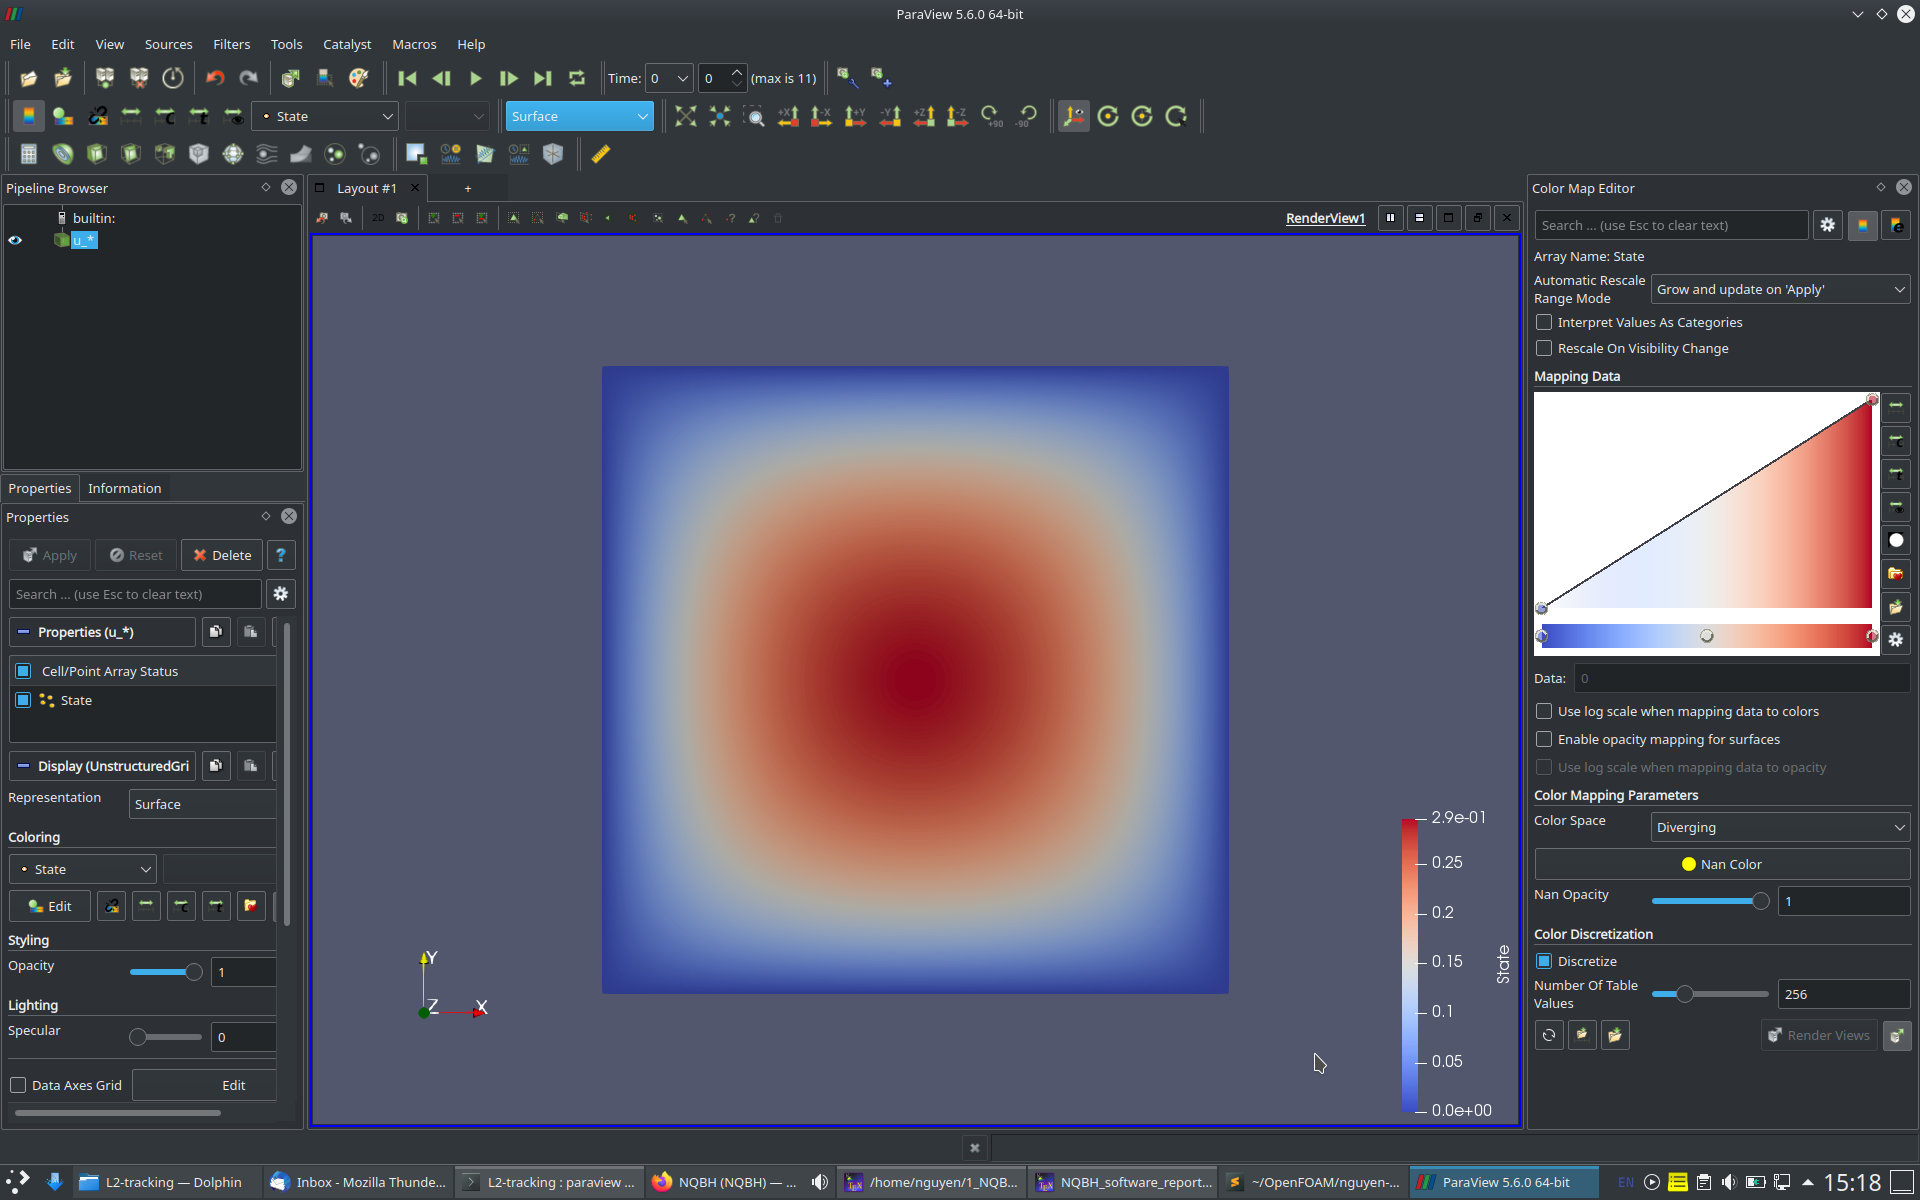
\includegraphics[height=0.44\textheight]{L2-tracking_initial_domain_State_Surface}
            \caption{View the initial domain by ParaView with modes: \texttt{State, Surface}.}
        \end{figure}
        
        \begin{figure}[H]
            \centering
            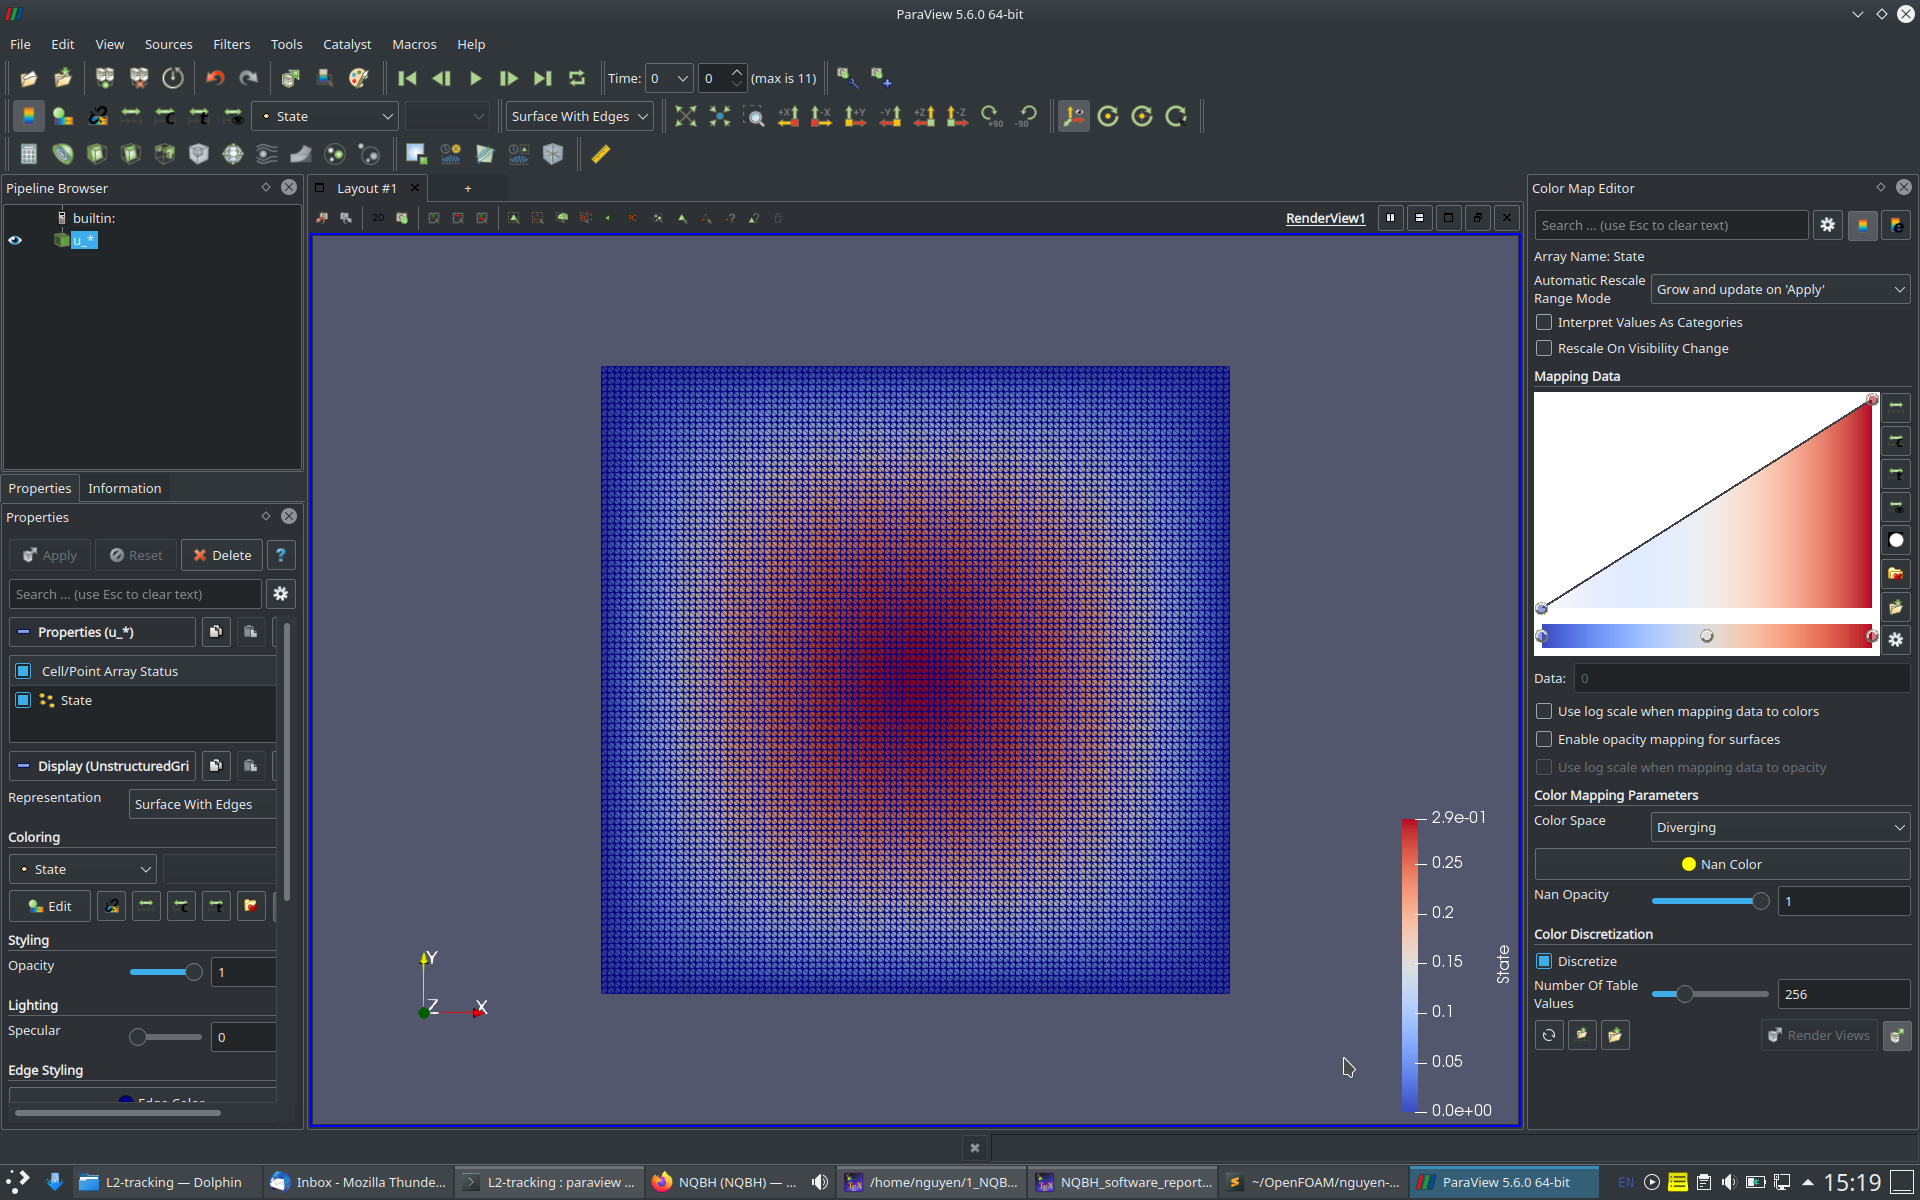
\includegraphics[height=0.44\textheight]{L2-tracking_initial_domain_State_Surface_with_Edges}
            \caption{View the initial domain by ParaView with modes: \texttt{State, Surface with Edges}.}
        \end{figure}

        %
        \begin{figure}[H]
            \centering
            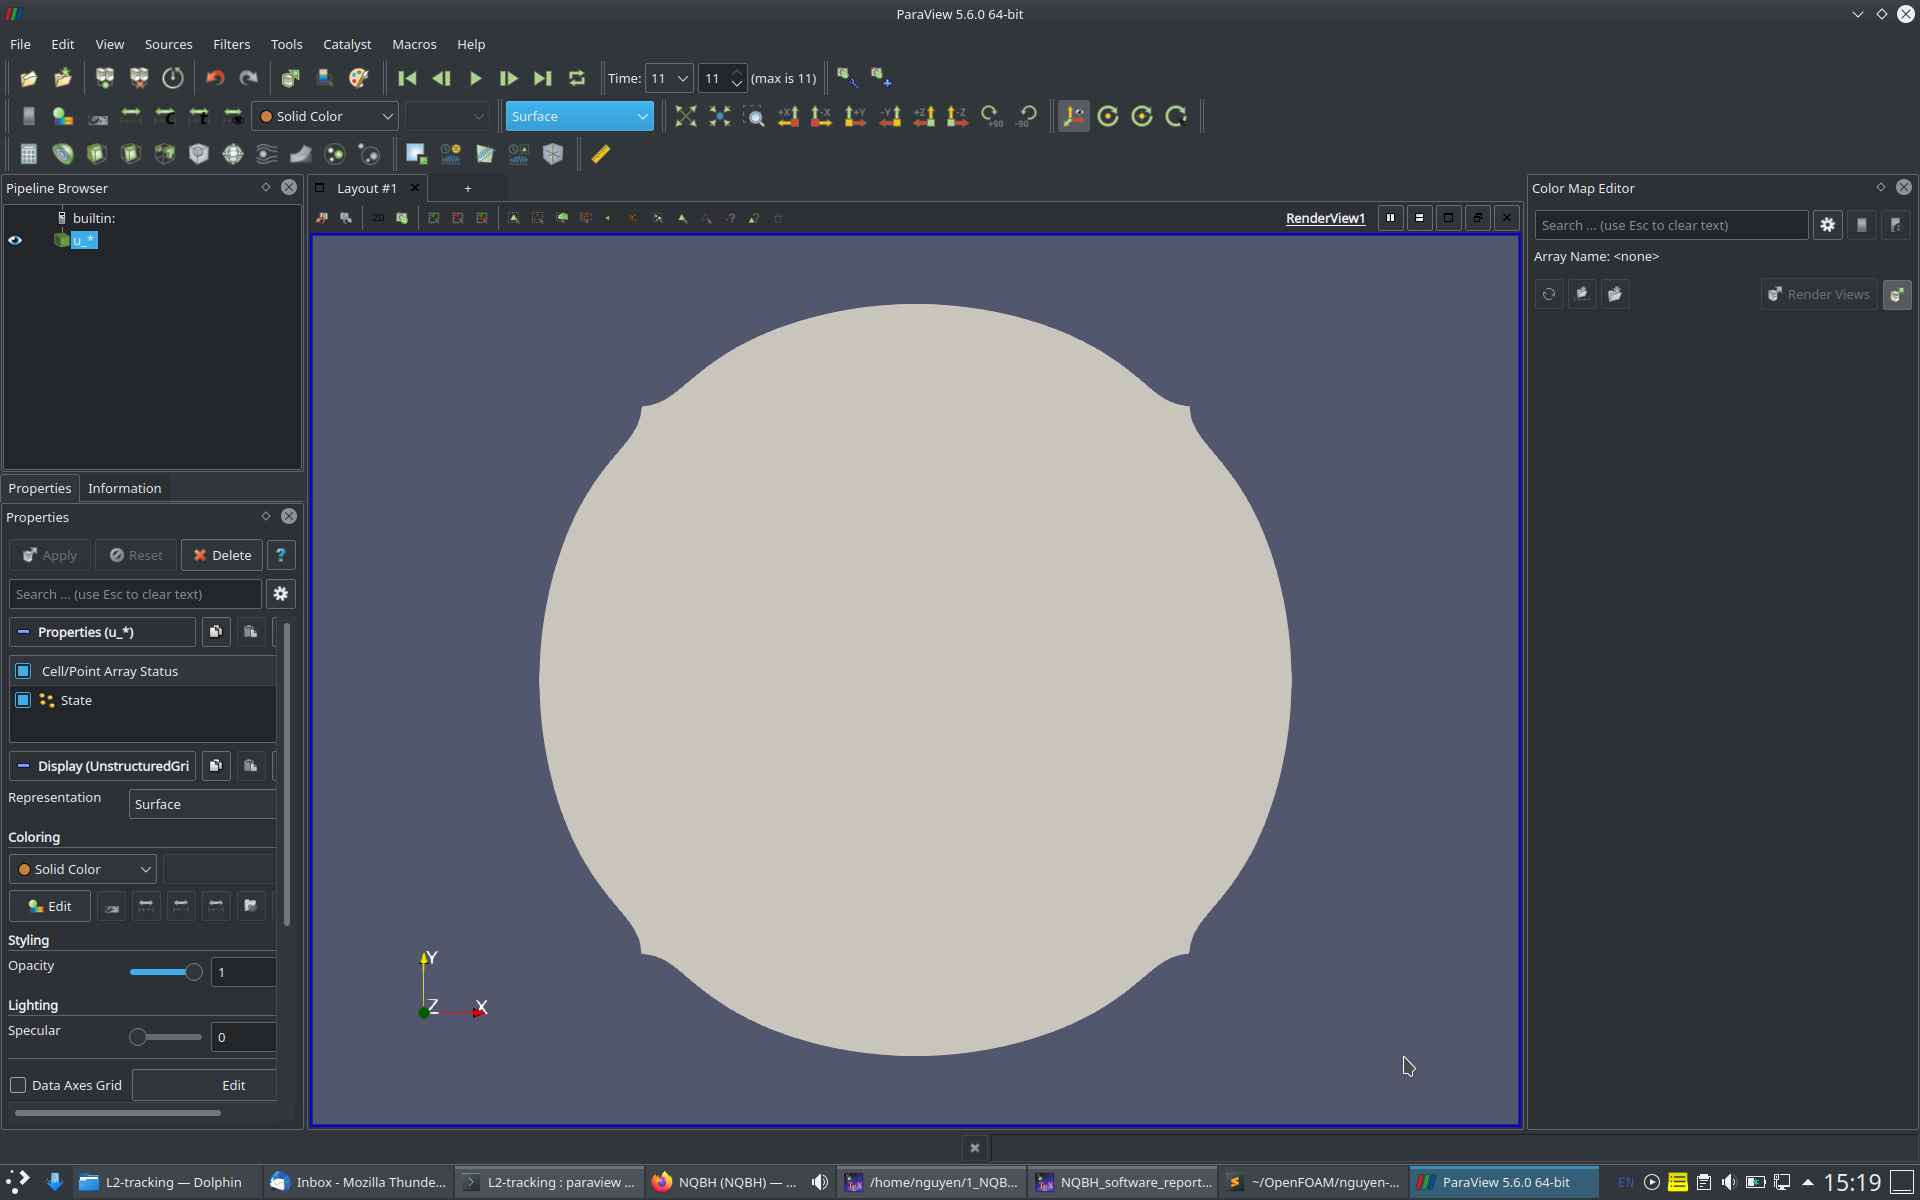
\includegraphics[height=0.44\textheight]{L2-tracking_optimized_domain_after_11_steps_Solid_Color_Surface}
            \caption{View the optimized domain after 11 optimization steps by ParaView with modes: \texttt{Solid Color, Surface}.}
        \end{figure}
        
        \begin{figure}[H]
            \centering
            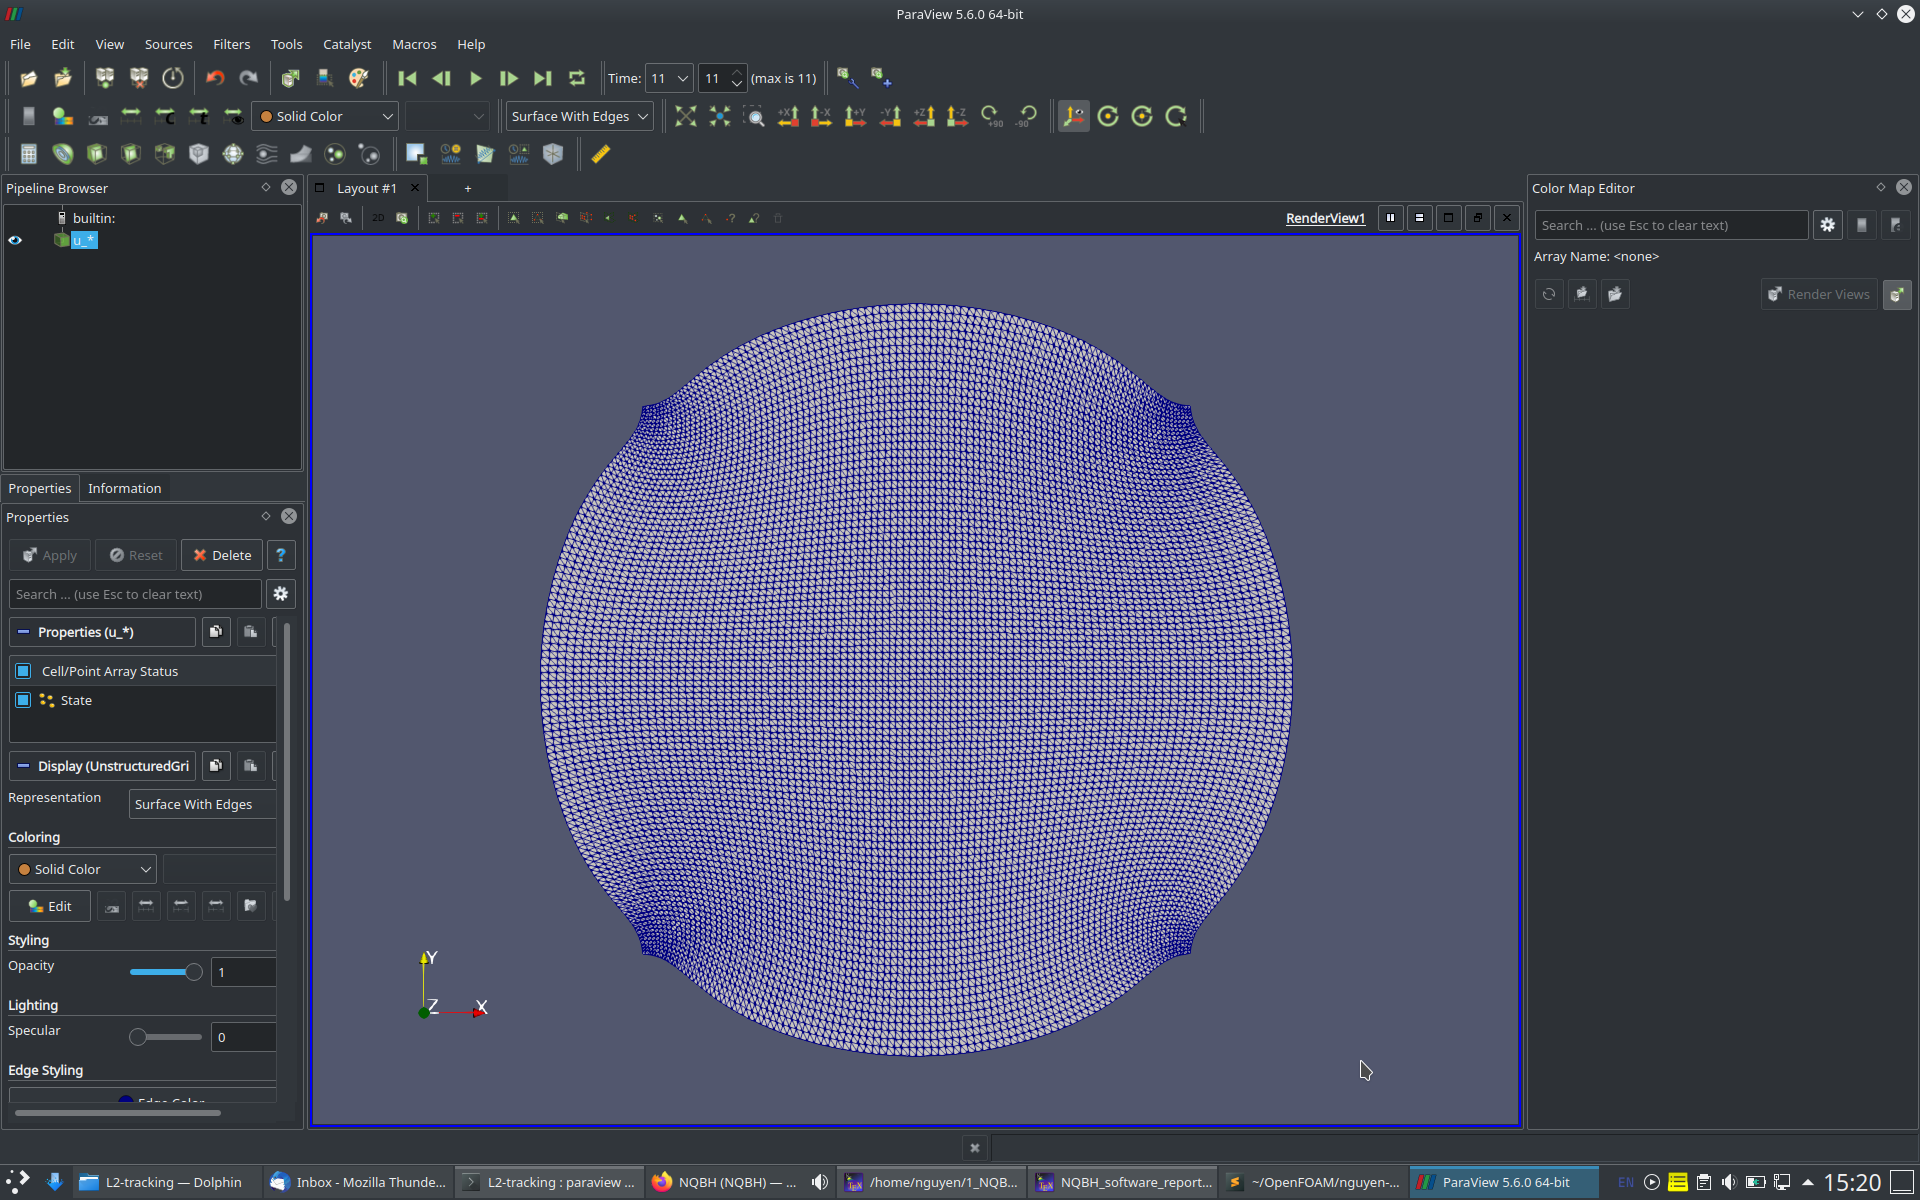
\includegraphics[height=0.44\textheight]{L2-tracking_optimized_domain_after_11_steps_Solid_Color_Surface_with_Edges}
            \caption{View the optimized domain after 11 optimization steps by ParaView with modes: \texttt{Solid Color, Surface with Edges}.}
        \end{figure}
    
        %
        \begin{figure}[H]
            \centering
            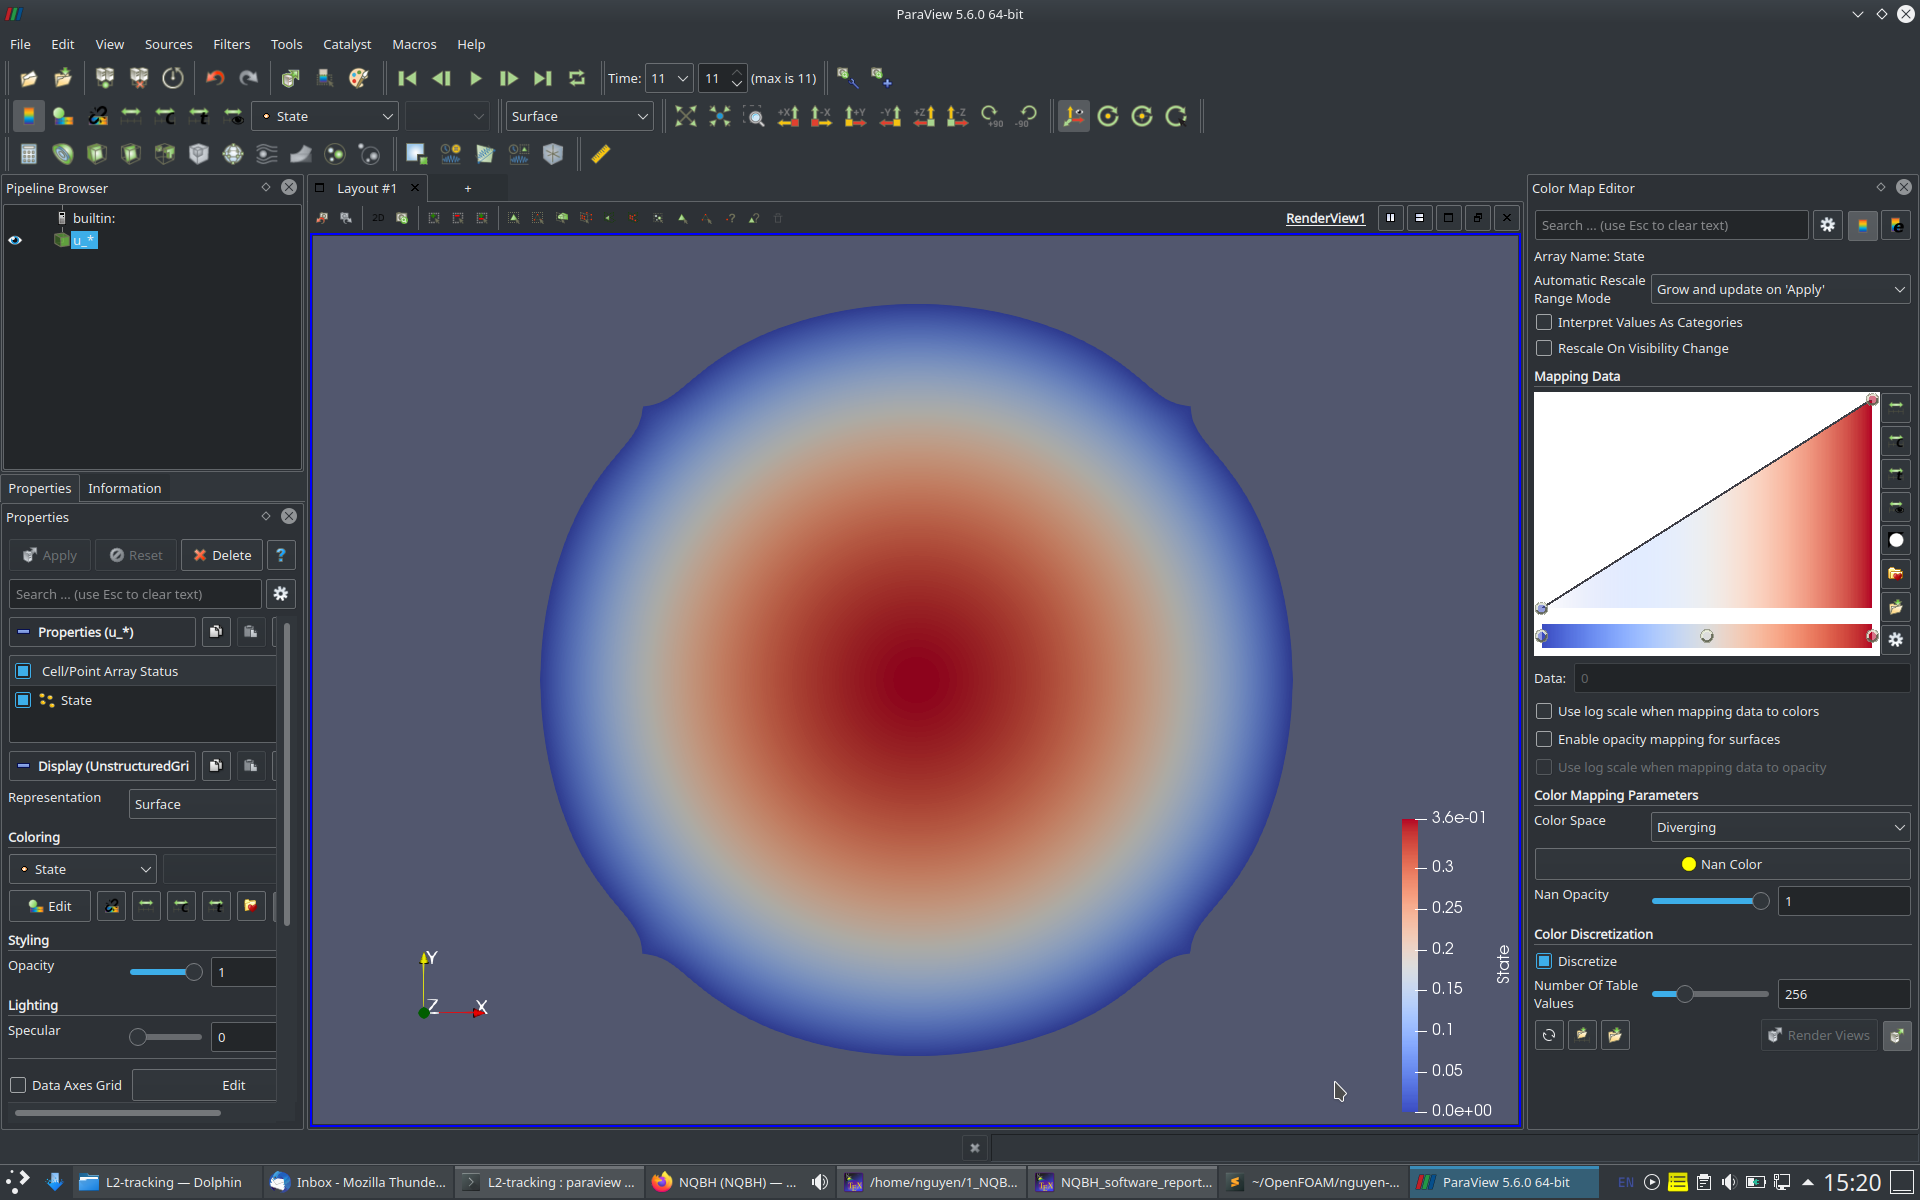
\includegraphics[height=0.44\textheight]{L2-tracking_optimized_domain_after_11_steps_State_Surface}
            \caption{View the optimized domain after 11 optimization steps by ParaView with modes: \texttt{State, Surface}.}
        \end{figure}
        
        \begin{figure}[H]
            \centering
            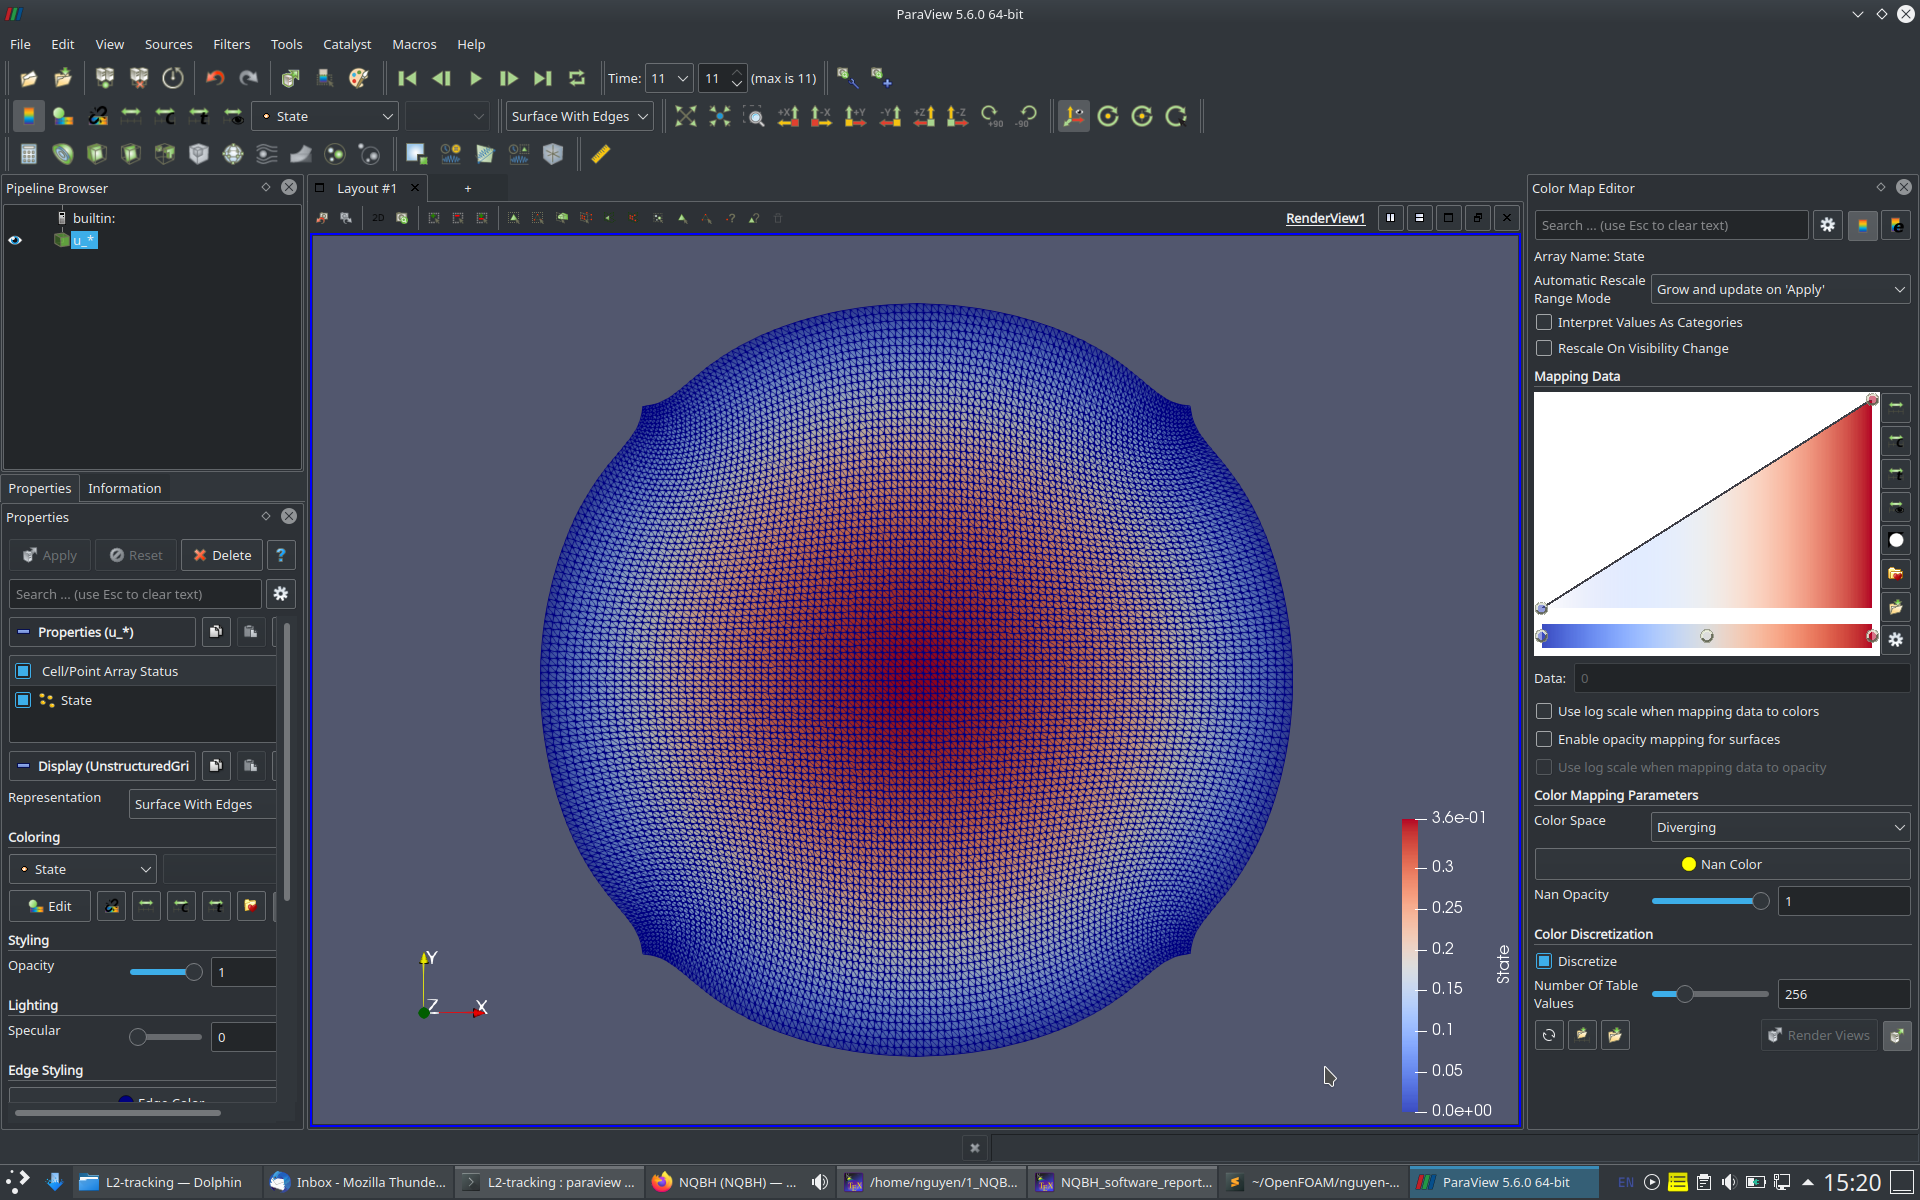
\includegraphics[height=0.44\textheight]{L2-tracking_optimized_domain_after_11_steps_State_Surface_with_Edges}
            \caption{View the optimized domain after 11 optimization steps by ParaView with modes: \texttt{State, Surface with Edges}.}
        \end{figure}    
    
        \item \href{https://fireshape.readthedocs.io/en/latest/example_pipe.html}{\textbf{Example 3: Kinetic energy dissipation in a pipe}}: Minimize the shape functional:
        \begin{align*}
            J(\Omega) = \int_\Omega \nu\nabla{\bf u}:\nabla{\bf u}{\rm d}{\bf x},
        \end{align*}
        where the fluid velocity ${\bf u}:\mathbb{R}^d\to\mathbb{R}^d$ and the fluid pressure $p:\mathbb{R}^d\to\mathbb{R}$, $d\in\{2,3\}$ satisfy the incompressible Navier-Stokes equations
        \begin{equation*}
            \left\{\begin{split}
                -\nu\Delta{\bf u} + ({\bf u}\cdot\nabla){\bf u} + \nabla p &= {\bf 0} &&\mbox{ in } \Omega,\\
                \nabla\cdot{\bf u} &= 0 &&\mbox{ in } \Omega,\\
                {\bf u} &= {\bf g} &&\mbox{ on } \partial\Omega\backslash\Gamma_{\rm out},\\
                p{\bf n} - \nu\nabla{\bf u}\cdot{\bf n} &= {\bf 0} &&\mbox{ on } \Gamma_{\rm out},
            \end{split}\right.
        \end{equation*}
        where ${\bf g}$ is given by a Poiseuille flow at the inlet and is zero on the walls of the pipe.
        
        In addition to the PDE-constraint, enforce a \textit{volume constraint}: the volume of the optimized domain should be equal to the volume of the initial domain: $\operatorname{Vol}(\Omega) = \operatorname{Vol}(\Omega_0) =: V_0$.
        
        \textbf{Numerical results.}
        \begin{itemize}
            \item \textbf{Architecture.} Dell Intel i5, Ubuntu 18.04.4 installed on VirtualBox host machine installed on a host machine installed Ubuntu 20.04.
            \item \textbf{Runtime.} $\approx$ 45 minutes.
        \end{itemize}
    
        $\star$ \textbf{2D.}
    
        \begin{figure}[H]
            \centering
            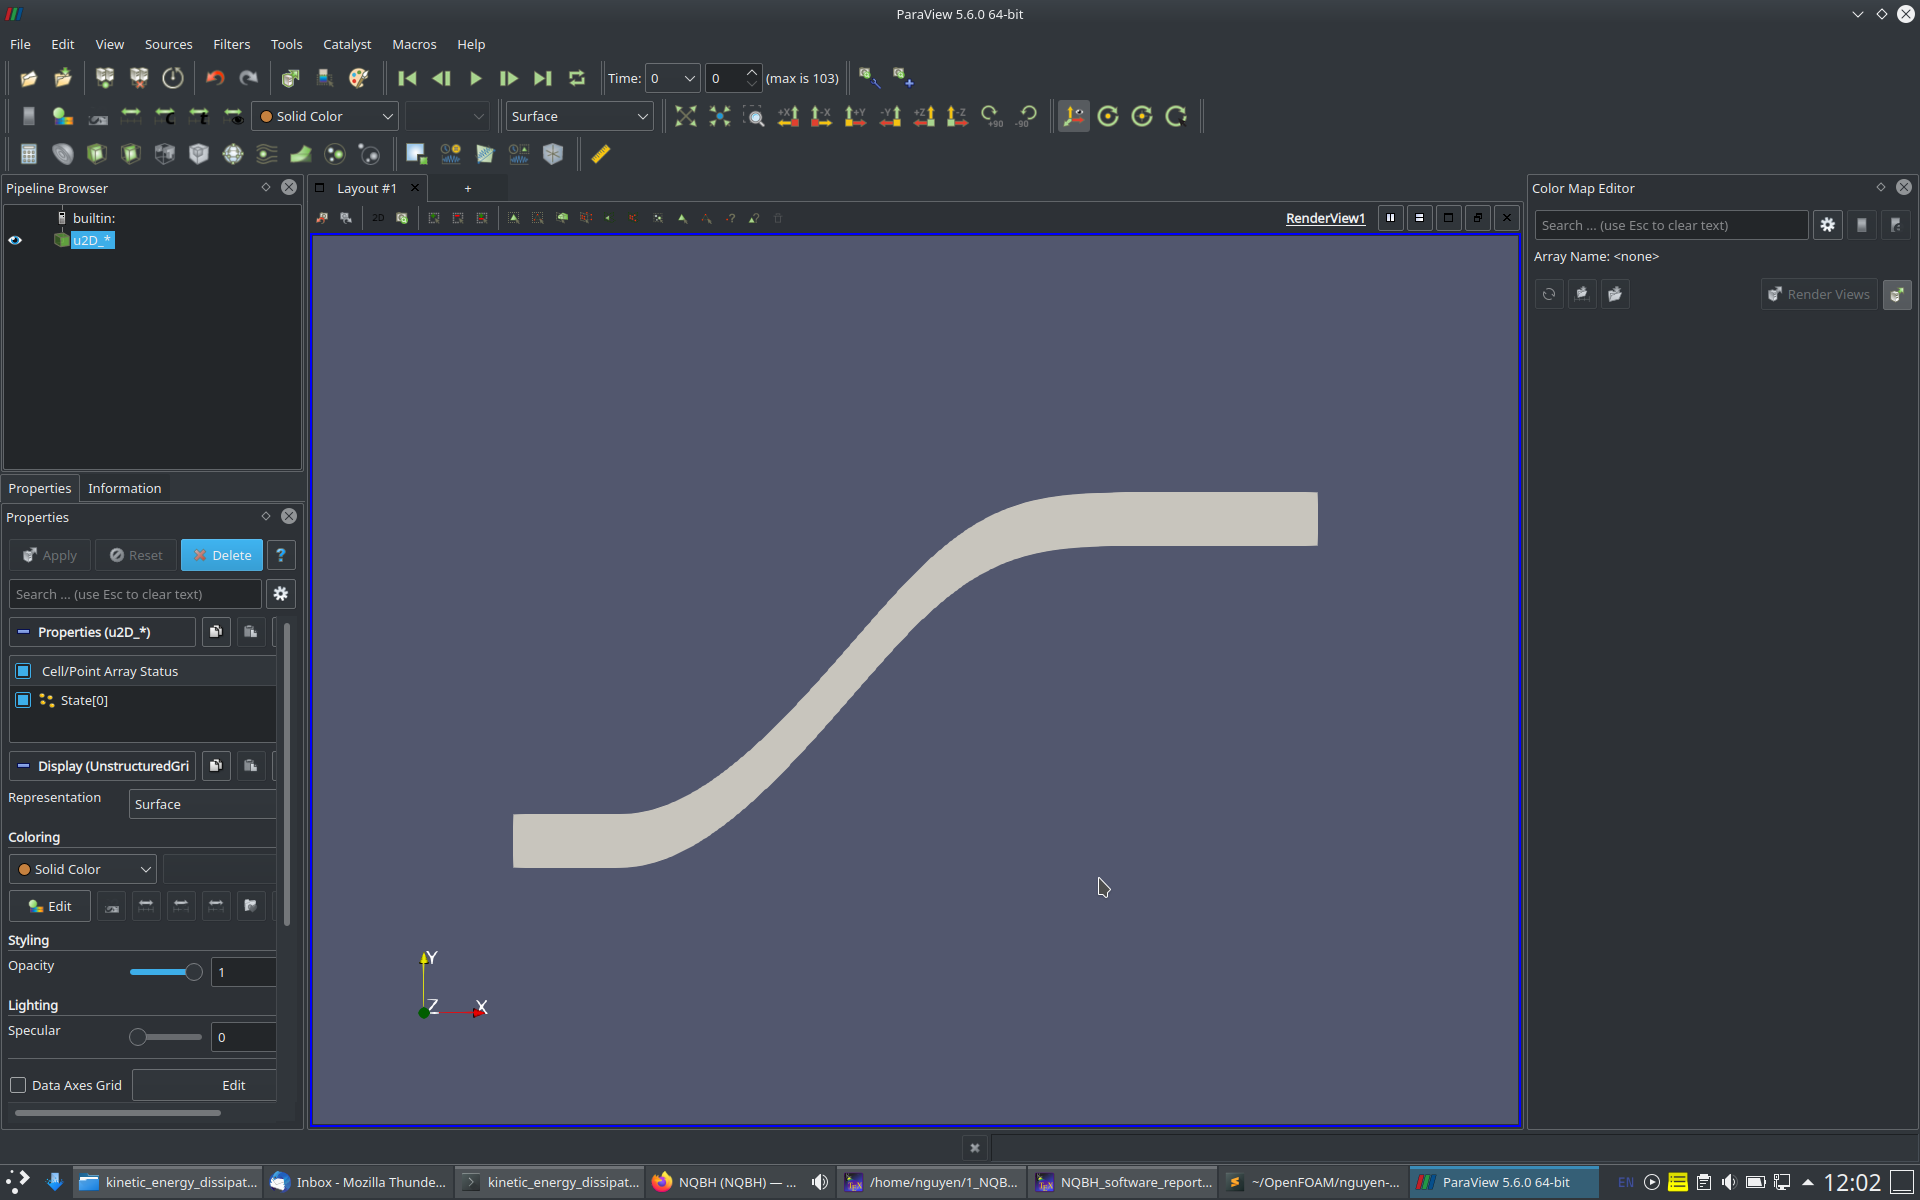
\includegraphics[height=0.44\textheight]{initial_domain_2D_Solid_Color_Surface}
            \caption{View the initial 2D domain in by ParaView with modes: \texttt{Solid Color, Surface}.}
        \end{figure}
        
        \begin{figure}[H]
            \centering
            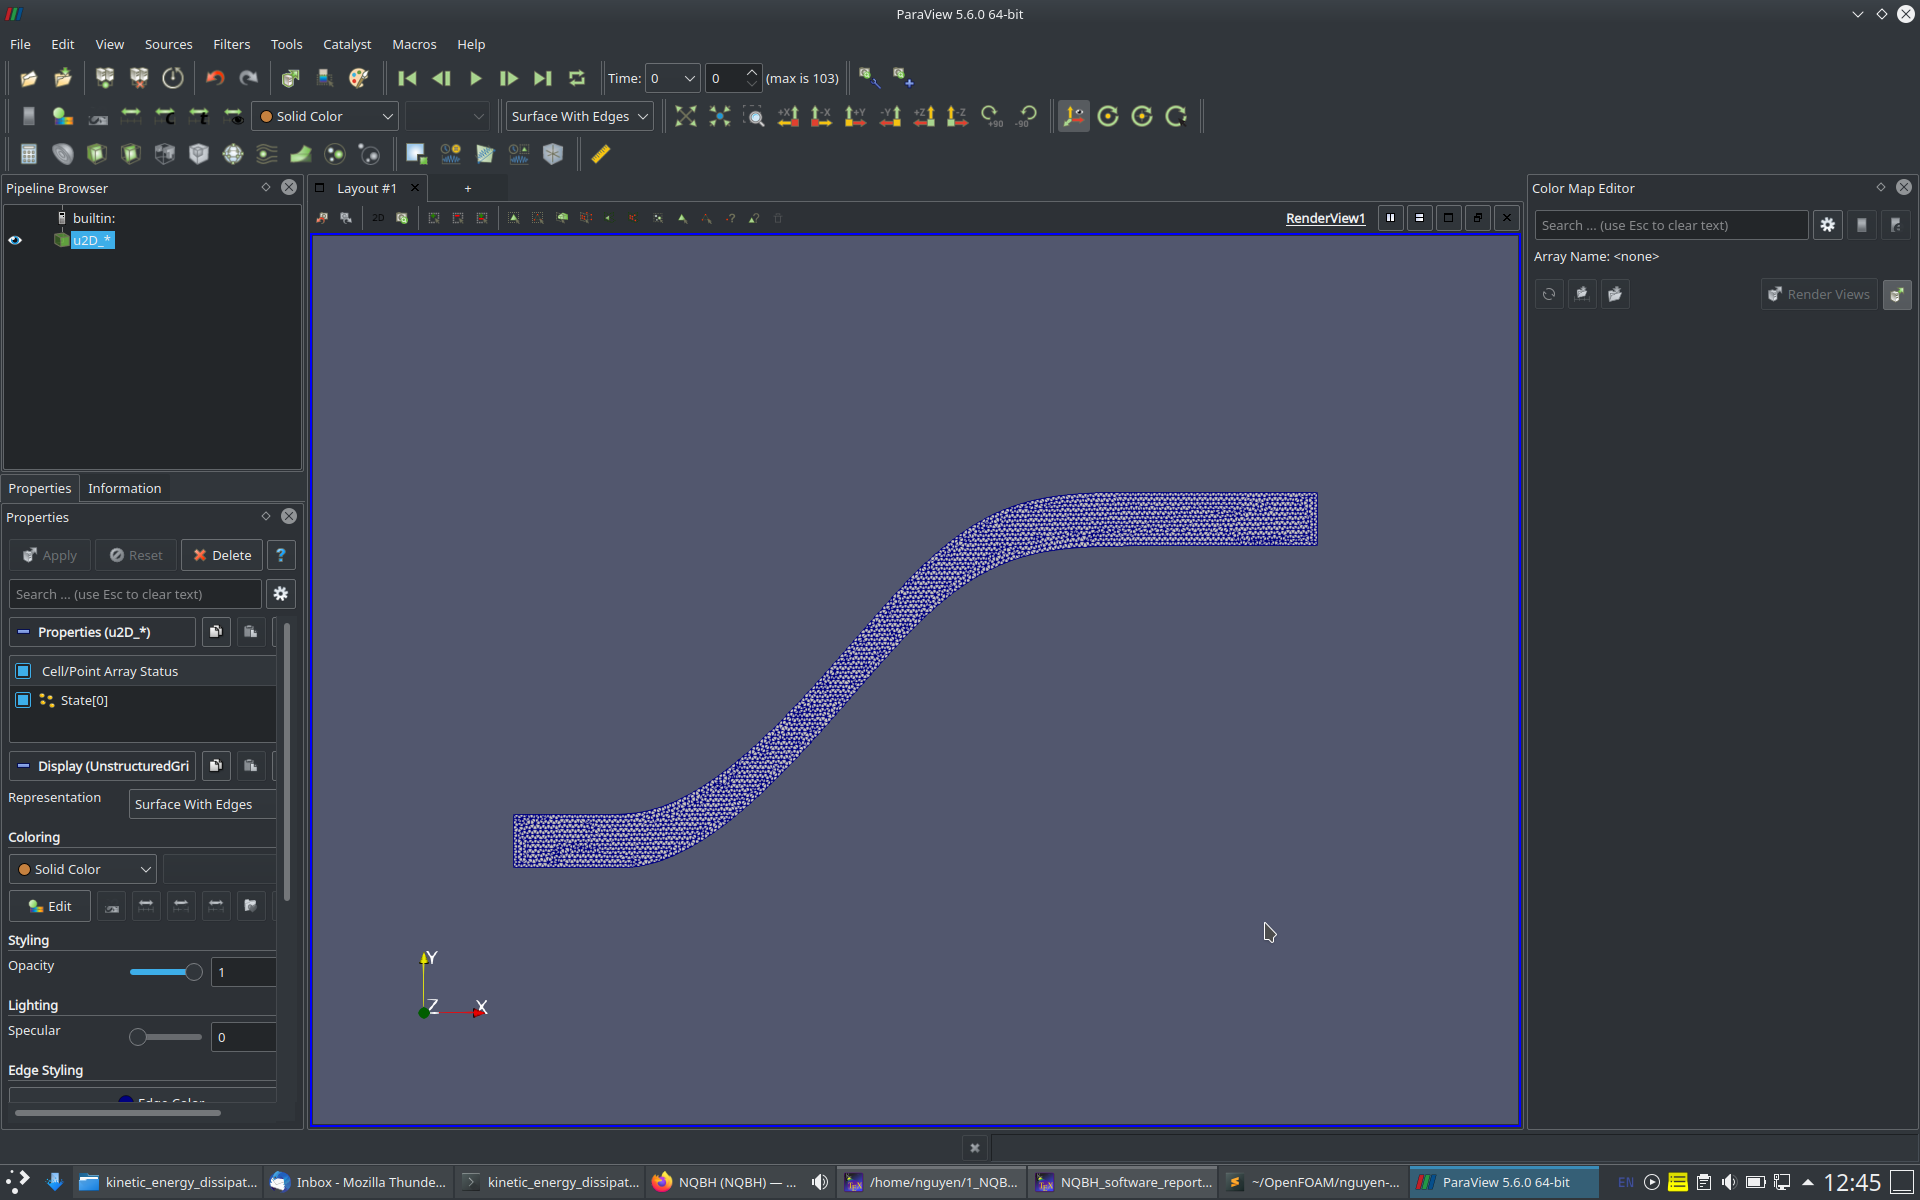
\includegraphics[height=0.44\textheight]{initial_domain_2D_Solid_Color_Surface_with_Edges}
            \caption{View the initial 2D domain by ParaView with modes: \texttt{Solid Color, Surface with Edges}.}
        \end{figure}
        
        %
        \begin{figure}[H]
            \centering
            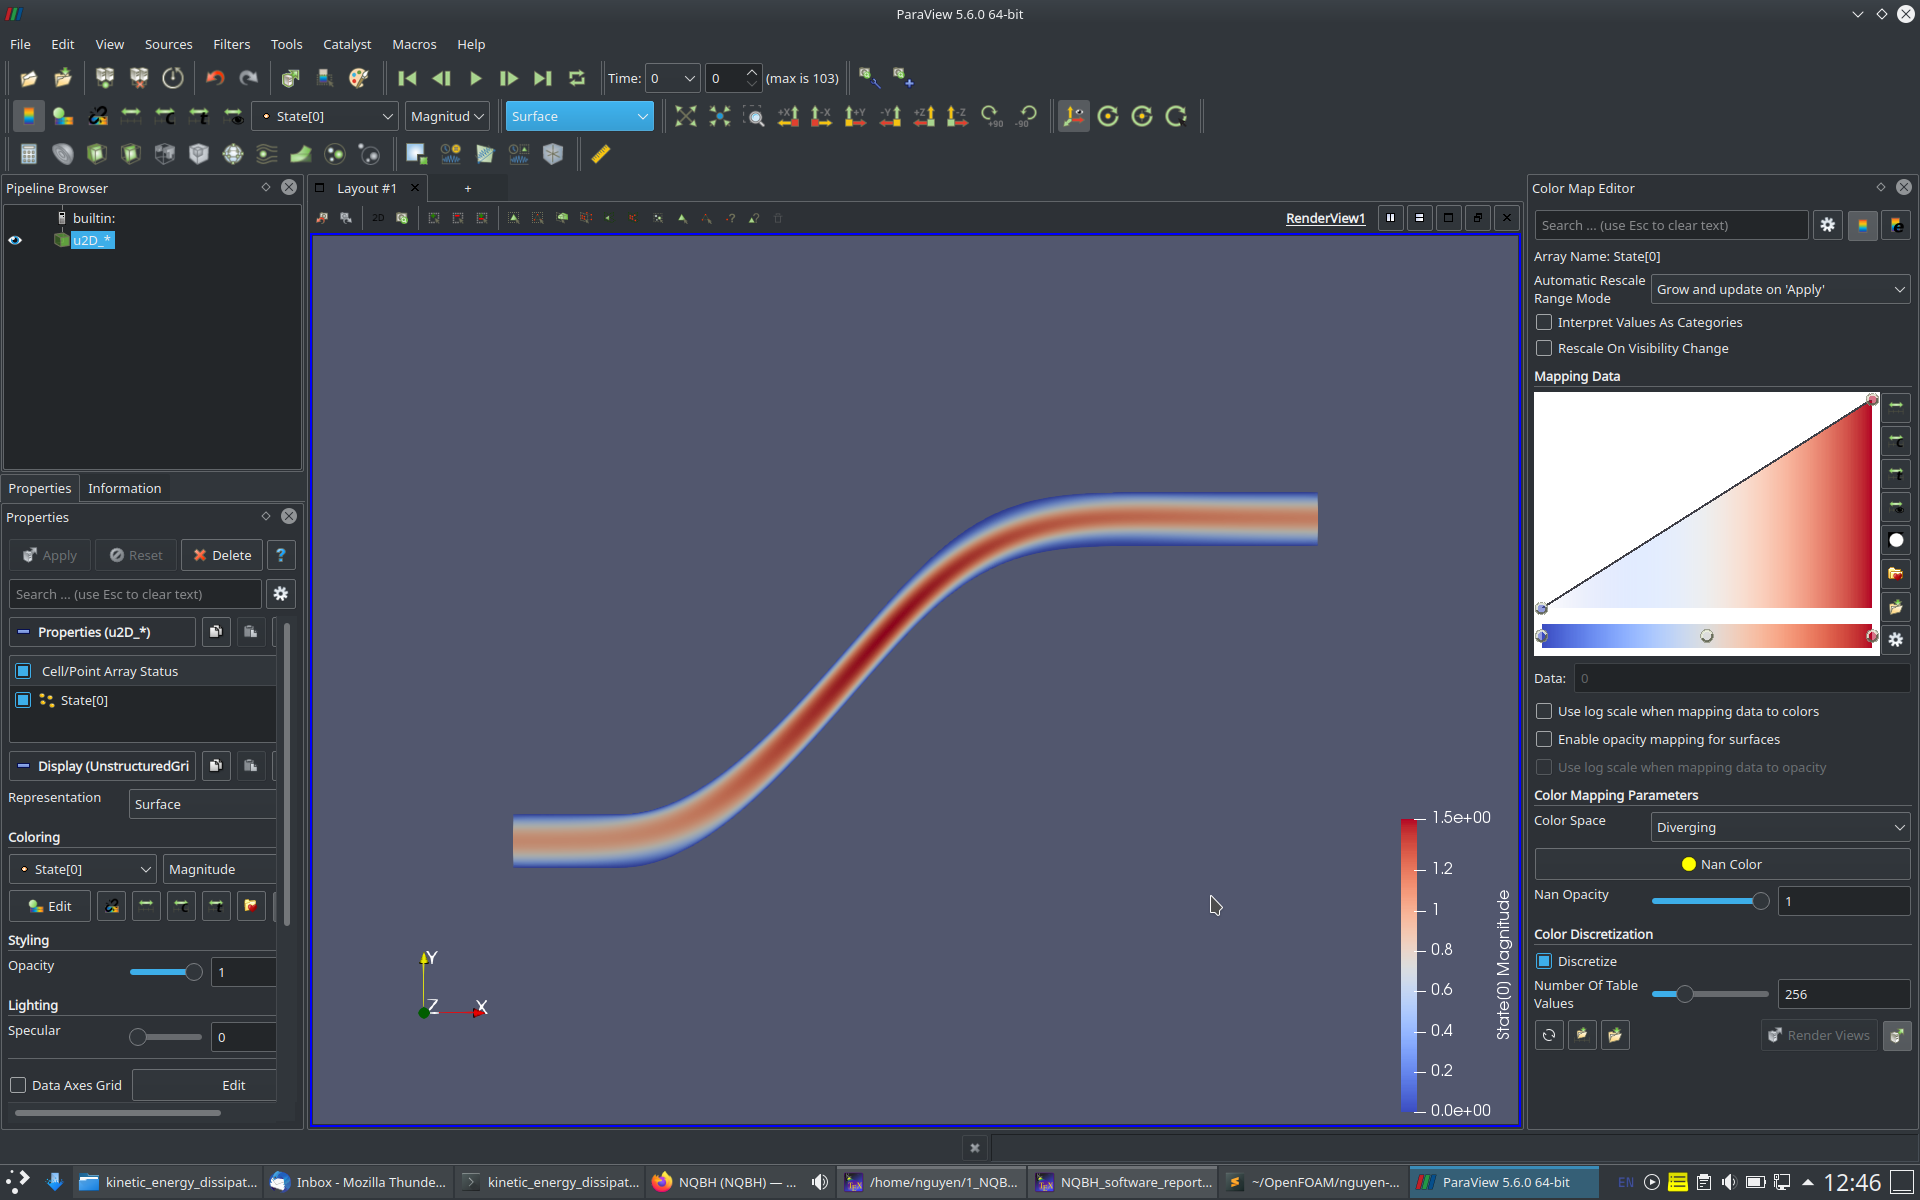
\includegraphics[height=0.44\textheight]{initial_domain_2D_State0_Surface}
            \caption{View the initial 2D domain by ParaView with modes: \texttt{State[0], Surface}.}
        \end{figure}
        
        \begin{figure}[H]
            \centering
            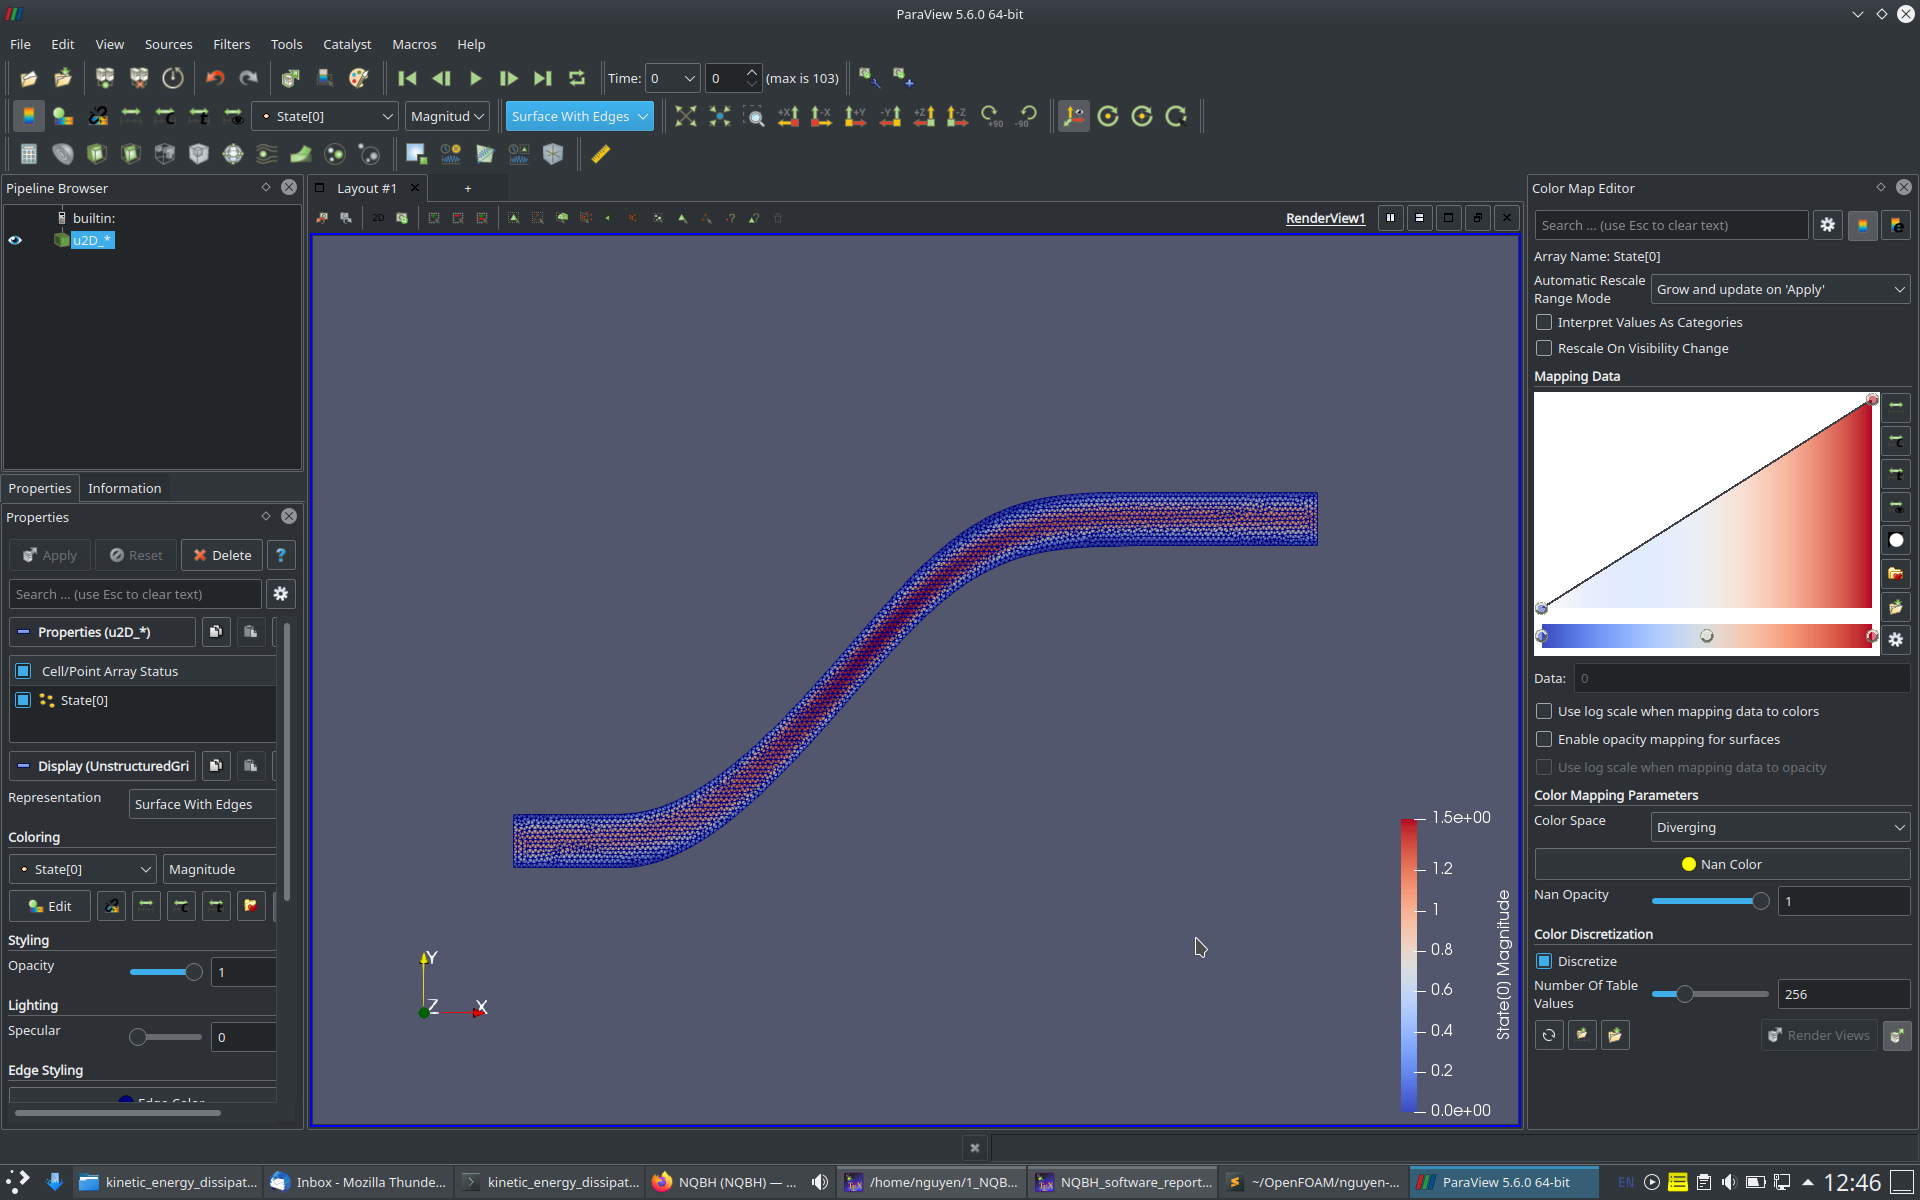
\includegraphics[height=0.44\textheight]{initial_domain_2D_State0_Surface_with_Edges}
            \caption{View the initial 2D domain by ParaView with modes: \texttt{State[0], Surface with Edges}.}
        \end{figure}
        
        %
        \begin{figure}[H]
            \centering
            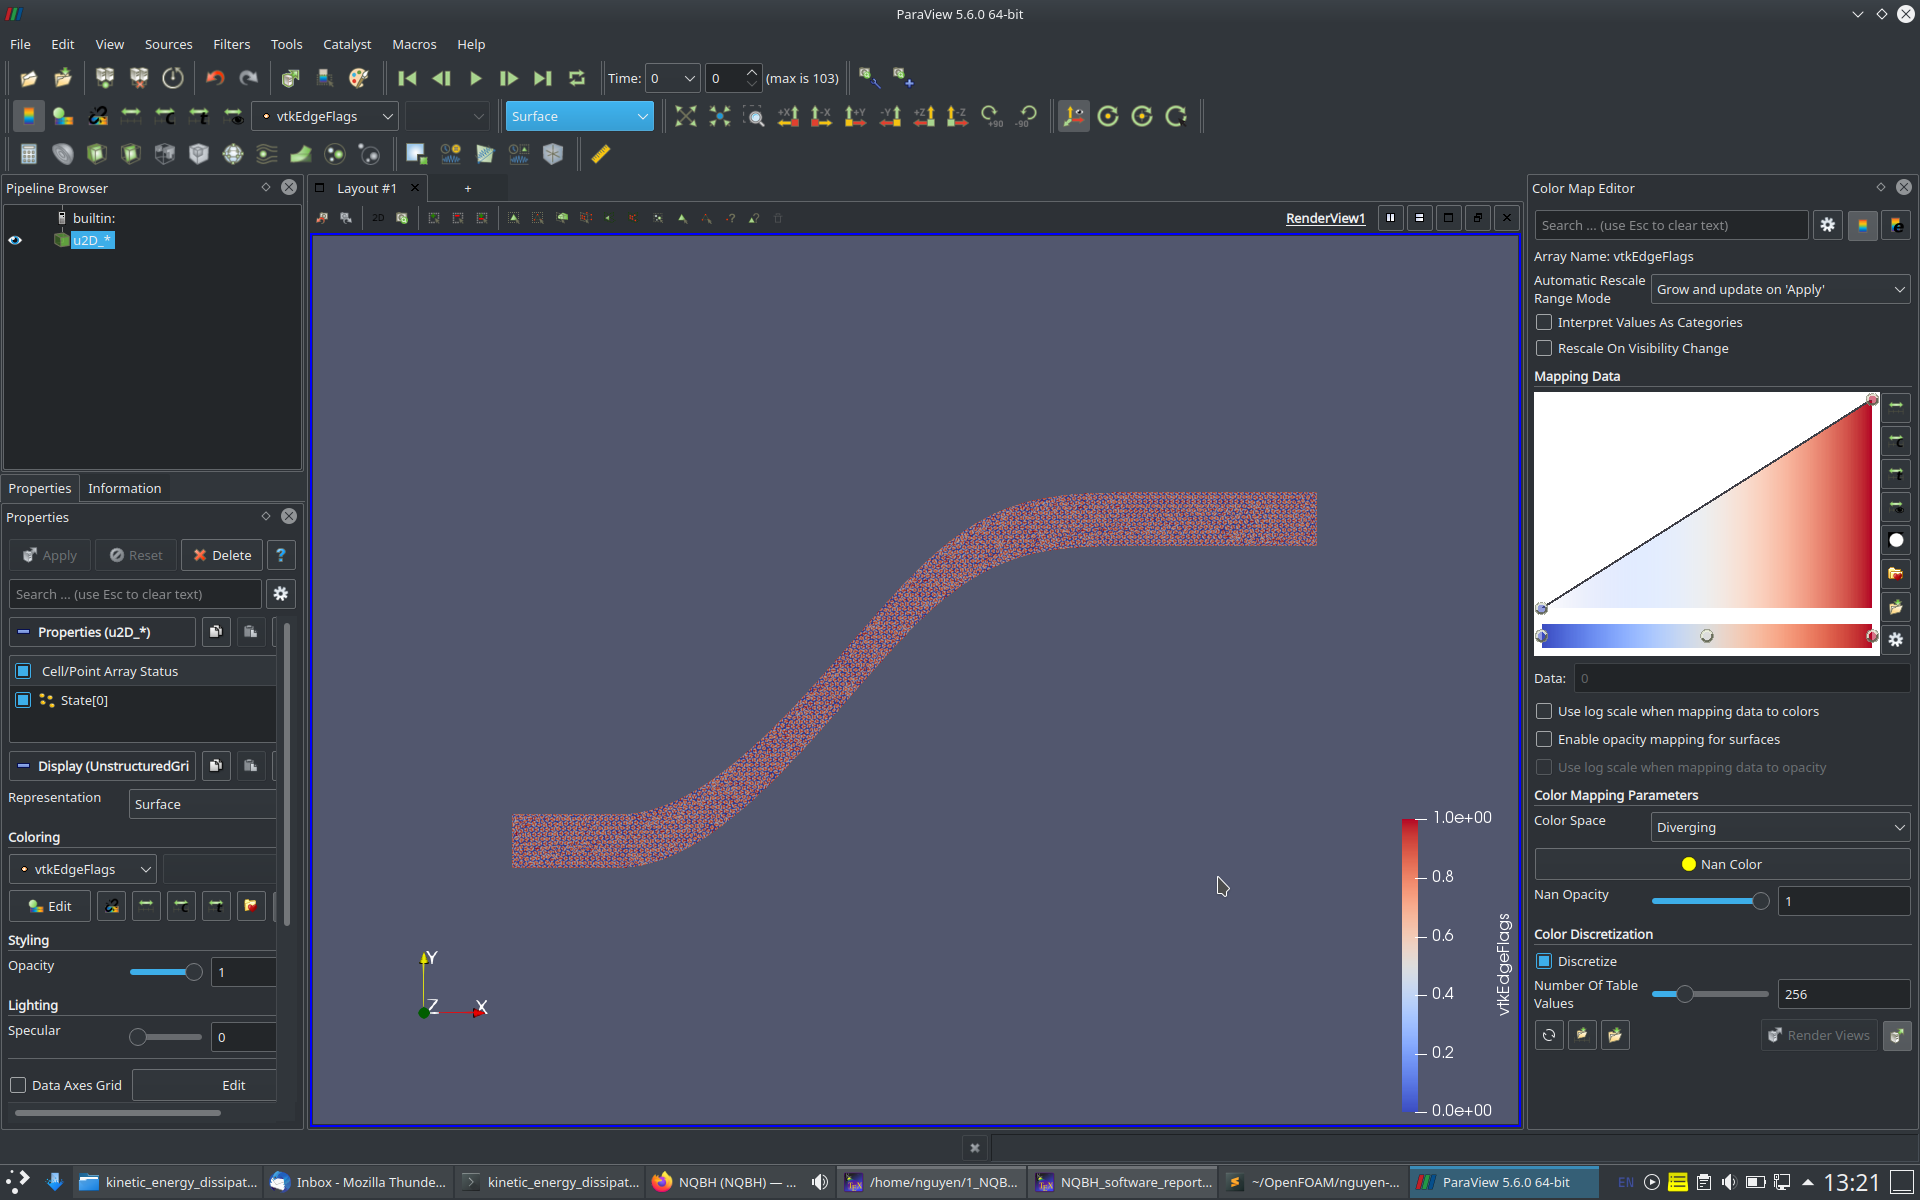
\includegraphics[height=0.44\textheight]{initial_domain_2D_vtkEdgeFlags_Surface}
            \caption{View the initial 2D domain by ParaView with modes: \texttt{vtkEdgeFlags, Surface}.}
        \end{figure}
        
        \begin{figure}[H]
            \centering
            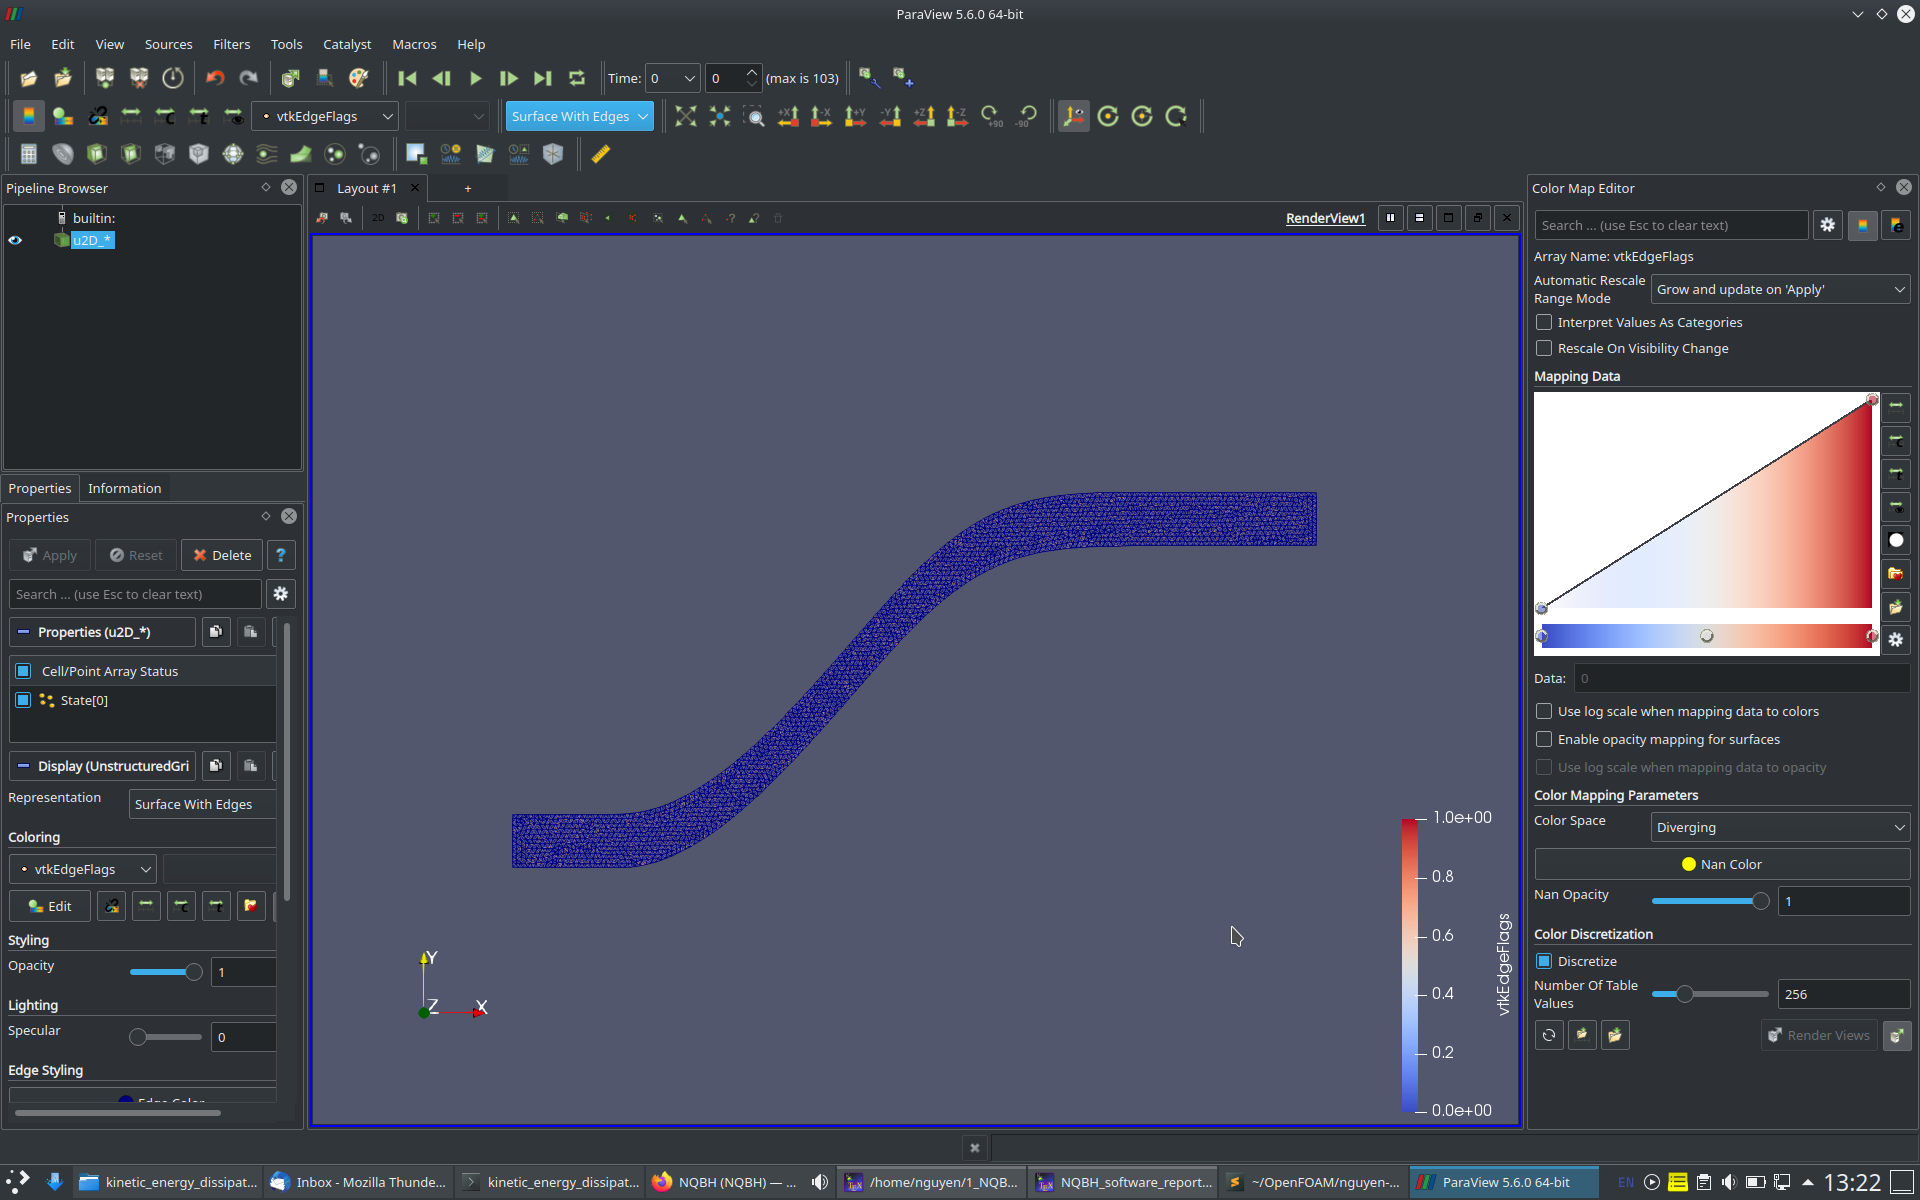
\includegraphics[height=0.44\textheight]{initial_domain_2D_vtkEdgeFlags_Surface_with_Edges}
            \caption{View the initial 2D domain by ParaView with modes: \texttt{vtkEdgeFlags, Surface with Edges}.}
        \end{figure}
        
        %
        \begin{figure}[H]
            \centering
            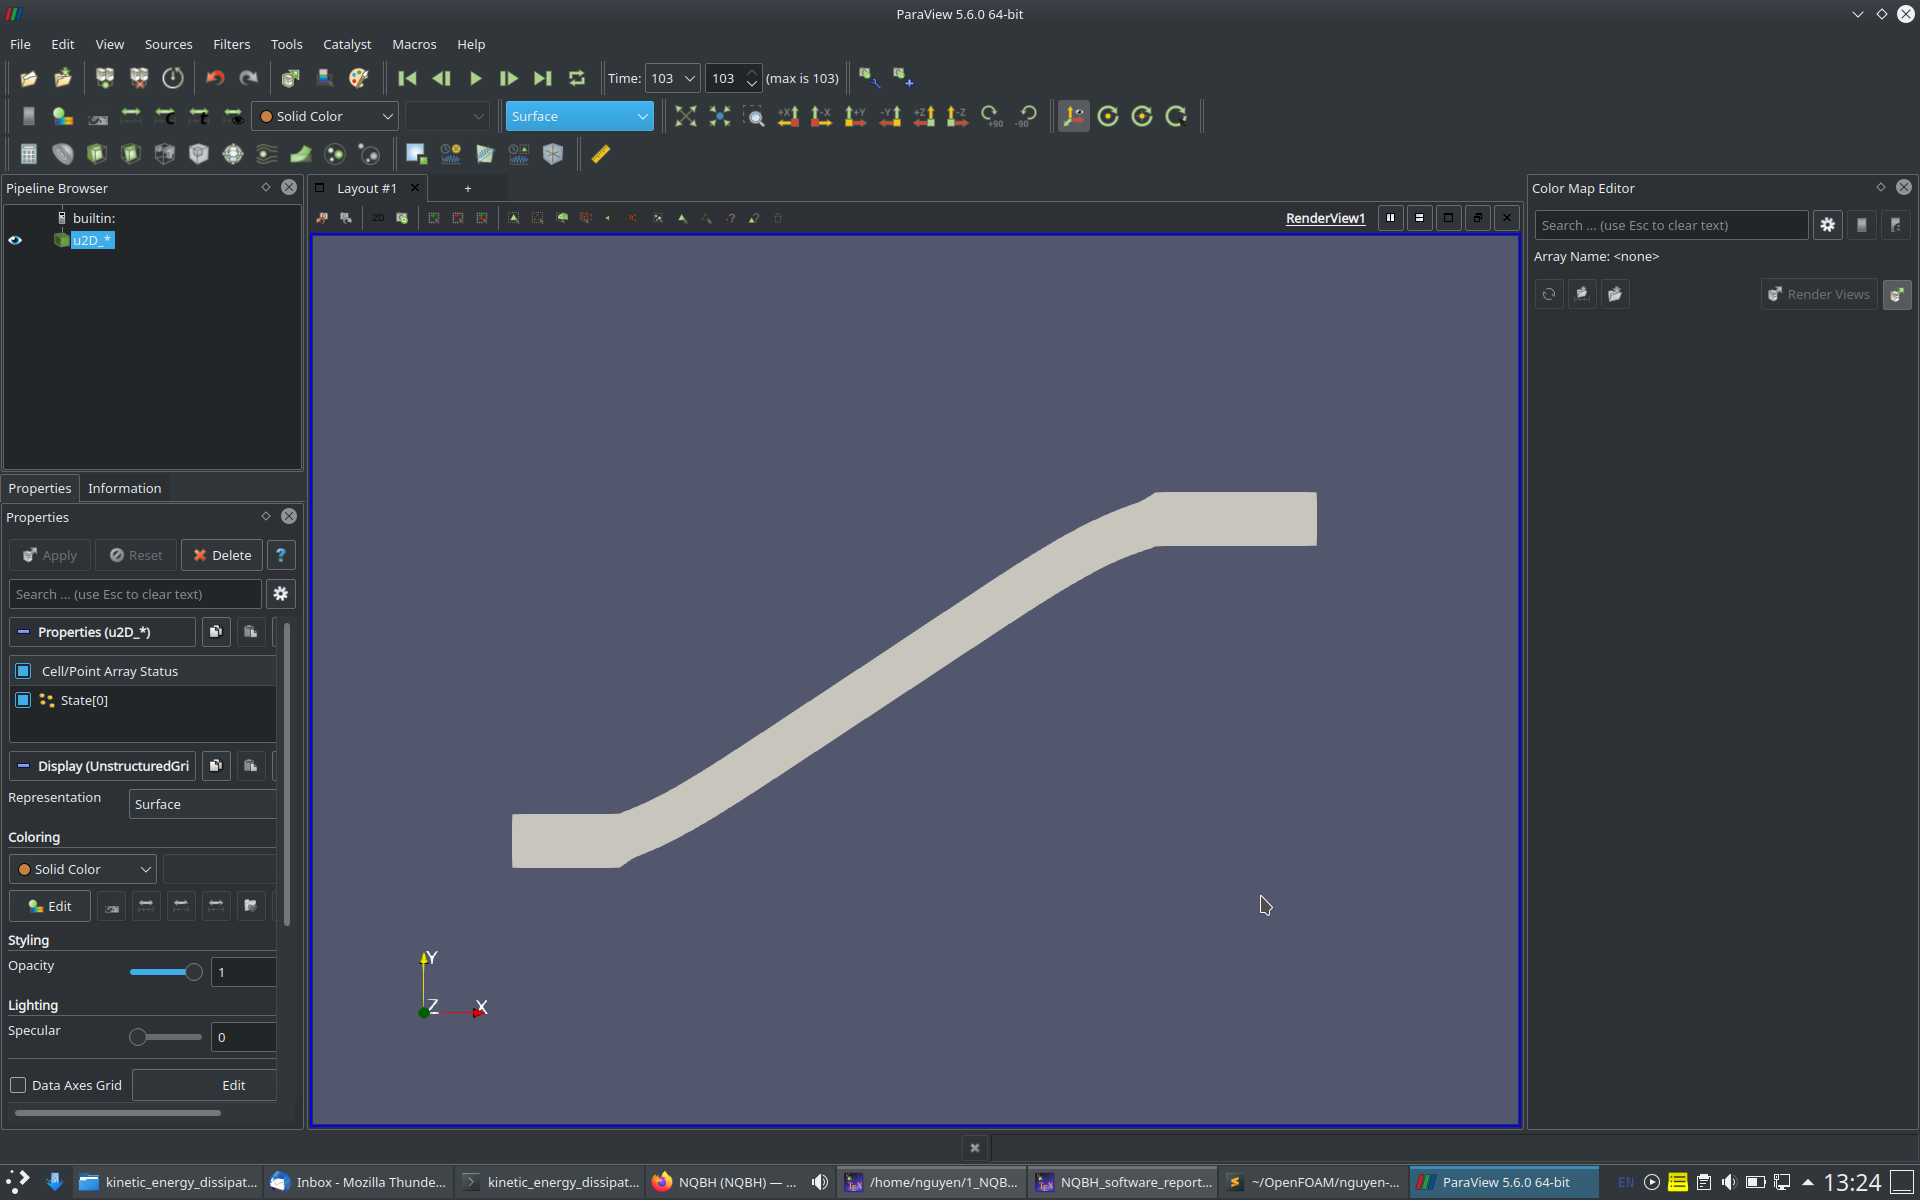
\includegraphics[height=0.44\textheight]{optimized_domain_2D_after_103_steps_Solid_Color_Surface}
            \caption{View the optimized 2D domain after 103 optimization steps by ParaView with modes: \texttt{Solid Color, Surface}.}
        \end{figure}
        
        \begin{figure}[H]
            \centering
            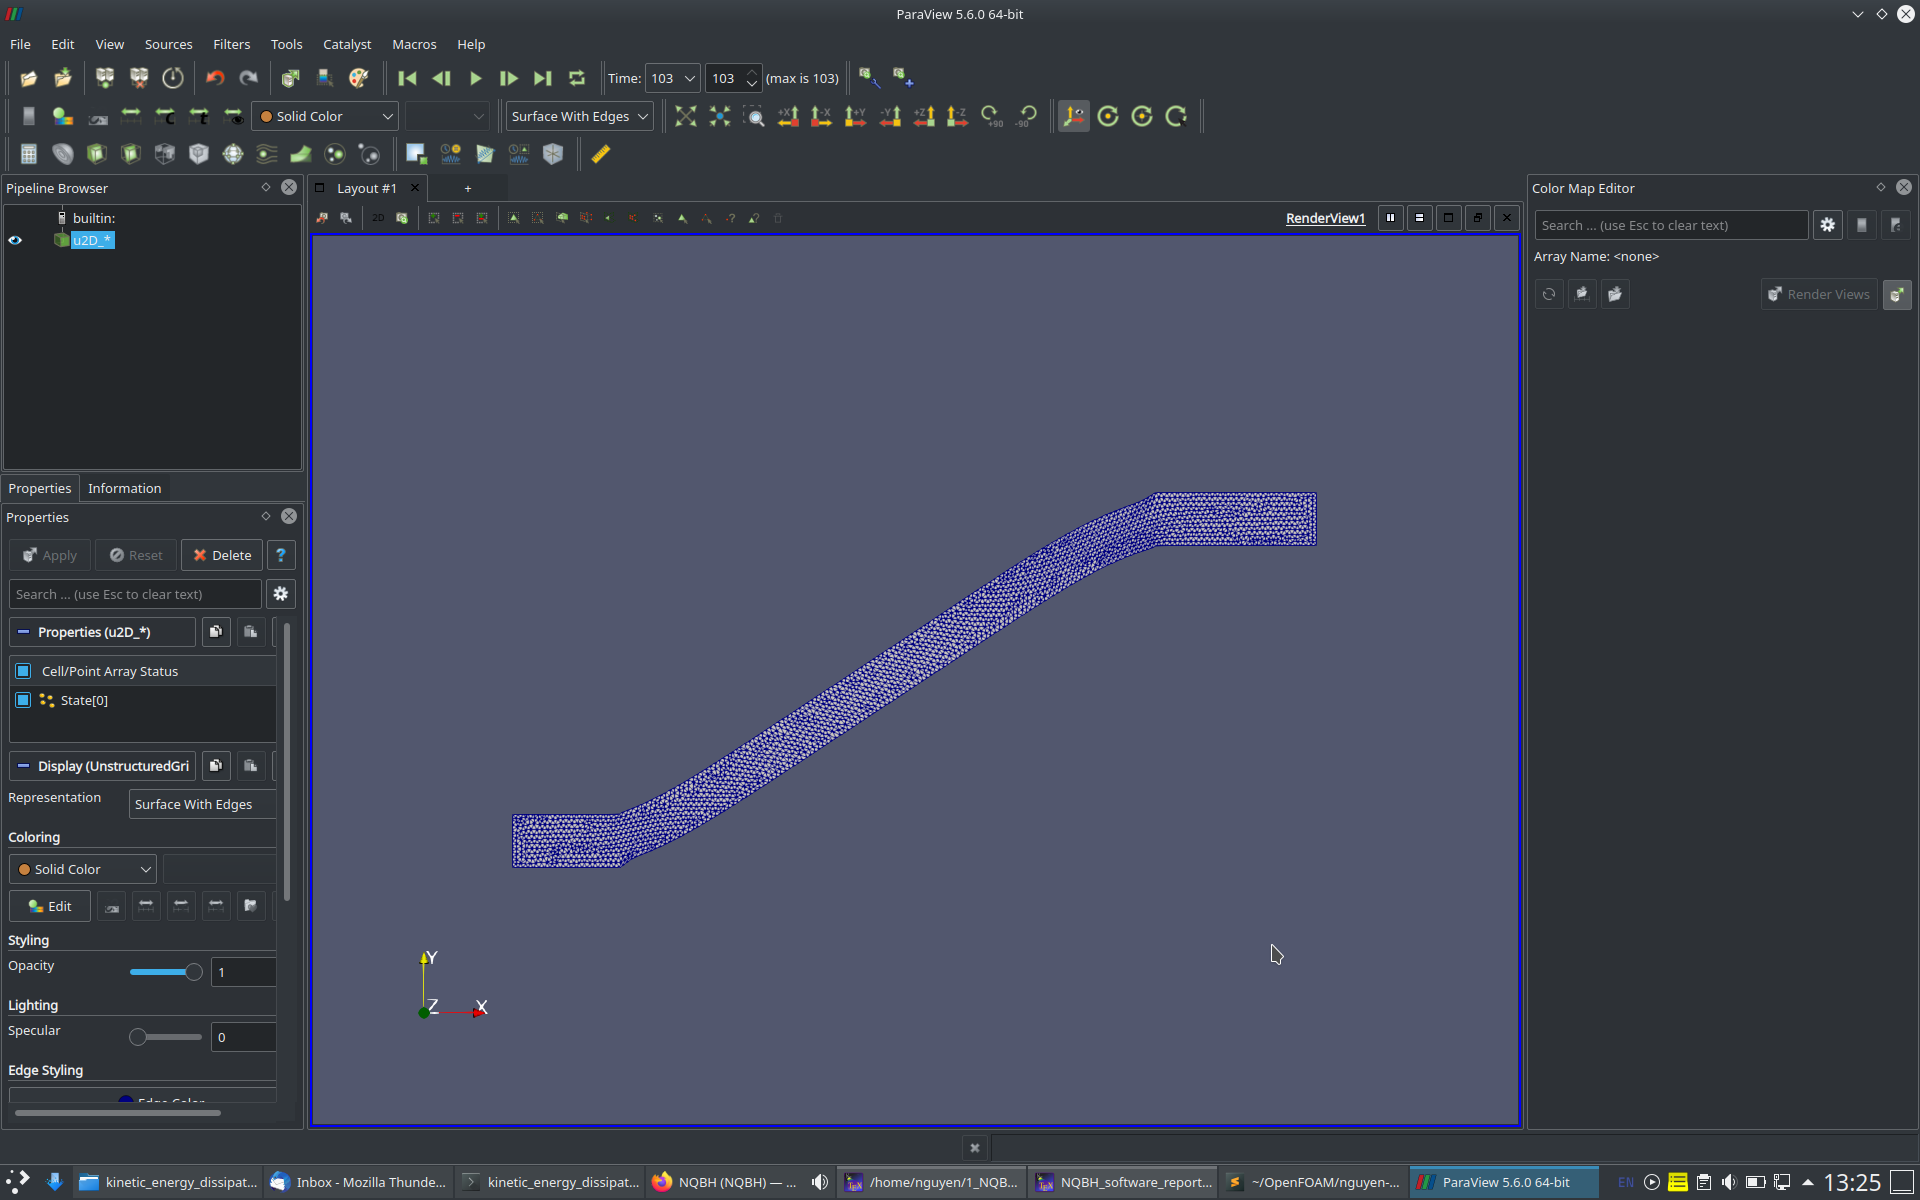
\includegraphics[height=0.44\textheight]{optimized_domain_2D_after_103_steps_Solid_Color_Surface_with_Edges}
            \caption{View the optimized 2D domain after 103 optimization steps by ParaView with modes: \texttt{Solid Color, Surface with Edges}.}
        \end{figure}
        
        %
        \begin{figure}[H]
            \centering
            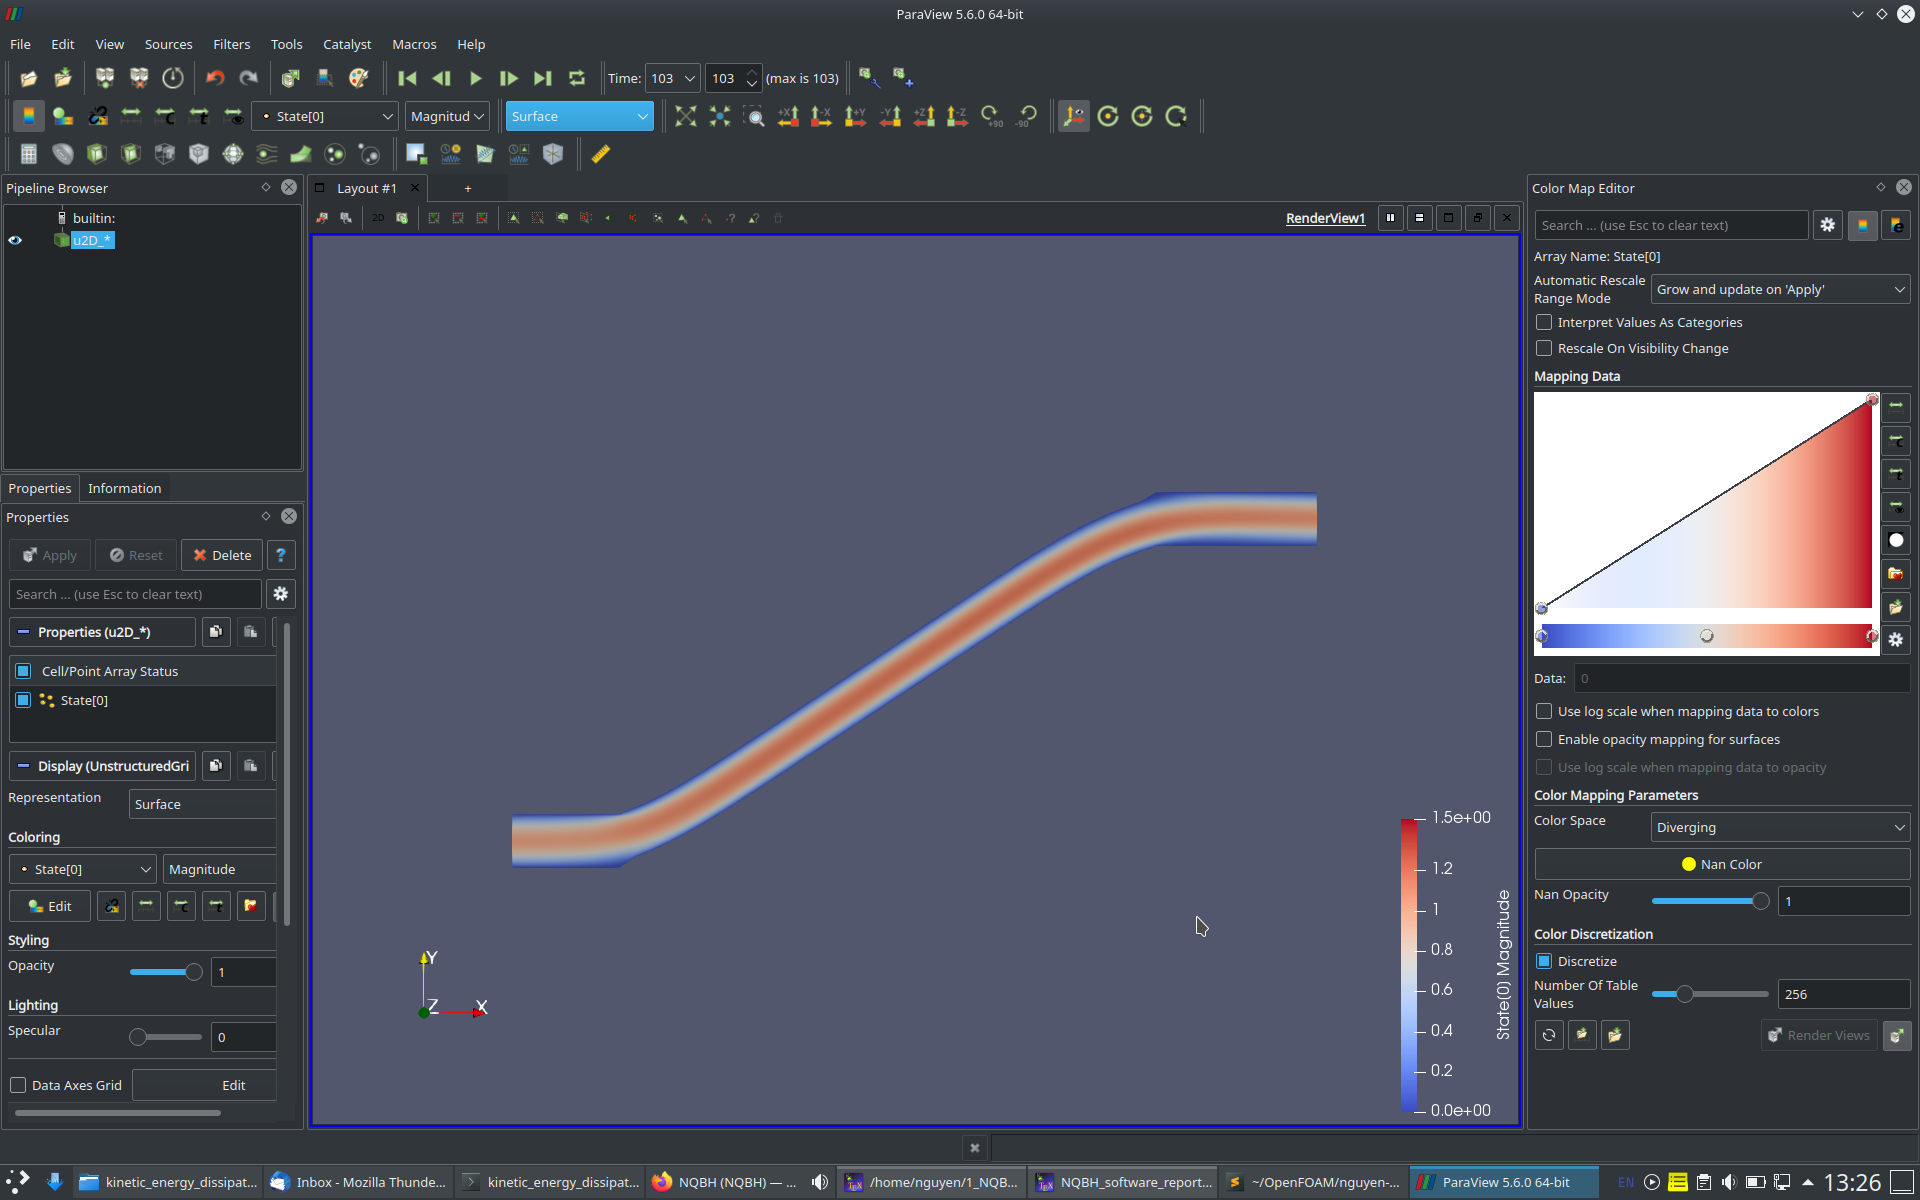
\includegraphics[height=0.44\textheight]{optimized_domain_2D_after_103_steps_State0_Surface}
            \caption{View the optimized 2D domain after 103 optimization steps by ParaView with modes: \texttt{State[0], Surface}.}
        \end{figure}
        
        \begin{figure}[H]
            \centering
            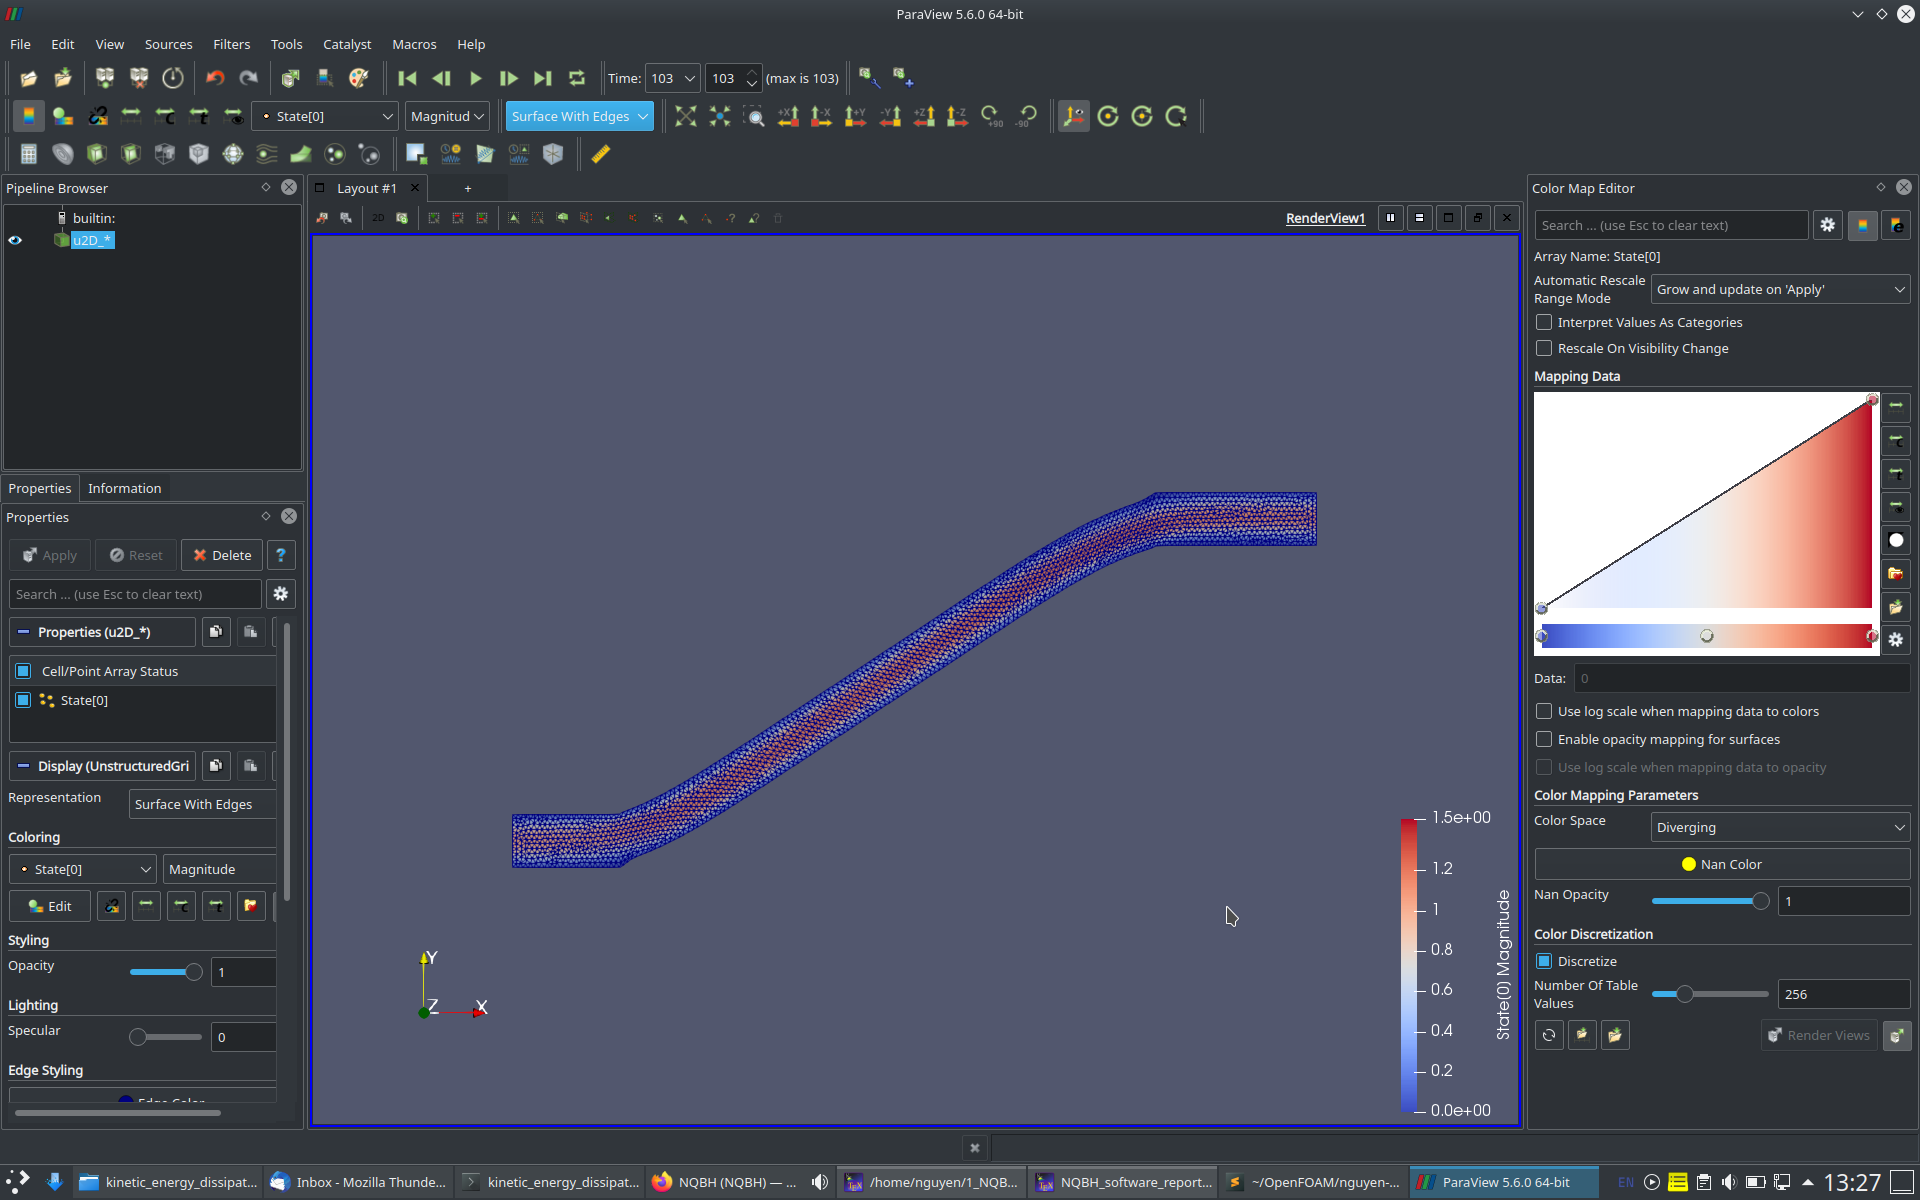
\includegraphics[height=0.44\textheight]{optimized_domain_2D_after_103_steps_State0_Surface_with_Edges}
            \caption{View the optimized 2D domain after 103 optimization steps by ParaView with modes: \texttt{State[0], Surface with Edges}.}
        \end{figure}
    
        %
        \begin{figure}[H]
            \centering
            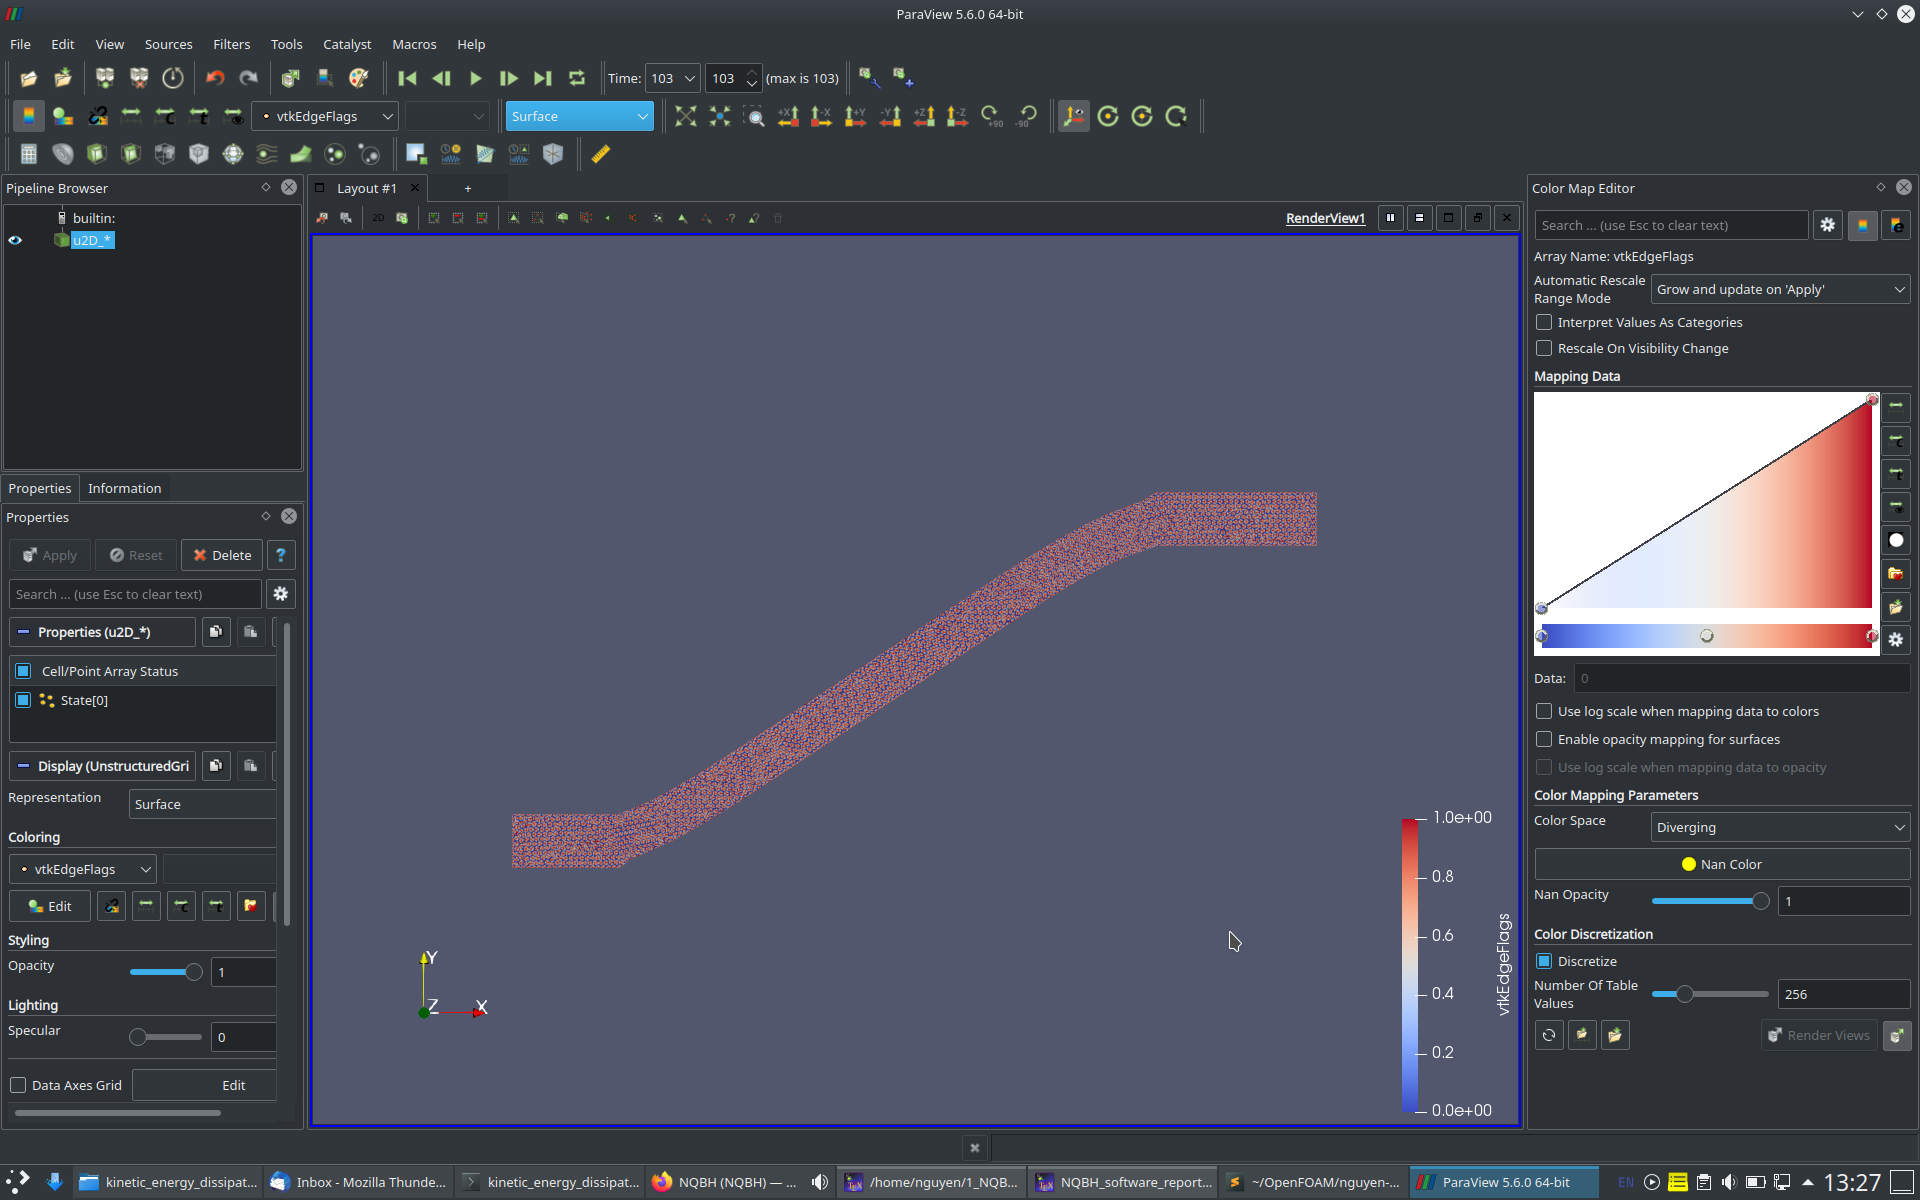
\includegraphics[height=0.44\textheight]{optimized_domain_2D_after_103_steps_vtkEdgeFlags_Surface}
            \caption{View the optimized 2D domain after 103 optimization steps by ParaView with modes: \texttt{vtkEdgeFlags, Surface}.}
        \end{figure}
        
        \begin{figure}[H]
            \centering
            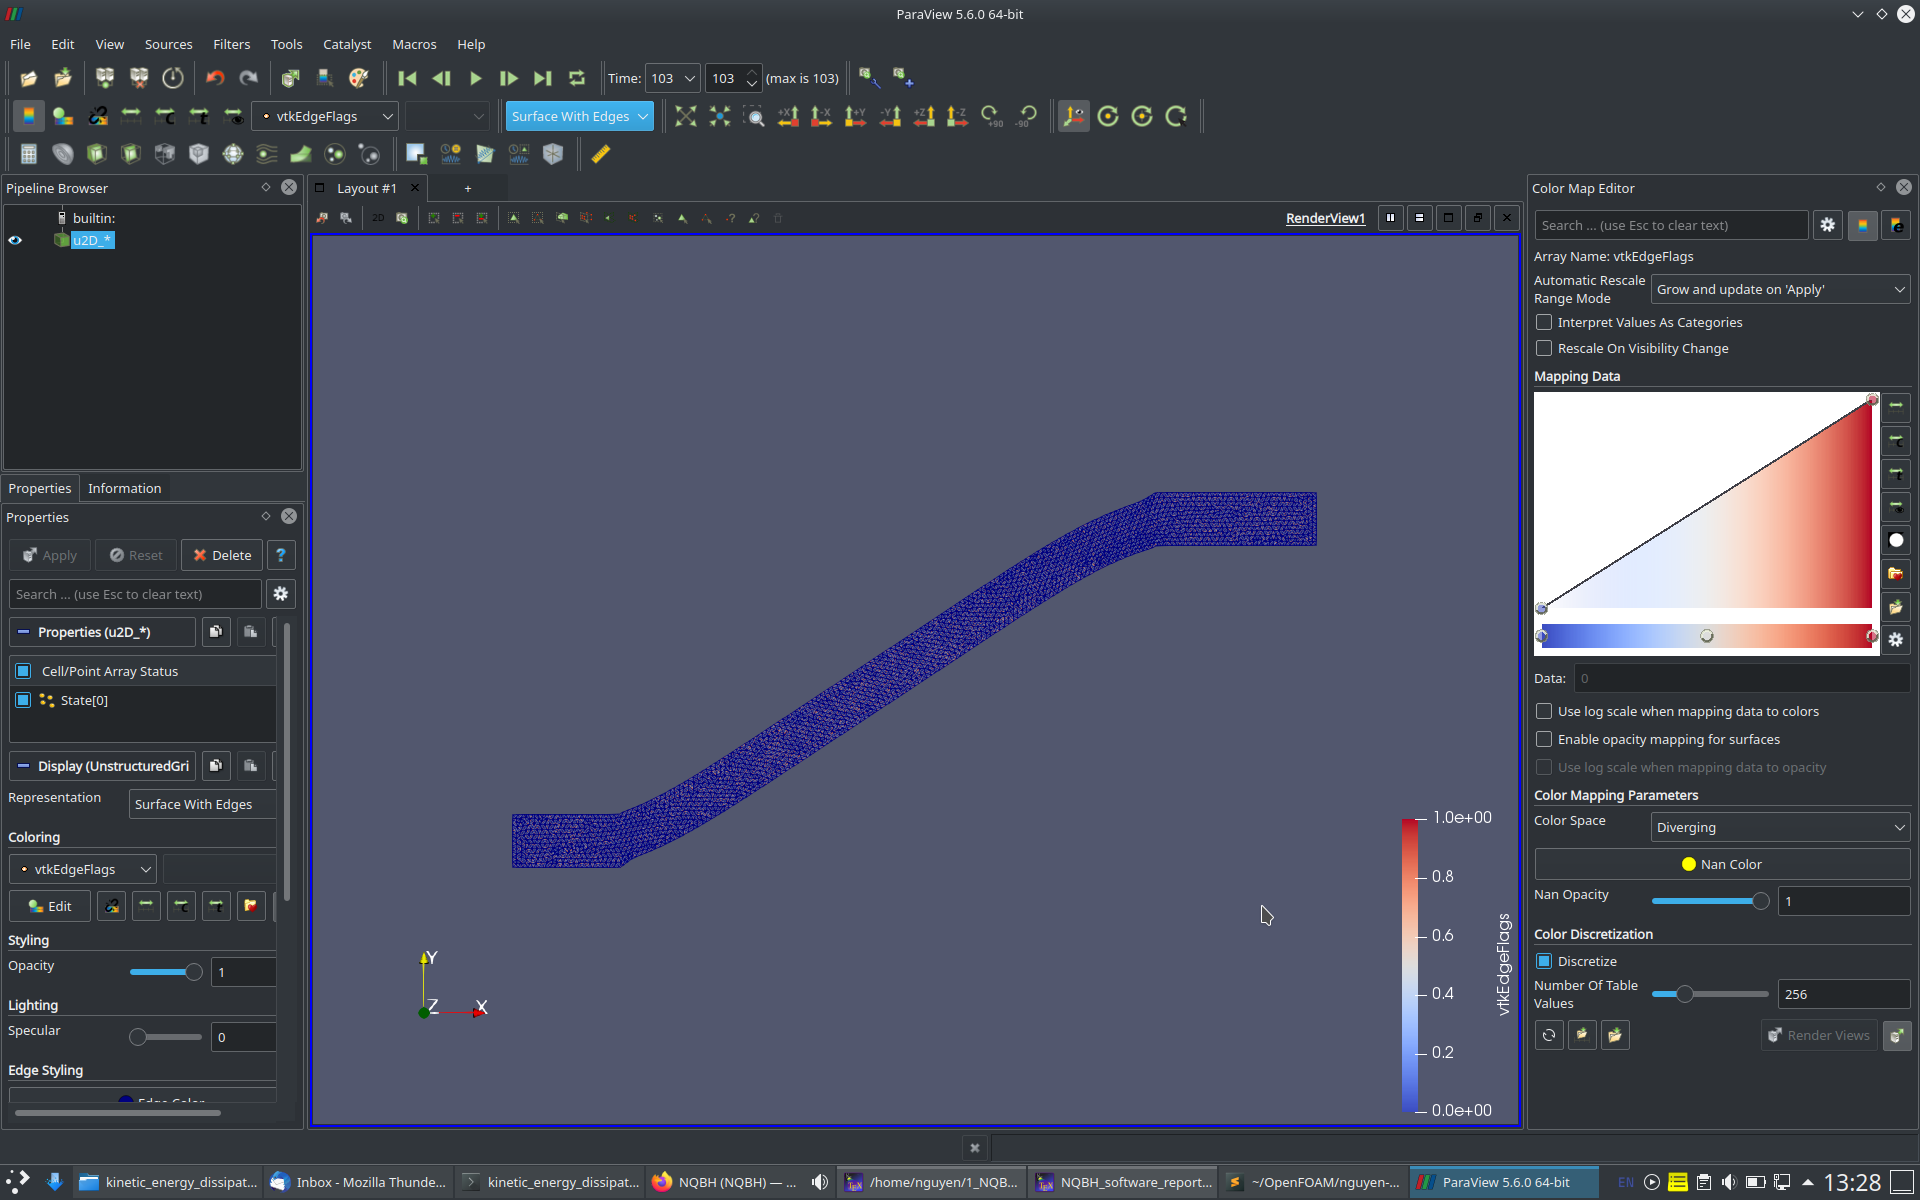
\includegraphics[height=0.44\textheight]{optimized_domain_2D_after_103_steps_vtkEdgeFlags_Surface_with_Edges}
            \caption{View the optimized 2D domain after 103 optimization steps by ParaView with modes: \texttt{vtkEdgeFlags, Surface with Edges}.}
        \end{figure}

        $\star$ \textbf{3D.}
        
        \begin{figure}[H]
            \centering
            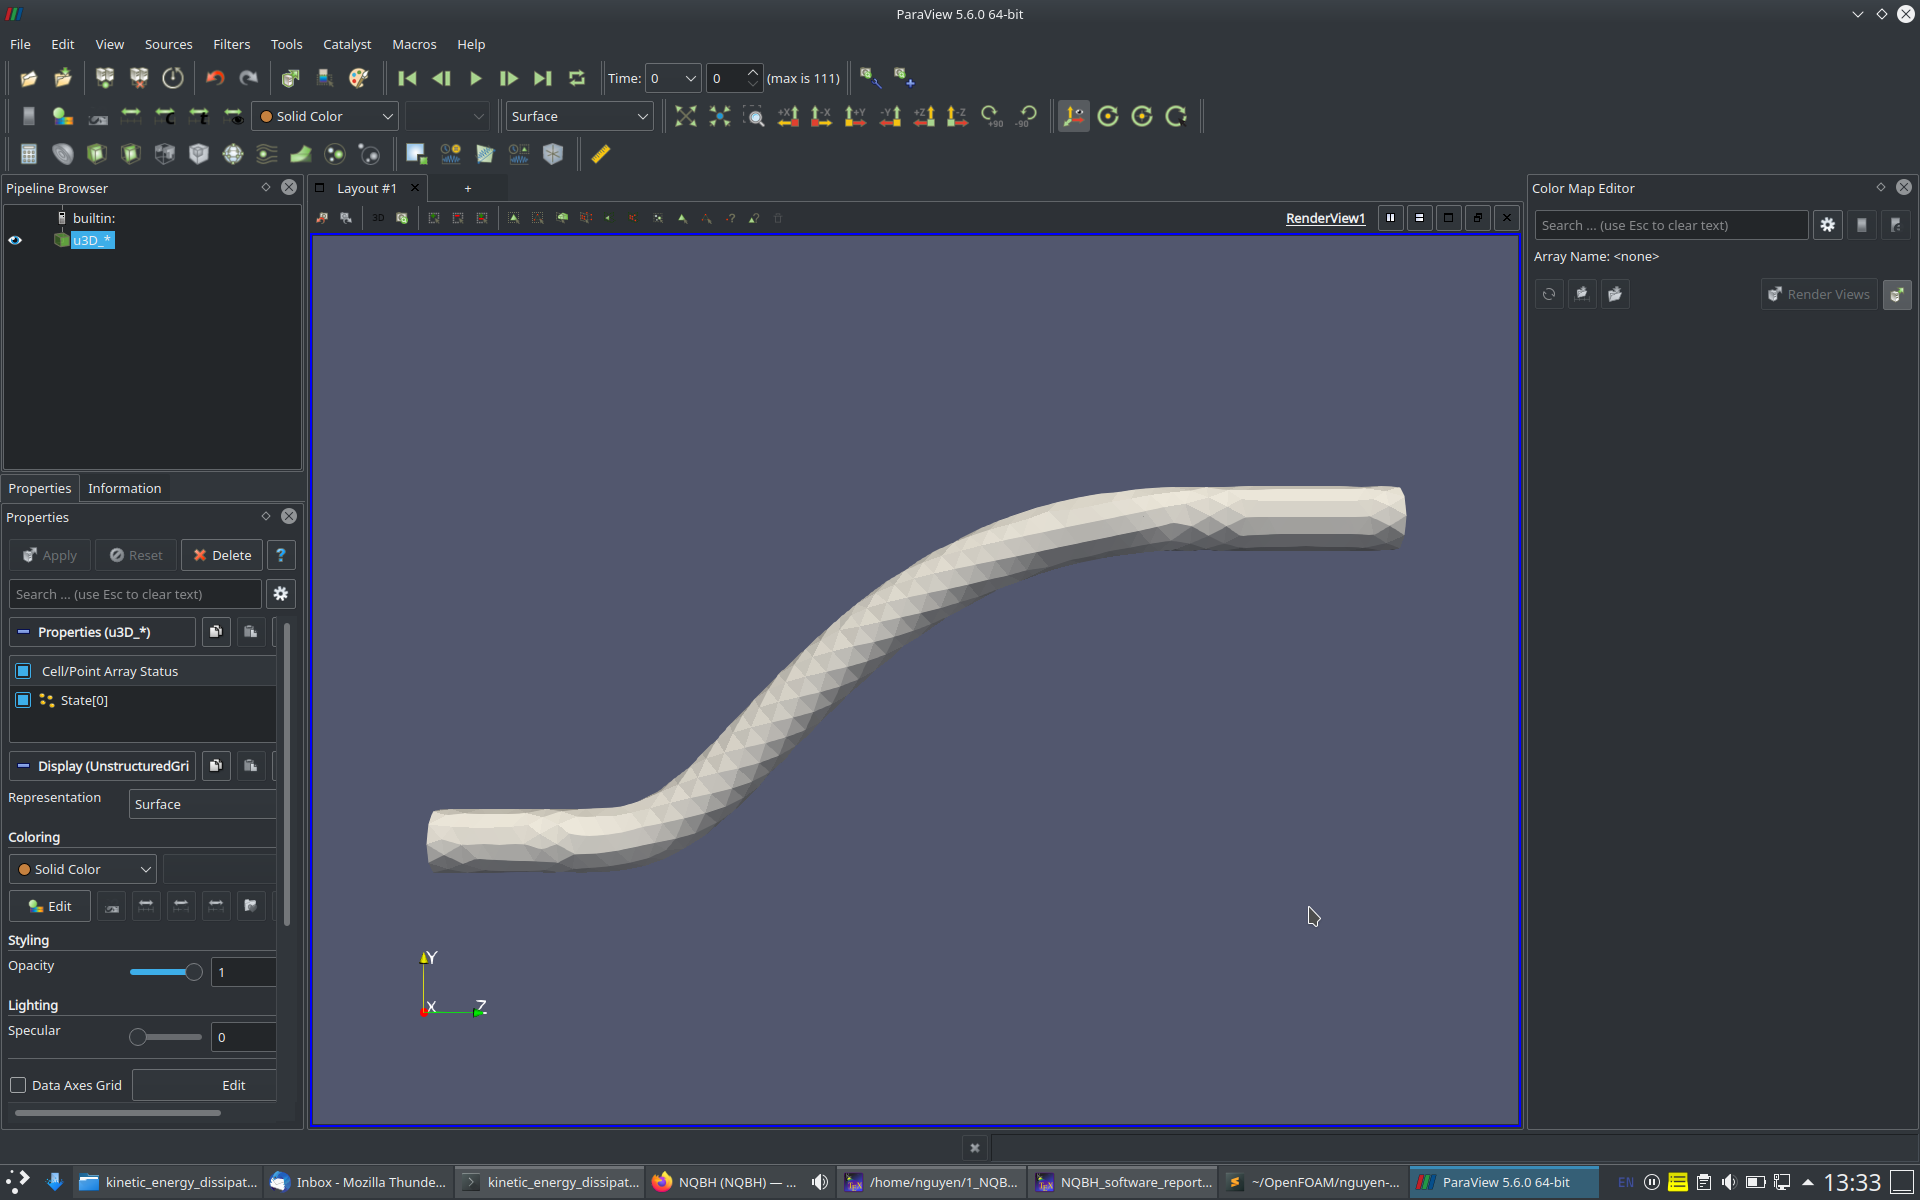
\includegraphics[height=0.44\textheight]{initial_domain_3D_Solid_Color_Surface}
            \caption{View the initial 3D domain by ParaView with modes: \texttt{Solid Color, Surface}.}
        \end{figure}
        
        \begin{figure}[H]
            \centering
            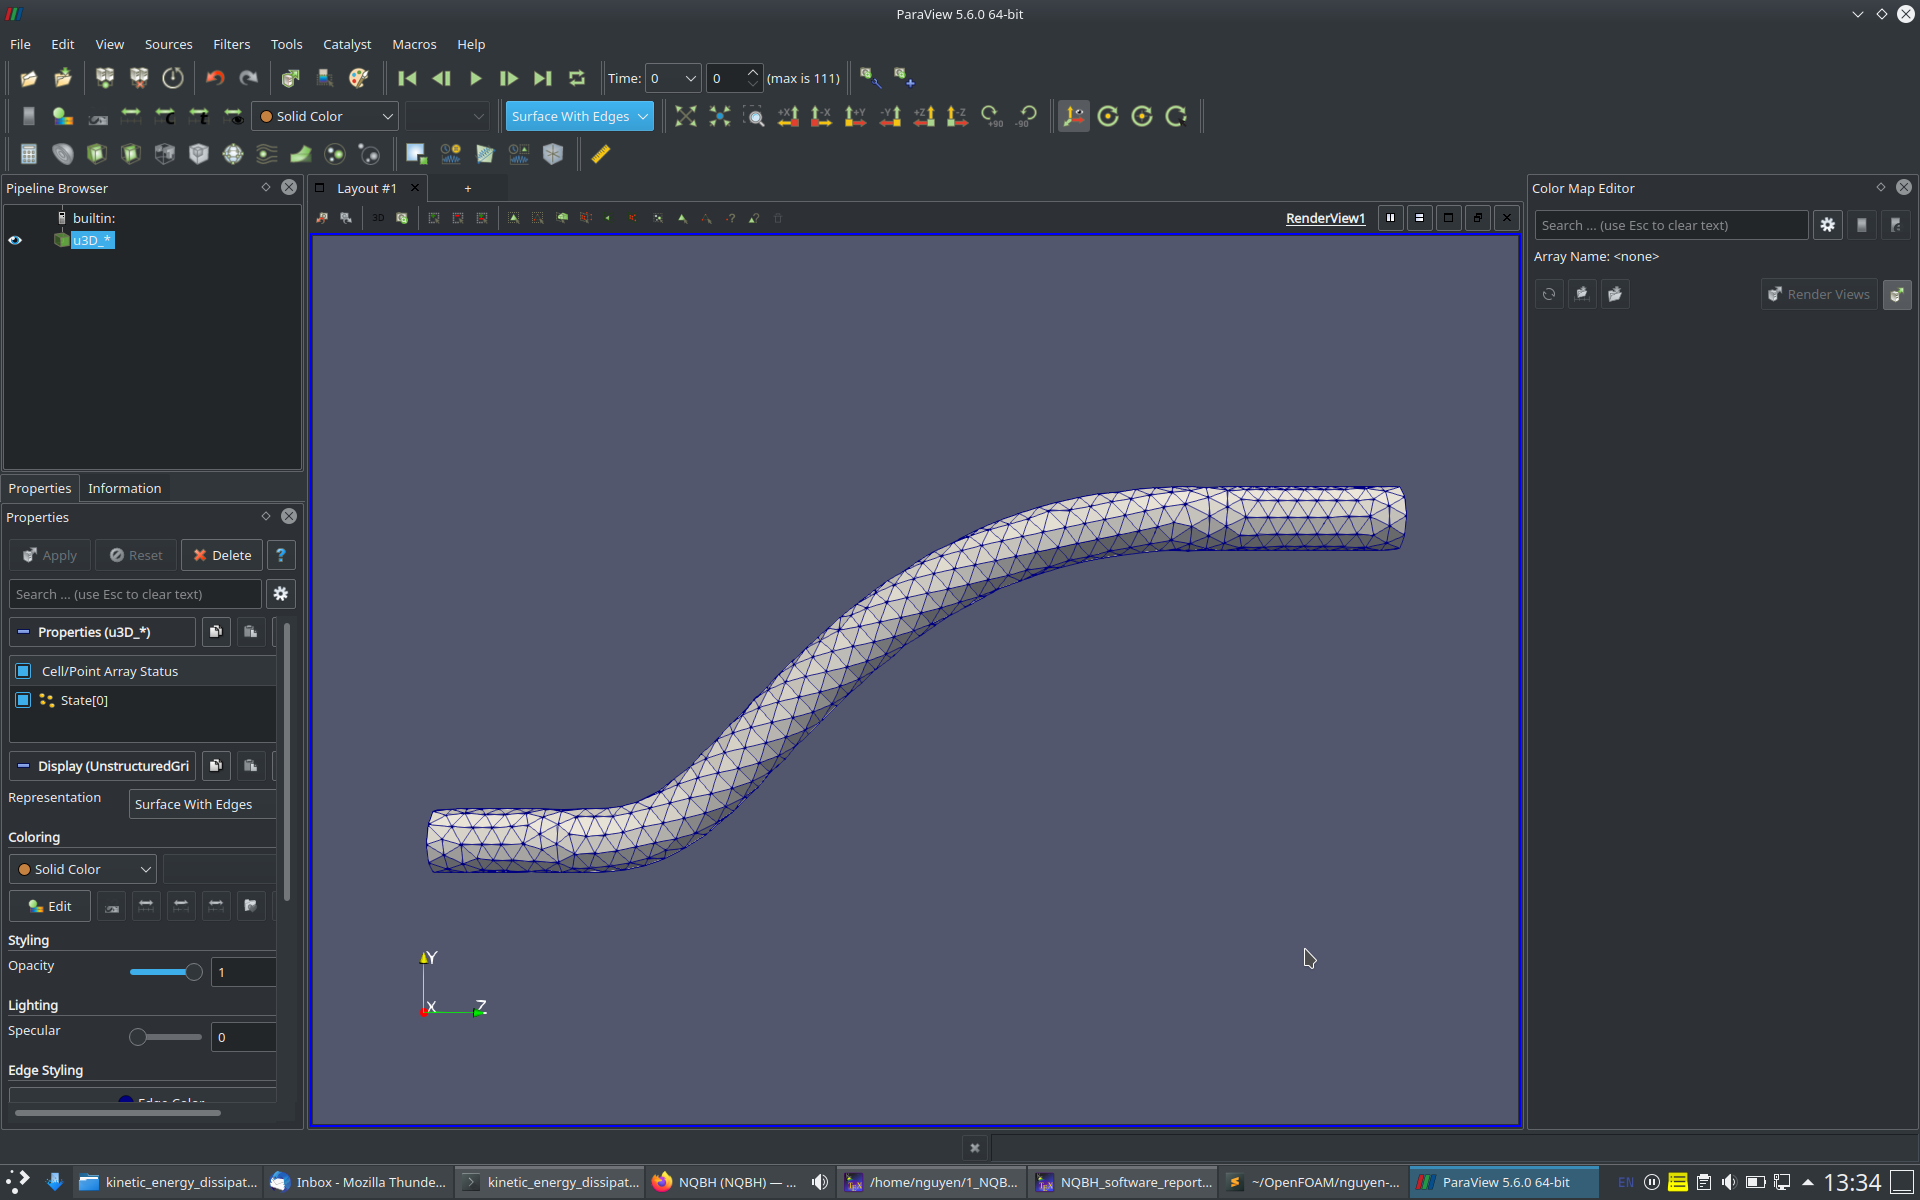
\includegraphics[height=0.44\textheight]{initial_domain_3D_Solid_Color_Surface_with_Edges}
            \caption{View the initial 3D domain by ParaView with modes: \texttt{Solid Color, Surface with Edges}.}
        \end{figure}
    
        %
        \begin{figure}[H]
            \centering
            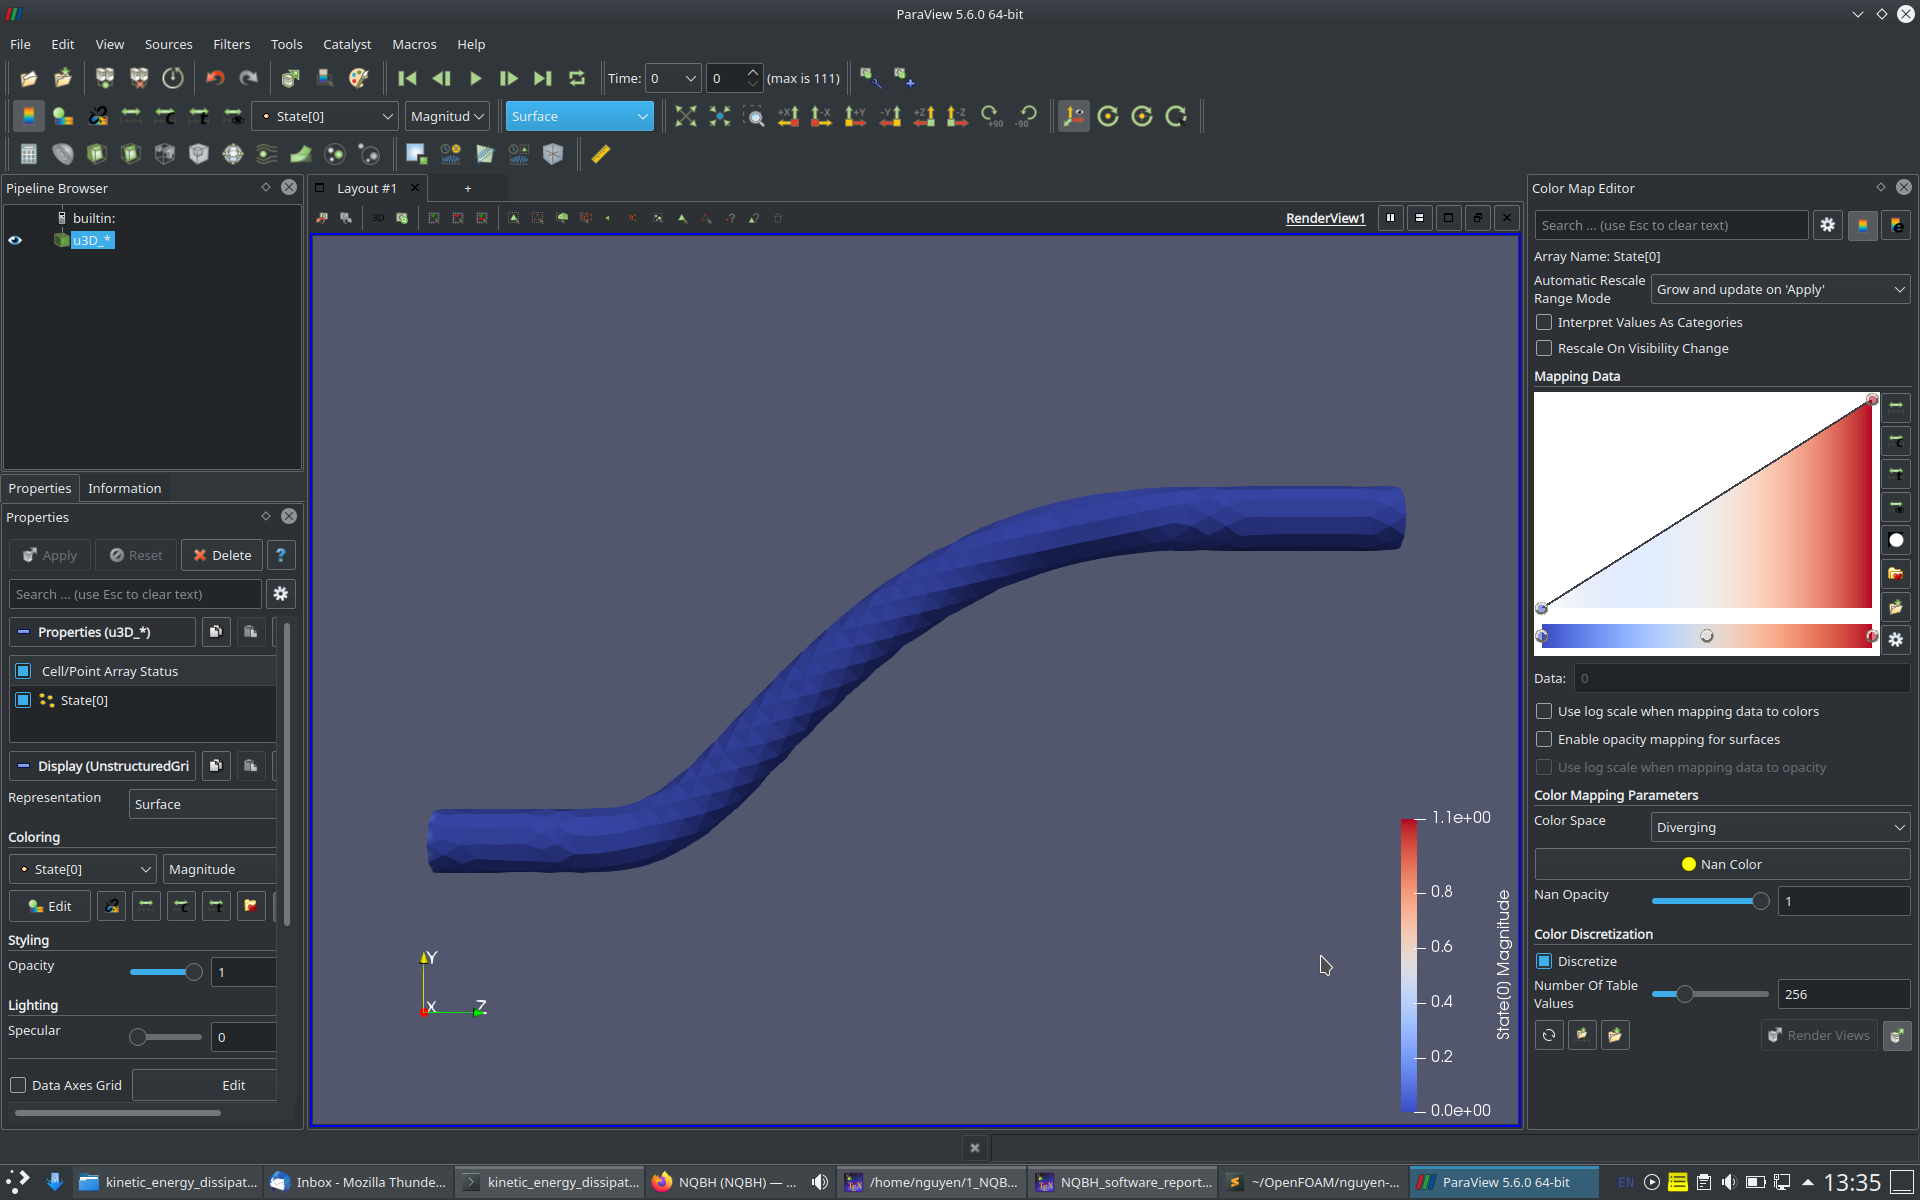
\includegraphics[height=0.44\textheight]{initial_domain_3D_State0_Surface}
            \caption{View the initial 3D domain by ParaView with modes: \texttt{State[0], Surface}.}
        \end{figure}
        
        \begin{figure}[H]
            \centering
            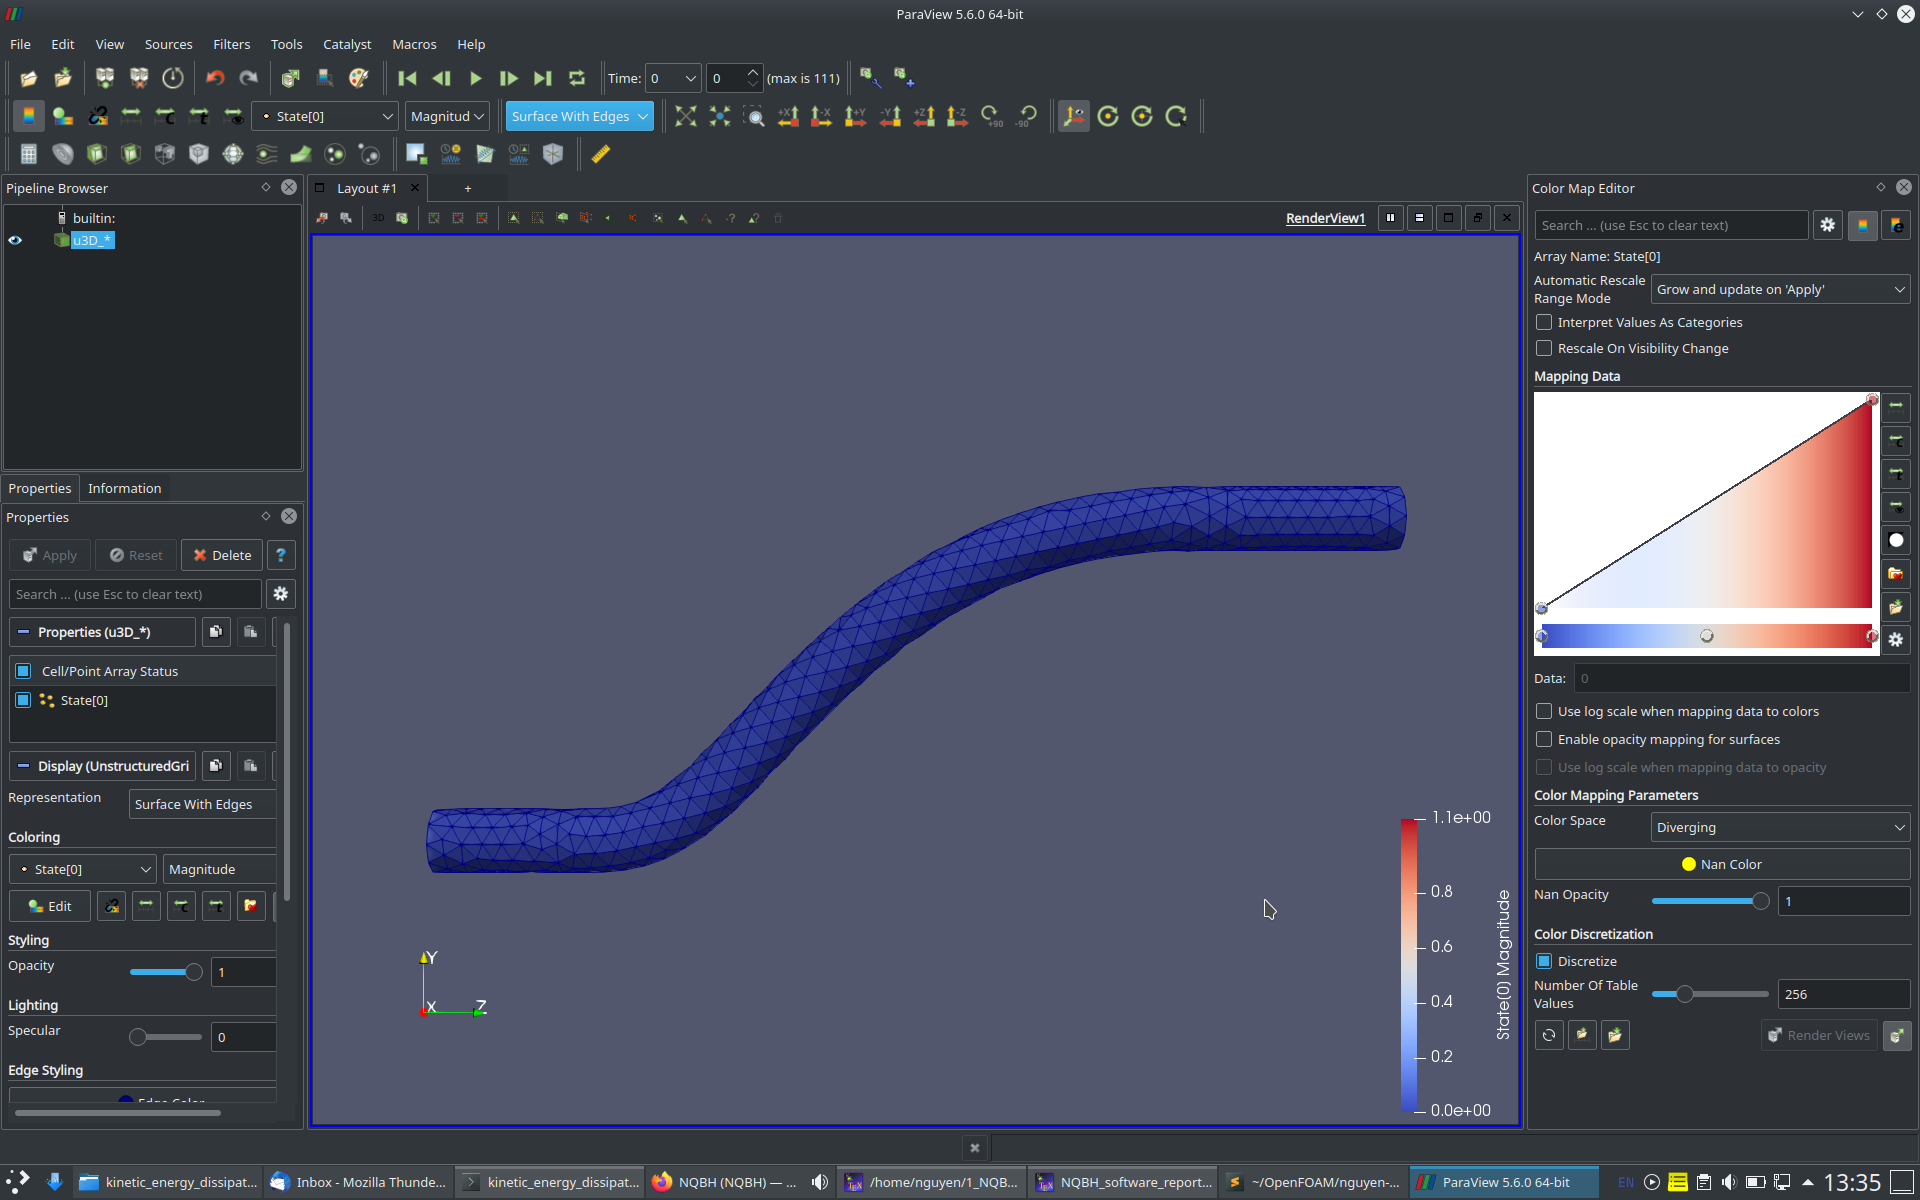
\includegraphics[height=0.44\textheight]{initial_domain_3D_State0_Surface_with_Edges}
            \caption{View the initial 3D domain by ParaView with modes: \texttt{State[0], Surface with Edges}.}
        \end{figure}
    
        %
        \begin{figure}[H]
            \centering
            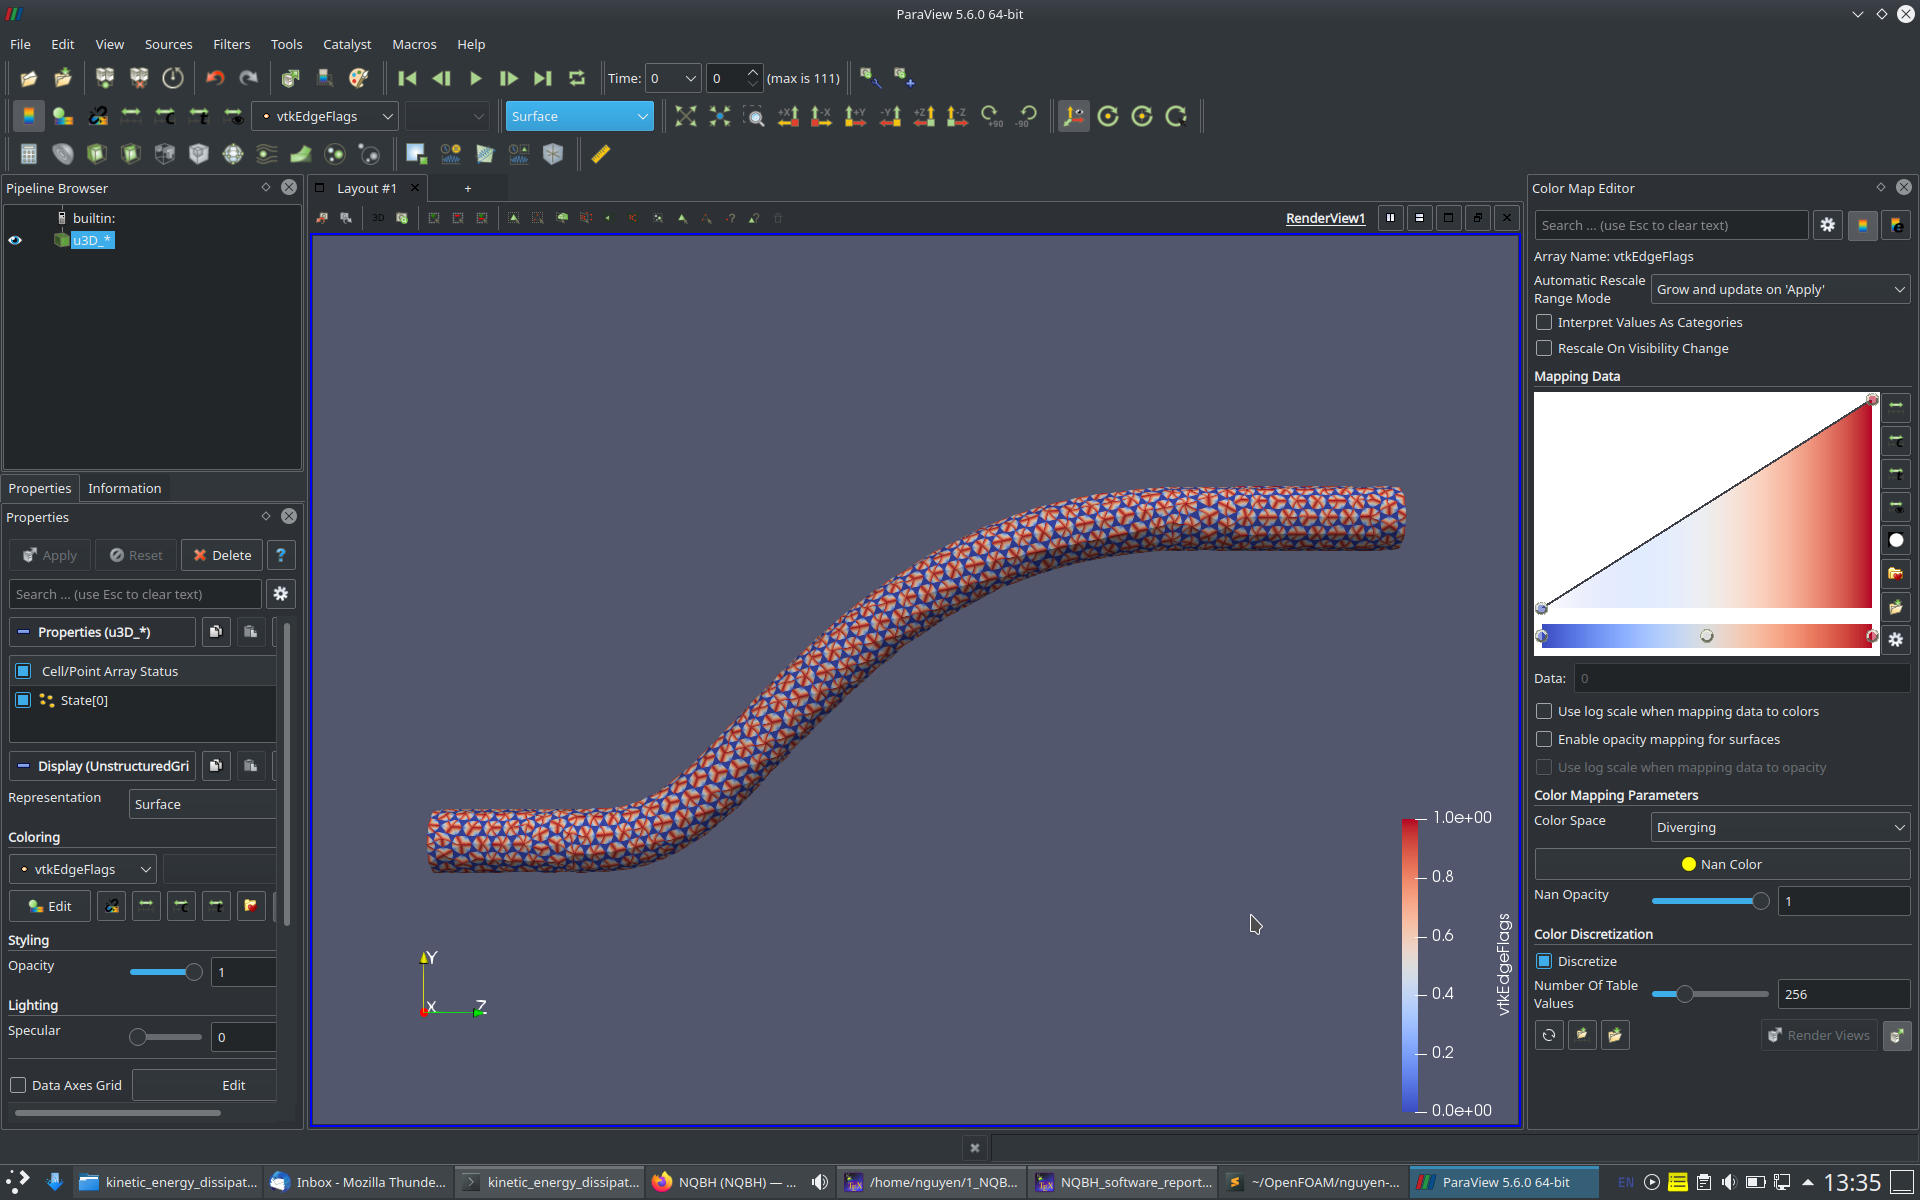
\includegraphics[height=0.44\textheight]{initial_domain_3D_vtkEdgeFlags_Surface}
            \caption{View the initial 3D domain by ParaView with modes: \texttt{vtkEdgeFlags, Surface}.}
        \end{figure}
        
        \begin{figure}[H]
            \centering
            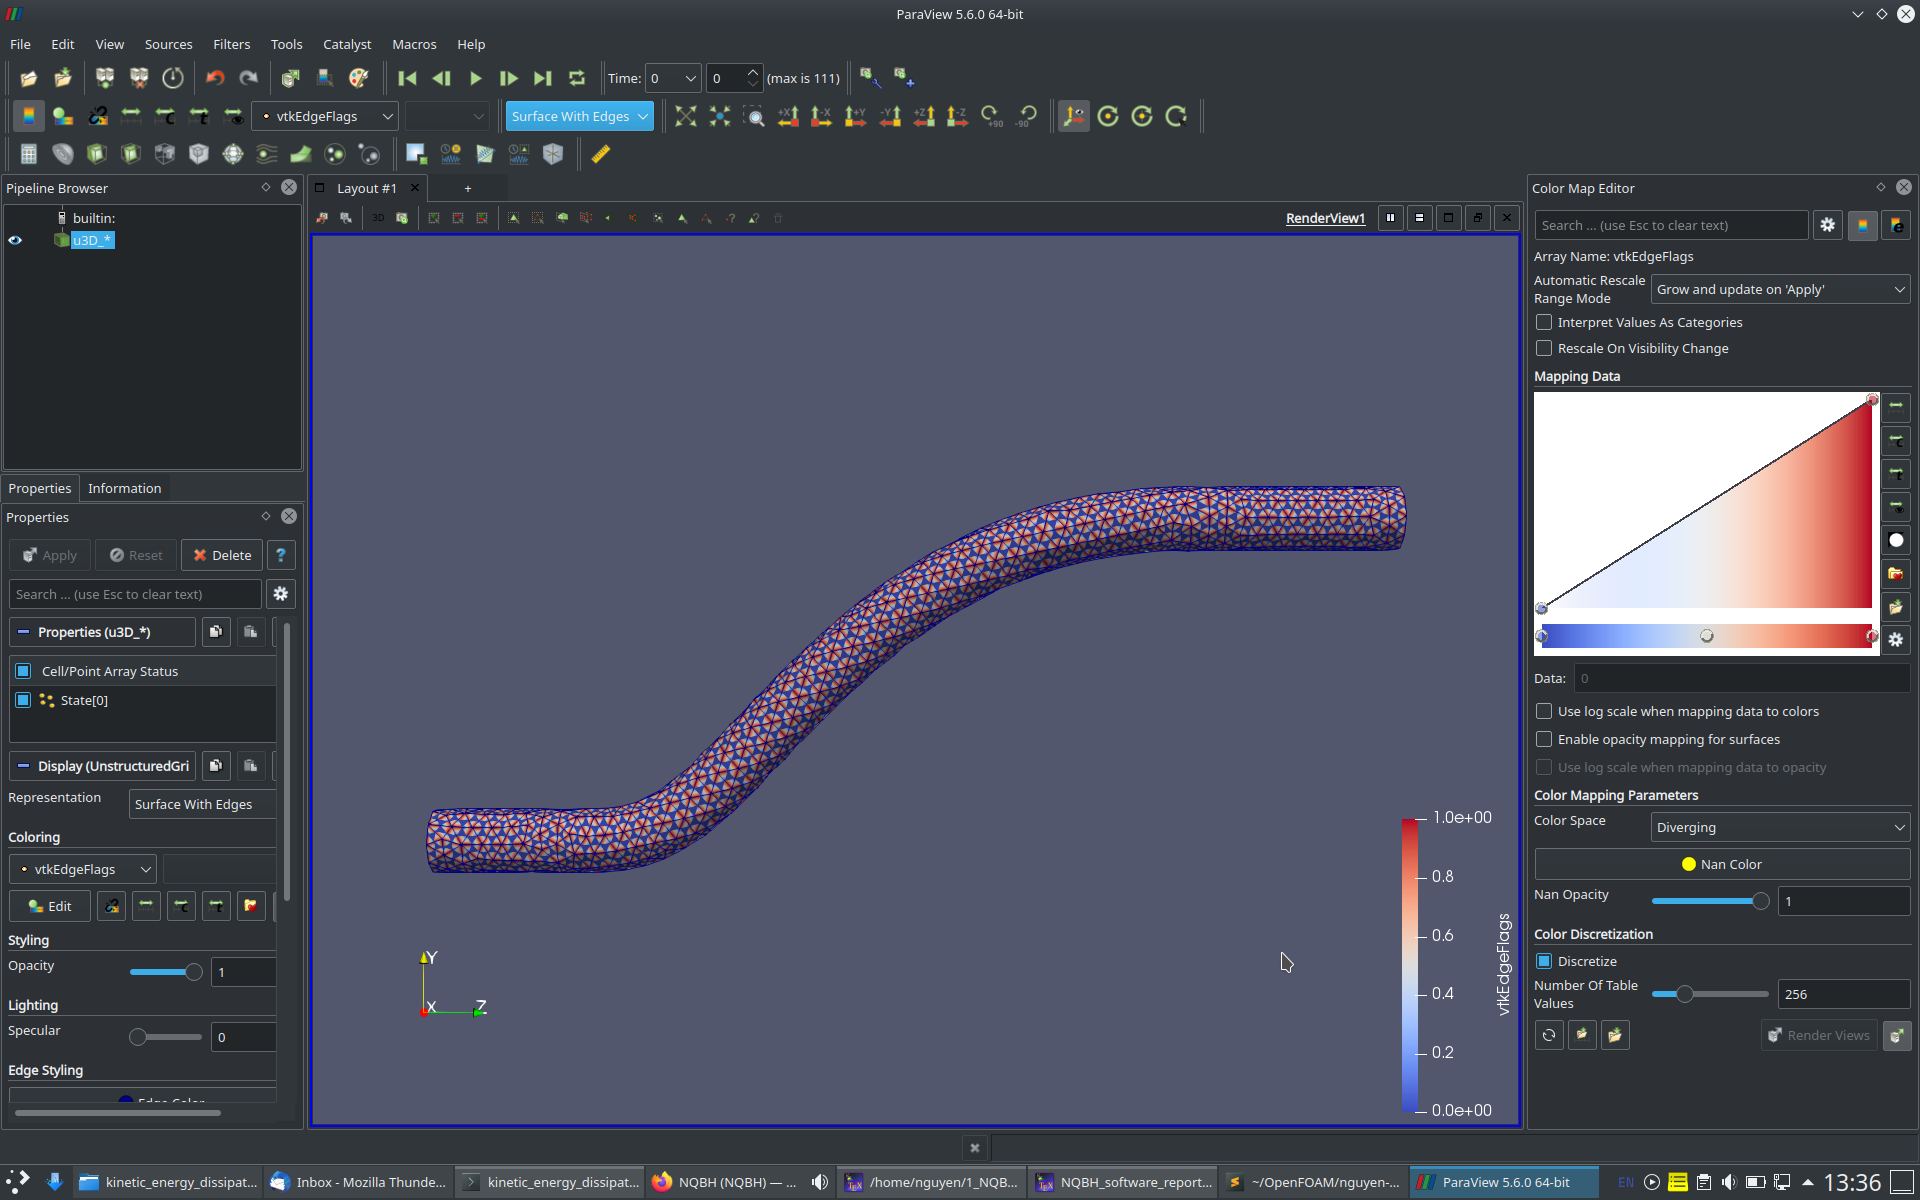
\includegraphics[height=0.44\textheight]{initial_domain_3D_vtkEdgeFlags_Surface_with_Edges}
            \caption{View the initial 3D domain by ParaView with modes: \texttt{vtkEdgeFlags, Surface with Edges}.}
        \end{figure}
    
        %        
        \begin{figure}[H]
            \centering
            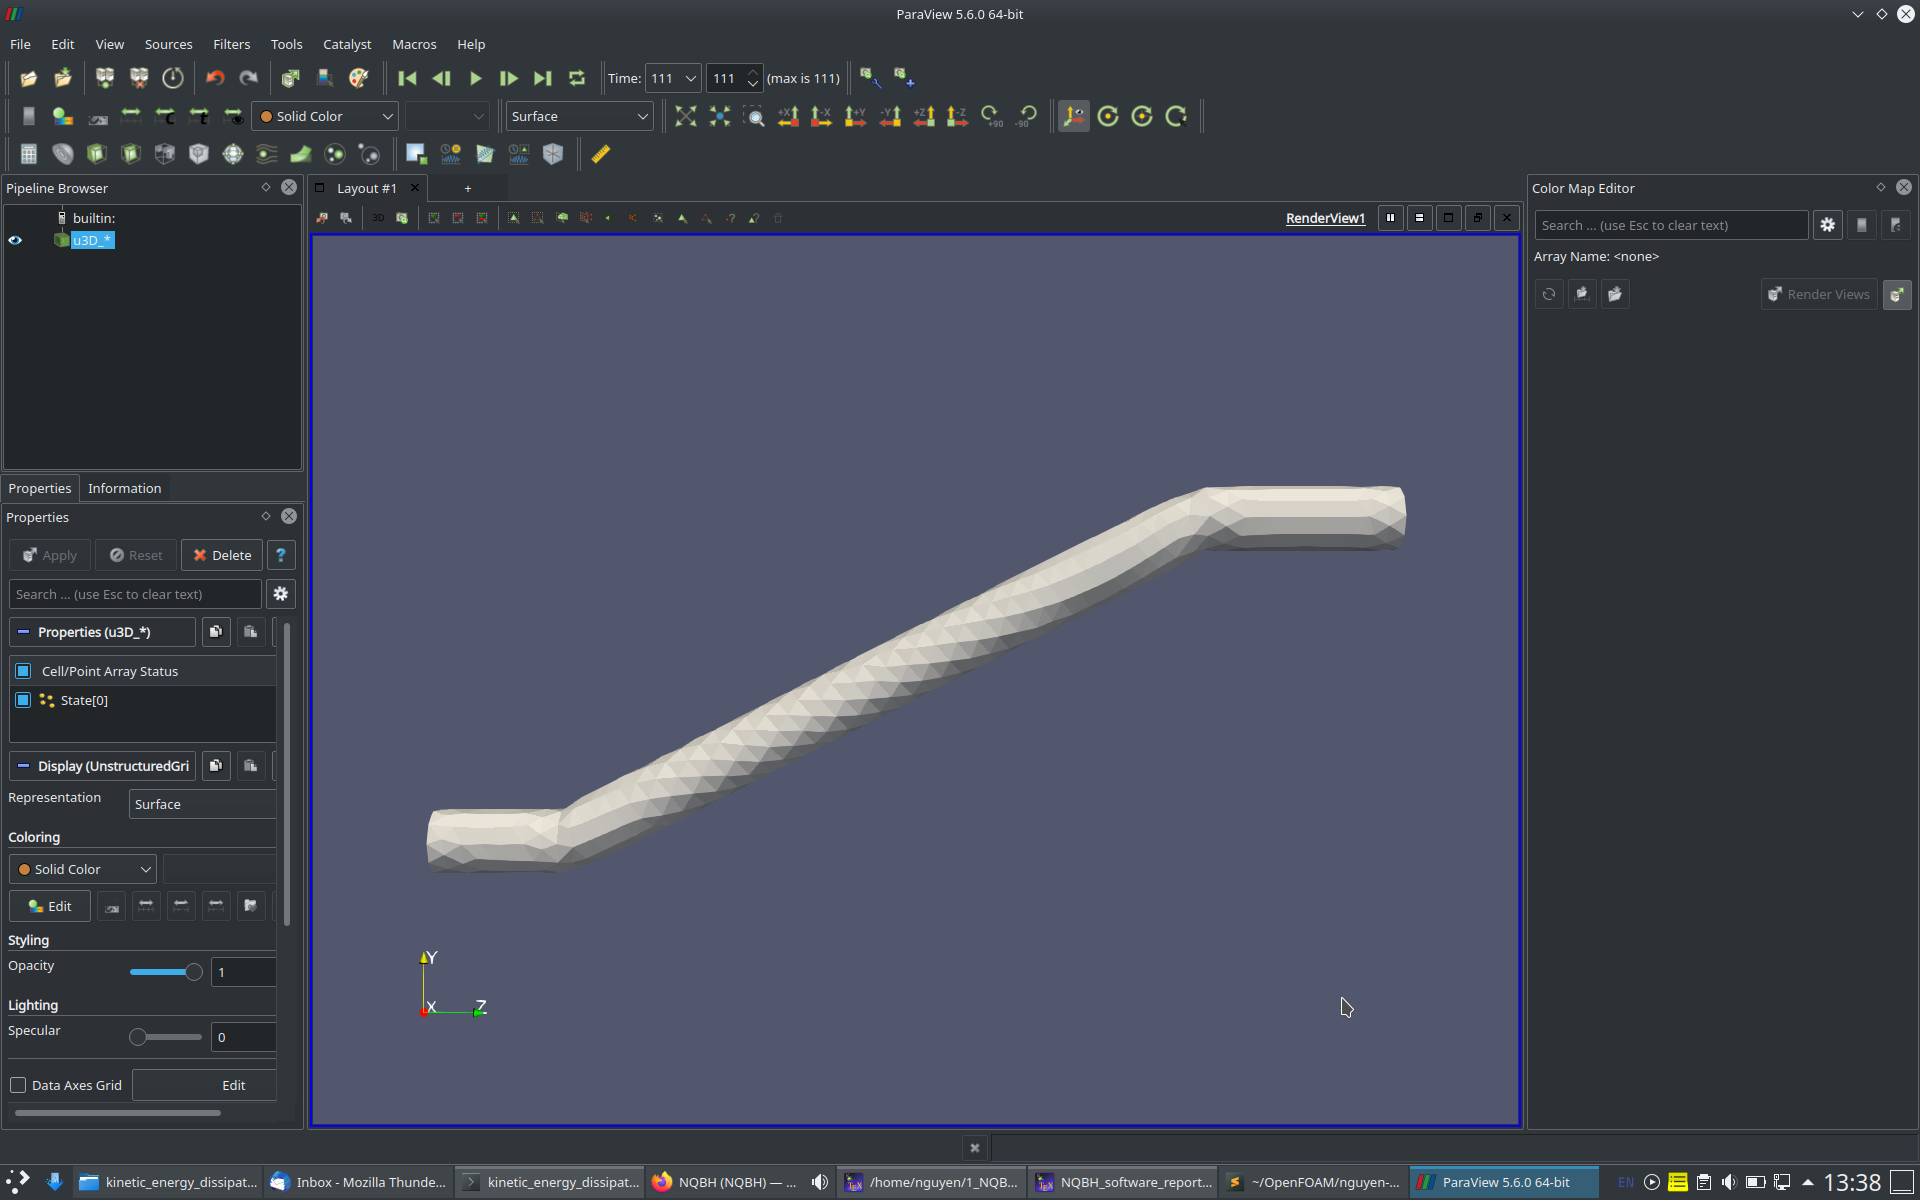
\includegraphics[height=0.44\textheight]{optimized_domain_3D_after_111_steps_Solid_Color_Surface}
            \caption{View the optimized 3D domain after 111 optimization steps by ParaView with modes: \texttt{Solid Color, Surface}.}
        \end{figure}
        
        \begin{figure}[H]
            \centering
            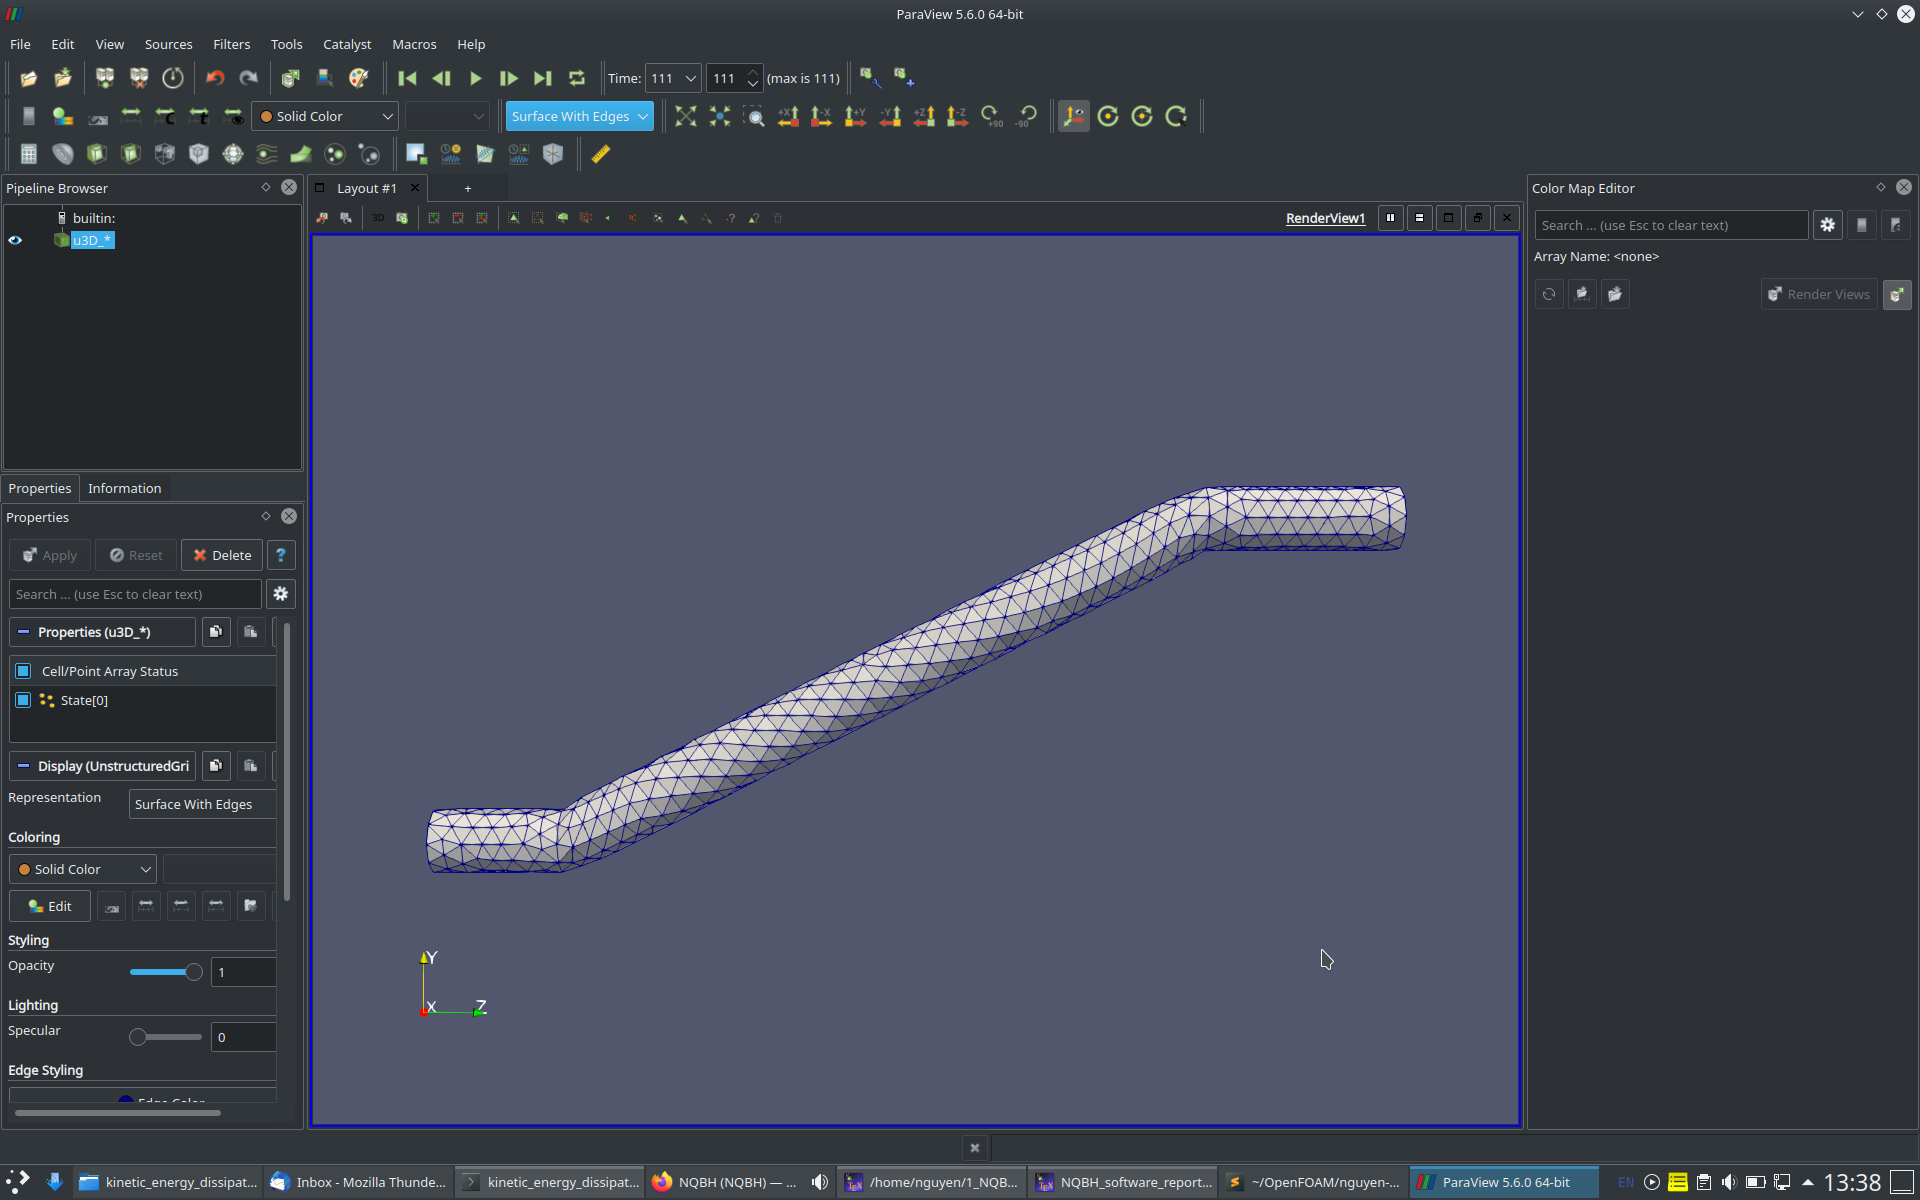
\includegraphics[height=0.44\textheight]{optimized_domain_3D_after_111_steps_Solid_Color_Surface_with_Edges}
            \caption{View the optimized 3D domain after 111 optimization steps by ParaView with modes: \texttt{Solid Color, Surface with Edges}.}
        \end{figure}
        
        %
        \begin{figure}[H]
            \centering
            \includegraphics[height=0.44\textheight]{optimized_domain_3D_after_111_steps_State0_Surface}
            \caption{View the optimized 3D domain after 111 optimization steps by ParaView with modes: \texttt{State[0], Surface}.}
        \end{figure}
        
        \begin{figure}[H]
            \centering
            \includegraphics[height=0.44\textheight]{optimized_domain_3D_after_111_steps_State0_Surface_with_Edges}
            \caption{View the optimized 3D domain after 111 optimization steps by ParaView with modes: \texttt{State[0], Surface with Edges}.}
        \end{figure}
    
        %
        \begin{figure}[H]
            \centering
            \includegraphics[height=0.44\textheight]{optimized_domain_3D_after_111_steps_vtkEdgeFlags_Surface}
            \caption{View the optimized 3D domain after 111 optimization steps by ParaView with modes: \texttt{vtkEdgeFlags, Surface}.}
        \end{figure}
        
        \begin{figure}[H]
            \centering
            \includegraphics[height=0.44\textheight]{optimized_domain_3D_after_111_steps_vtkEdgeFlags_Surface_with_Edges}
            \caption{View the optimized 3D domain after 111 optimization steps by ParaView with modes: \texttt{vtkEdgeFlags, Surface with Edges}.}
        \end{figure}
        
        \item \href{https://fireshape.readthedocs.io/en/latest/ROL.html}{\textbf{Using ROL in Fireshape}}.
        \begin{itemize}
            \item ``Fireshape allows solving shape optimization problems using the \href{https://trilinos.org/packages/rol/}{Rapid Optimization Library (ROL)}.
            \item The goal of this page is to give a very brief introduction to ROL and how to use it in Fireshape.
            \item Please note that this is not an official guide, but it's merely based on reverse engineering ROL's source code.''
        \end{itemize}
    \end{enumerate}    
\end{enumerate}

\section{SU2}
\begin{enumerate}
    \item \textbf{Website.} \url{https://su2code.github.io/}
    \item \textbf{GitHub repository.} \url{https://github.com/su2code/SU2}

    \begin{remark}
        Dr. Stephan Schmidt said that, in his opinion, SU2 is currently the best tool for multiphysics simulation and turbulence modeling.
    \end{remark}
\end{enumerate}

\section{ParMooN}
\begin{enumerate}
    \item \textbf{Website.} \url{https://cmg.cds.iisc.ac.in/parmoon/}
    \item \textbf{GitHub repository.} \url{https://github.com/sassanin/ParMooN}.
    \begin{remark}
        Prof. Volker John, Dr. Alfonso Caiazzo, and Dr. Ulrich Wilbrandt in Research Group 3, WIAS, confirmed that the version provided by this website is outdated. I contacted them and received the latest version of ParMooN already via Mercurial (hg) \url{https://repos.wias-berlin.de/ParMooN}.
    \end{remark}
    \item \textbf{References.} \cite{ParMooN2017}.
\end{enumerate}

\section{\texttt{SOFTube}}
\begin{enumerate}
    \item \textbf{Author.} Martin Kanitsar \texttt{martin.kanitsar@drei.at}
    \item \textbf{Documentation.} M. Hinterm\"uller, K. Knall, M. Kanitsar. \textit{Handbuck zur Software ``Form- un Topologieoptimierung''}. 2016 [in German only].
    
    $\to$ I have translated the Handbook to English.
    \item \textbf{Version.} Software-Version: 1612 (Dec, 2016).
    
    \begin{remark}[Outdated]
        Only compatible with OpenFOAM 2.1.1 (release date: May 31, 2012). Cannot run on the latest version \texttt{openfoam-dev} (updated \textit{weekly} to the cutting-edge developments) of OpenFOAM.
    \end{remark}    
    \item \textbf{Components}. \texttt{SOFTube} is a group of OpenFOAM-based applications, which can be divided mainly into the following 3 subgroups:
    \begin{itemize}
        \item \texttt{setupShapeGradientCCM}: usage: copy the default initial geometry from the folder \verb|$FOAM_RUN/tutorials/InitialSGccm| to the current OpenFOAM case, set up the correct the folder structure for that case, and then read parameters from \verb|parameter_sg| and then export to \verb|$FOAM_RUN/<case directory>/system/fvSolution|
        
        \begin{remark}
            In my opinion, without considering \textsc{Star-CCM+}, this step is redundant. OpenFOAM forces the users to set up the folder structure themselves and to change freely parameters in the dictionary \texttt{fvSolution} directly. Hence, if I develop my own OpenFOAM-based software, I will definitely skip this step to simplify the software elegantly and properly.
        \end{remark}
        \item \textbf{Topology Optimization subgroup.}
        \begin{itemize}
            \item \textit{Main executable OpenFOAM-based application}: \texttt{topoOpt}.
            \item \textit{Dependencies}: \texttt{cutSTL, generateFieldsFoam, splitSTLFoam, topoExtractSTL, topoOptCloseAll}.
            \item \textit{Usage}: For topology optimization, the largest possible initial geometry is considered, e.g., a sphere containing specified inlet(s) and outlet(s). Then \texttt{topoOpt} will optimize the shape by controlling porosity, i.e., removing counterproductive cells (see e.g., \cite{Othmer_Villiers_Weller2007,Othmer2008}), to obtain an acceptable initial geometry for shape optimization in the next stage.
            
            \begin{remark}
                I have not upgraded, and unintended to at the moment, \texttt{topoOpt} due to several doubts/concerns listed in Chap. 2.
            \end{remark}
        \end{itemize}  
        \item \textbf{Shape Optimization subgroup.}
        \begin{itemize}
            \item \textit{Main executable OpenFOAM-based application}: \texttt{shapeGradientCCM}
            \item \textit{Dependencies}: \texttt{shapeGradientAddSTL, shapeGradientCloseAll, shapeGradientWall}.
            \item Usage: Run in terminal (my favorite style)
            \begin{verbatim}
nguyen@escher-01:~/OpenFOAM/nguyen-v2006/run/Test-final> shapeGradientCCM 2>&1 | tee output
            \end{verbatim}
            for both the terminal output and a \texttt{output} file saving it (convenient to inspect later).
        \end{itemize}
    
        \begin{remark}
            I have upgraded Shape Optimization subgroup, with a lot of cleaning unused variables/headers and adjusting programming styles, to the latest version of OpenFOAM: \texttt{OpenFOAM-v2006}, which produces ``similar'' results to the old version \texttt{OpenFOAM-2.1.1}. ``Similar'' here is due to 1 of, or both, the following reasons:
            \begin{itemize}
                \item The new version of OpenFOAM computes more accurately than the old one (8-year difference).
                \item I upgraded based on the version of \texttt{SOFTube} which Martin Kanitsar sent me directly, not the current version running on \texttt{escher-01}.
            \end{itemize}
        \end{remark}
    \end{itemize}
\end{enumerate}

%------------------------------------------------------------------------------%

\chapter{Doubt}

\section{STAR-CCM+}
\begin{itemize}
    \item \textit{Can the \textsc{Star-CCM+} mesh generator and remeshing tool be replaced completely by OpenFOAM, or an open-source software?} $\to$ I need to dive in OpenFOAM mesh utilities.
    \item \textsc{Star-CCM+} uses only discrete adjoint approach. \textit{But its discrete adjoint approach is engineering-oriented or mathematics-oriented?}
    \item Each time running \texttt{shapeGradientCCM}, all available 5 \textsc{Star-CCM+} licenses are used consecutively, since the option \texttt{-noexit} prevents the client-server from closing. \textit{Is it possible to run \texttt{shapeGradientCCM} with checking out only 1 license?}
    \item \textit{Should I drop out completely \textsc{Star-CCM+} from now?} Should I use only \textsc{Star-CCM+}'s documentation for a reference to compare with OpenFOAM-based software, and stop upgrading/extending completely \textsc{Star-CCM+} component in Martin Kanitsar's \texttt{SOFTube}?
\end{itemize}

\section{Martin Kanitsar's \texttt{SOFTube}}
\begin{enumerate}
    \item \texttt{SOFTube/shapeGradientCCM} runs improperly and inaccurately.
    
    $\to$ I have not upgraded or touched deeply \texttt{SOFTube/topoOpt}. I have worked only with \texttt{setupShapeGradientCCM} (easy) and \texttt{shapeGradientCCM} [upgraded to the latest version of OpenFOAM].
    \item \texttt{SOFTube} does not treat any boundary conditions for the primal equations and importantly, their corresponding \textit{adjoint boundary conditions} for the adjoint equations either.
    \item \texttt{SOFTube} uses discrete adjoint instead of continuous adjoint approach.
    \item I have not coupled, and unintended to at the moment, OpenFOAM's standard solvers for incompressible flows with Martin Kanitsar's \texttt{SOFTube/shapeGradientCCM} yet since his solver is more ``C++-oriented'' than properly ``OpenFOAM-oriented''. And the real trouble for me is OpenFOAM uses FVM, meanwhile a lot of components of Martin Kanitsar's \texttt{SOFTube/shapeGradientCCM} used FEM instead. There will be a big compatibility issue if I continue to develop Martin Kanitsar's \texttt{SOFTube}.
    \item Again, \texttt{SOFTube} is more C++-oriented than OpenFOAM-oriented. Although OpenFOAM is written by C++, but C++-orientated style has complicated \texttt{SOFTube} in unnecessary way. This can be solved by using properly build-in/default libraries of OpenFOAM.
    
    $\to$ I need more time to master OpenFOAM to restart the whole \texttt{SOFTube/shapeGradientCCM}.    
\end{enumerate}

%------------------------------------------------------------------------------%

\chapter{Plan}

\section{STAR-CCM+}
\begin{enumerate}
    \item \textbf{\texttt{TheStevePortal/Documentation}/Tutorials.}  I have not run\footnote{Cf. What I have run successfully in Sect. 1.1.} in Sect. \textbf{Incompressible Flow}:
    \begin{enumerate}
        \item Porous Resistance: Isotropic Media
        \item Porous Resistance: Orthotropic Media
        \item Solution Recording and Playback: Vortex Shedding
        \item Generalized Newtonian Fluid: Flow in a Static Mixer
        \item Viscoelastic Flow: Basic Extrusion
        \item Material Calibration: Curve Fitting \item Non-Newtonian Model Parameters
        \item Polymer Melt Extrusion: Film Casting
    \end{enumerate}
    $\to$ I will practice these if they seems relevant and necessary for the OpenFOAM-based counterpart.
\end{enumerate}

\section{OpenFOAM}
\begin{enumerate}
    \item Start to develop my own OpenFOAM-based software.
    \item Not designed like in \texttt{SOFTube}, I can skip the whole Topology Optimization process and start directly with Shape Optimization part, by defining and generating an arbitrary initial shape by \texttt{blockMesh}\footnote{An OpenFOAM built-in utility for generating OpenFOAM-usable meshes.}
    
    E.g., store the the following script with the right name \texttt{blockMeshDict} in the directory \verb|$FOAM_RUN/airDuct/system/|:
    \begin{verbatim}
/*--------------------------------*- C++ -*----------------------------------*\
=========                 |
\\      /  F ield         | OpenFOAM: The Open Source CFD Toolbox
 \\    /   O peration     | Website:  https://openfoam.org
  \\  /    A nd           | Version:  dev
   \\/     M anipulation  |
\*---------------------------------------------------------------------------*/
FoamFile
{
    version     2.0;
    format      ascii;
    class       dictionary;
    object      blockMeshDict;
}
// * * * * * * * * * * * * * * * * * * * * * * * * * * * * * * * * * * * * * //

delta   0.5;
overSqrt2   0.70710678118;
minusOverSqrt2 -0.70710678118;

vertices
(
// inlet
(0 -1 4) // 0
(1  0 4) // 1
(0  1 4) // 2
(-1 0 4) // 3

// cut-off inlet cross surface
(0 -1 3.5) // 4
(1  0 3.5) // 5
(0  1 3.5) // 6
(-1 0 3.5) // 7

// fixed inlet cross surface
(0 -1 3) // 8
(1  0 3) // 9
(0  1 3) // 10
(-1 0 3) // 11

// before bending cross surface
(0 -1 2) // 12
(1  0 2) // 13
(0  1 2) // 14
(-1 0 2) // 15

// after bending cross surface
(0  2 -1) // 16
(1  2  0) // 17
(0  2  1) // 18
(-1 2  0) // 19

// fixed outlet  cross surface
(0  3 -1) // 20
(1  3  0) // 21
(0  3  1) // 22
(-1 3  0) // 23

// cut-off outlet cross surface
(0  3.5 -1) // 24
(1  3.5  0) // 25
(0  3.5  1) // 26
(-1 3.5  0) // 27

// outlet
(0  4 -1) // 28
(1  4  0) // 29
(0  4  1) // 30
(-1 4  0) // 31
);

blocks
(
// cut-off inlet block
hex (4 5 6 7 0 1 2 3) (10 10 10) simpleGrading (1 1 1)

// fixed inlet\cut-off inlet block
hex (8 9 10 11 4 5 6 7) (10 10 10) simpleGrading (1 1 1)

// before bending\fixed inlet block
hex (12 13 14 15 8 9 10 11) (10 10 10) simpleGrading (1 1 1)

// bending
hex (16 17 18 19 12 13 14 15) (10 10 10) simpleGrading (1 1 1)

// after bending\fixed outlet block
hex (19 18 17 16 23 22 21 20) (10 10 10) simpleGrading (1 1 1)

// fixed outlet\cut-off outlet block
hex (23 22 21 20 27 26 25 24) (10 10 10) simpleGrading (1 1 1)

// cut-off outlet block
hex (27 26 25 24 31 30 29 28) (10 10 10) simpleGrading (1 1 1)
);

edges
(
// inlet
arc 0 1 (0.70710678118  -0.70710678118 4)
arc 1 2 (0.70710678118   0.70710678118 4)
arc 2 3 (-0.70710678118  0.70710678118 4)
arc 3 0 (-0.70710678118 -0.70710678118 4)

// cut-off inlet cross surface
arc 4 5 (0.70710678118  -0.70710678118 3.5)
arc 5 6 (0.70710678118   0.70710678118 3.5)
arc 6 7 (-0.70710678118  0.70710678118 3.5)
arc 7 4 (-0.70710678118 -0.70710678118 3.5)

// fixed inlet cross surface
arc 8 9   (0.70710678118   -0.70710678118 3)
arc 9 10  (0.70710678118    0.70710678118 3)
arc 10 11 (-0.70710678118   0.70710678118 3)
arc 11 8  (-0.70710678118  -0.70710678118 3)

// before bending cross surface
arc 12 13 (0.70710678118  -0.70710678118 2)
arc 13 14 (0.70710678118   0.70710678118 2)
arc 14 15 (-0.70710678118  0.70710678118 2)
arc 15 12 (-0.70710678118 -0.70710678118 2)

// after bending cross surface
arc 19 18 (-0.70710678118  2   0.70710678118)
arc 18 17 (0.70710678118   2   0.70710678118)
arc 17 16 (0.70710678118   2  -0.70710678118)
arc 16 19 (-0.70710678118  2  -0.70710678118)

// fixed outlet cross surface
arc 23 22 (-0.70710678118  3  0.70710678118)
arc 22 21 (0.70710678118   3  0.70710678118)
arc 21 20 (0.70710678118   3 -0.70710678118)
arc 20 23 (-0.70710678118  3 -0.70710678118)

// cut-off outlet cross surface
arc 27 26 (-0.70710678118  3.5  0.70710678118)
arc 26 25 (0.70710678118   3.5  0.70710678118)
arc 25 24 (0.70710678118   3.5 -0.70710678118)
arc 24 27 (-0.70710678118  3.5 -0.70710678118)

// outlet
arc 31 30 (-0.70710678118  4  0.70710678118)
arc 30 29 (0.70710678118   4  0.70710678118)
arc 29 28 (0.70710678118   4 -0.70710678118)
arc 28 31 (-0.70710678118  4 -0.70710678118)

// cut-off inlet block
line 0 4
line 1 5
line 2 6
line 3 7

// fixed inlet\cut-off inlet block
line 4 8
line 5 9
line 6 10
line 7 11

// before bending\fixed inlet block
line 8 12
line 9 13
line 10 14
line 11 15

// bending

// - Use straight lines for bending
/*
line 12 16
line 13 17
line 14 18
line 15 19
*/
// - Use curves for bending
arc 12 16 (0 -0.12132034356 -0.12132034356) // 2 - 3/sqrt(2)
arc 13 17 (1  0.58578643762  0.58578643762) // 2 - 2/sqrt(2)
arc 14 18 (0  1.29289321881  1.29289321881) // 2 - 1/sqrt(2)
arc 15 19 (-1 0.58578643762  0.58578643762) // 2 - 2/sqrt(2)

// after bending\fixed outlet block
line 16 20
line 17 21
line 18 22
line 19 23

// fixed outlet\cut-off outlet block
line 20 24
line 21 25
line 22 26
line 23 27

// cut-off outlet block
line 24 28
line 25 29
line 26 30
line 27 31
);

boundary
(
inlet
{
    type    patch;
    faces
    (
    (0 1 2 3)
    );
}

cutOffInlet
{
    type wall;
    faces
    (
    (4 5 1 0)
    (5 6 2 1)
    (6 7 3 2)
    (7 4 0 3)
    );
}

fixedWallInletExcludeCutOffInlet
{
    type wall;
    faces
    (
    (8 9 5 4)
    (9 10 6 5)
    (10 11 7 6)
    (11 8 4 7)
    );
}

movingWall
{
    type wall;
    faces
    (
    // before bending\fixed inlet block
    (12 13 9 8)
    (13 14 10 9)
    (14 15 11 10)
    (15 12 8 11)
    
    // bending
    (16 17 13 12)
    (17 18 14 13)
    (18 19 15 14)
    (19 16 12 15)
    
    // after bending\fixed outlet block
    (17 16 20 21)
    (18 17 21 22)
    (19 18 22 23)
    (16 19 23 20)
    );
}

fixedWallOutletExcludeCutOffOutlet
{
    type wall;
    faces
    (
    (21 20 24 25)
    (22 21 25 26)
    (23 22 26 27)
    (20 23 27 24)
    );
}

cutOffOutlet
{
    type wall;
    faces
    (
    (25 24 28 29)
    (26 25 29 30)
    (27 26 30 31)
    (24 27 31 28)
    );
}

outlet
{
    type    patch;
    faces
    (
    (31 30 29 28)
    );
}
);

mergePatchPairs
(
);


// ************************************************************************* //
        
    \end{verbatim}
    Execute in the directory \verb|$FOAM_RUN/airDuct/| (1 level up instead) the OpenFOAM built-in utility \texttt{blockMesh} to generate the mesh for the initial duct defined by the script \texttt{blockMeshDict}:
    \begin{verbatim}
nguyen@fg8nb1:~/OpenFOAM/nguyen-dev/run/airDuct$ blockMesh 
/*---------------------------------------------------------------------------*\
  =========                 |
  \\      /  F ield         | OpenFOAM: The Open Source CFD Toolbox
   \\    /   O peration     | Website:  https://openfoam.org
    \\  /    A nd           | Version:  dev
     \\/     M anipulation  |
\*---------------------------------------------------------------------------*/
Build  : dev-d35103fe2221
Exec   : blockMesh
Date   : Jan 31 2021
Time   : 14:25:04
Host   : "fg8nb1"
PID    : 24214
I/O    : uncollated
Case   : /home/nguyen/OpenFOAM/nguyen-dev/run/airDuct
nProcs : 1
sigFpe : Enabling floating point exception trapping (FOAM_SIGFPE).
fileModificationChecking : Monitoring run-time modified files using timeStampMaster (fileModificationSkew 10)
allowSystemOperations : Allowing user-supplied system call operations

// * * * * * * * * * * * * * * * * * * * * * * * * * * * * * * * * * * * * * //
Create time

Deleting polyMesh directory
    "/home/nguyen/OpenFOAM/nguyen-dev/run/airDuct/constant/polyMesh"
Creating block mesh from
    "system/blockMeshDict"
Creating block edges
No non-planar block faces defined
Creating topology blocks
Creating topology patches

Creating block mesh topology

Check topology

        Basic statistics
                Number of internal faces : 6
                Number of boundary faces : 30
                Number of defined boundary faces : 30
                Number of undefined boundary faces : 0
        Checking patch -> block consistency

Creating block offsets
Creating merge list .

Creating polyMesh from blockMesh
Creating patches
Creating cells
Creating points with scale 1
    Block 0 cell size :
        i : 0.156918 .. 0.156918 0.161753 .. 0.161753 0.156918 .. 0.156918 0.161753 .. 0.161753 
        j : 0.156918 .. 0.156918 0.161753 .. 0.161753 0.156918 .. 0.156918 0.161753 .. 0.161753 
        k : 0.05
    Block 1 cell size :
        i : 0.156918 .. 0.156918 0.161753 .. 0.161753 0.156918 .. 0.156918 0.161753 .. 0.161753 
        j : 0.156918 .. 0.156918 0.161753 .. 0.161753 0.156918 .. 0.156918 0.161753 .. 0.161753 
        k : 0.05 .. 0.05
    Block 2 cell size :
        i : 0.156918 .. 0.156918 0.161753 .. 0.161753 0.156918 .. 0.156918 0.161753 .. 0.161753 
        j : 0.156918 .. 0.156918 0.161753 .. 0.161753 0.156918 .. 0.156918 0.161753 .. 0.161753 
        k : 0.1 .. 0.1
    Block 3 cell size :
        i : 0.156918 .. 0.156918 0.161753 .. 0.161753 0.157839 .. 0.151568 0.163291 .. 0.156568 
        j : 0.156918 .. 0.156918 0.161753 .. 0.161753 0.157839 .. 0.151568 0.163291 .. 0.156568 
        k : 0.470755 .. 0.470755 0.464562 .. 0.464562 0.464562 .. 0.464562 0.45533 .. 0.45533 
    Block 4 cell size :
        i : 0.156918 .. 0.156918 0.161753 .. 0.161753 0.156918 .. 0.156918 0.161753 .. 0.161753 
        j : 0.156918 .. 0.156918 0.161753 .. 0.161753 0.156918 .. 0.156918 0.161753 .. 0.161753 
        k : 0.1 .. 0.1
    Block 5 cell size :
        i : 0.156918 .. 0.156918 0.161753 .. 0.161753 0.156918 .. 0.156918 0.161753 .. 0.161753 
        j : 0.156918 .. 0.156918 0.161753 .. 0.161753 0.156918 .. 0.156918 0.161753 .. 0.161753 
        k : 0.05 .. 0.05
    Block 6 cell size :
        i : 0.156918 .. 0.156918 0.161753 .. 0.161753 0.156918 .. 0.156918 0.161753 .. 0.161753 
        j : 0.156918 .. 0.156918 0.161753 .. 0.161753 0.156918 .. 0.156918 0.161753 .. 0.161753 
        k : 0.05

Writing polyMesh
----------------
Mesh Information
----------------
  boundingBox: (-1 -1 -1) (1 4 4)
  nPoints: 8591
  nCells: 7000
  nFaces: 22500
  nInternalFaces: 19500
----------------
Patches
----------------
  patch 0 (start: 19500 size: 100) name: inlet
  patch 1 (start: 19600 size: 400) name: cutOffInlet
  patch 2 (start: 20000 size: 400) name: fixedWallInletExcludeCutOffInlet
  patch 3 (start: 20400 size: 1200) name: movingWall
  patch 4 (start: 21600 size: 400) name: fixedWallOutletExcludeCutOffOutlet
  patch 5 (start: 22000 size: 400) name: cutOffOutlet
  patch 6 (start: 22400 size: 100) name: outlet

End       
    \end{verbatim}
    then check the quality of the mesh generated by the OpenFOAM built-in utility \texttt{checkMesh}:
    \begin{verbatim}
nguyen@fg8nb1:~/OpenFOAM/nguyen-dev/run/airDuct$ checkMesh 
/*---------------------------------------------------------------------------*\
  =========                 |
  \\      /  F ield         | OpenFOAM: The Open Source CFD Toolbox
   \\    /   O peration     | Website:  https://openfoam.org
    \\  /    A nd           | Version:  dev
     \\/     M anipulation  |
\*---------------------------------------------------------------------------*/
Build  : dev-d35103fe2221
Exec   : checkMesh
Date   : Jan 31 2021
Time   : 14:27:19
Host   : "fg8nb1"
PID    : 24265
I/O    : uncollated
Case   : /home/nguyen/OpenFOAM/nguyen-dev/run/airDuct
nProcs : 1
sigFpe : Enabling floating point exception trapping (FOAM_SIGFPE).
fileModificationChecking : Monitoring run-time modified files using timeStampMaster (fileModificationSkew 10)
allowSystemOperations : Allowing user-supplied system call operations

// * * * * * * * * * * * * * * * * * * * * * * * * * * * * * * * * * * * * * //
Create time

Create polyMesh for time = 0

Time = 0

Mesh stats
    points:           8591
    faces:            22500
    internal faces:   19500
    cells:            7000
    faces per cell:   6
    boundary patches: 7
    point zones:      0
    face zones:       0
    cell zones:       0

Overall number of cells of each type:
    hexahedra:     7000
    prisms:        0
    wedges:        0
    pyramids:      0
    tet wedges:    0
    tetrahedra:    0
    polyhedra:     0

Checking topology...
    Boundary definition OK.
    Cell to face addressing OK.
    Point usage OK.
    Upper triangular ordering OK.
    Face vertices OK.
    Number of regions: 1 (OK).

Checking patch topology for multiply connected surfaces...
    Patch               Faces    Points   Surface topology                  
    inlet               100      121      ok (non-closed singly connected)  
    cutOffInlet         400      440      ok (non-closed singly connected)  
    fixedWallInletExcludeCutOffInlet400      440      ok (non-closed singly connected)  
    movingWall          1200     1240     ok (non-closed singly connected)  
    fixedWallOutletExcludeCutOffOutlet400      440      ok (non-closed singly connected)  
    cutOffOutlet        400      440      ok (non-closed singly connected)  
    outlet              100      121      ok (non-closed singly connected)  

Checking geometry...
    Overall domain bounding box (-1 -1 -1) (1 4 4)
    Mesh has 3 geometric (non-empty/wedge) directions (1 1 1)
    Mesh has 3 solution (non-empty) directions (1 1 1)
    Boundary openness (-2.12757e-17 3.35212e-17 2.83562e-17) OK.
    Max cell openness = 2.15006e-16 OK.
    Max aspect ratio = 10.1397 OK.
    Minimum face area = 0.00747764. Maximum face area = 0.0794287.  Face area magnitudes OK.
    Min volume = 0.000418055. Max volume = 0.0155085.  Total volume = 21.9584.  Cell volumes OK.
    Mesh non-orthogonality Max: 61.503 average: 18.6781
    Non-orthogonality check OK.
    Face pyramids OK.
    Max skewness = 0.97808 OK.
    Coupled point location match (average 0) OK.

Mesh OK.

End        
    \end{verbatim}
    View the generated mesh of the initial duct geometry via ParaView (with different modes):
    \begin{verbatim}
nguyen@fg8nb1:~/OpenFOAM/nguyen-dev/run/airDuct$ paraview        
    \end{verbatim}
    
    \begin{figure}[H]
        \centering
        \includegraphics[height=0.44\textheight]{airDuct_Solid_Color_Surface}
        \caption{Optimized S-bend shape with the deformation field illustrated.}
    \end{figure}
    
    \begin{figure}[H]
        \centering
        \includegraphics[height=0.44\textheight]{airDuct_Solid_Color_Surface_with_Edges}
        \caption{Optimized S-bend shape with the deformation field illustrated.}
    \end{figure}

    %
    \begin{figure}[H]
        \centering
        \includegraphics[height=0.44\textheight]{airDuct_vtkBlockColors_partial_Surface}
        \caption{Optimized S-bend shape with the deformation field illustrated.}
    \end{figure}
    
    \begin{figure}[H]
        \centering
        \includegraphics[height=0.44\textheight]{airDuct_vtkBlockColors_partial_Surface_with_Edges}
        \caption{Optimized S-bend shape with the deformation field illustrated.}
    \end{figure}

    %
    \begin{figure}[H]
        \centering
        \includegraphics[height=0.44\textheight]{airDuct_vtkCompositeIndex_Surface}
        \caption{Optimized S-bend shape with the deformation field illustrated.}
    \end{figure}
    
    \begin{figure}[H]
        \centering
        \includegraphics[height=0.44\textheight]{airDuct_vtkCompositeIndex_Surface_with_Edges}
        \caption{Optimized S-bend shape with the deformation field illustrated.}
    \end{figure}

    \begin{remark}[Issue]
        I really do not understand why there is some strange elements colored inconsistently in the middle part of the duct geometry although I have carefully written and checked my \texttt{blockMeshDict} script. I hope this is just a viewing issue with ParaView. I will keep investigating on this.
    \end{remark}
    \item \textbf{Next step.} I will dive into OpenFOAM solvers in the group of \texttt{incompressible} solvers, with working parallelly on the \textit{adjoint boundary conditions, boundary layers}, and \textit{wall laws} on the theoretical side.
\end{enumerate}

\section{FEniCS}
\begin{enumerate}
    \item I have not run the following FEniCS tutorial examples:
    \begin{enumerate}
        \item \textbf{\href{https://github.com/hplgit/fenics-tutorial/blob/master/pub/python/vol1/ft09_reaction_system.py}{Reaction system}.}
        \item \textbf{\href{https://github.com/hplgit/fenics-tutorial/blob/master/pub/python/vol1/ft10_poisson_extended.py}{Extended Poisson's equation}.}
        \item \textbf{\href{https://github.com/hplgit/fenics-tutorial/blob/master/pub/python/vol1/ft11_magnetostatics.py}{Magnetostatics}.}
        \item \textbf{\href{https://github.com/hplgit/fenics-tutorial/blob/master/pub/python/vol1/ft12_poisson_solver.py}{Poisson's solver}.}
        \item \textbf{\href{https://github.com/hplgit/fenics-tutorial/blob/master/src/vol1/python/boxfield.py}{Boxfield}.}
    \end{enumerate}
    $\to$ I will practice these if they seems relevant and necessary for the FEM part. At this moment, I want to focus on FVM for OpenFOAM instead.
\end{enumerate}

%------------------------------------------------------------------------------%

\printbibliography[heading=bibintoc]
\end{document}